
\section{Introduction}
\autoref{ch1} viewed the importance of a carefully selected visualisation/metaphor in the representation of scientific data. One such category is that of relational data, where we have a set of items, joined by a chosen relationship. Historically
this type of problem has often been solved through the use of sociographs to show a set of items and the links between them. 

This chapter begins by looking at the use of sociograms in chemistry (\autoref{sec:chemgraph}) and the different ways in which these can help convey information to the reader (\autoref{syntatic}, \autoref{semantic}). These sections find the force-directed graph to be the most suited for representing the chemical reactions within a mechanism, and therefore this shall be applied to the network of reactions representing the chemistry within an urban environment - Beijing (\autoref{sec:chemcase}).


\subsection{Networks And Their Role In Visual Analytics} \label{sec:va}
Networks are present everywhere - this ranges from interactions within social media to bank transactions, internet routing, genetics to epidemiology \citep{worldmap, epidim,neoj4,netneuro,prbank,ch4,ch8,ch9}. This is because the sociogram (or graph) structure may be applied to any set of items which contain one or more relationships between them. In visualisation, these `items' are often referred to as nodes/vertices, and their relationships as edges/links \citep{ch1}. These terms will be used interchangeably throughout this thesis. 


\subsection{Graphs In Chemistry}\label{sec:chemgraph}
Node-link representations have been at the core of chemistry for many years. They have been used to show the bonds between atoms and are integral to the representation of molecules - both physically (with the aid of molecular model kits) or pictorially to show various structural properties (\autoref{fig:mol}). These graph-like analogies provide a pseudo-physical representation of the molecules and their reactions in a way that is intuitive to the user. \autoref{sec:mcmgraph} shows how the sociograph structure is used to represent reactions within the troposphere, however this method of representation is not contrained to atmospheric science - for example \autoref{fig:metabolic} depicts the biochemical metabolic pathways of the human body. This is an example of another complex chemical network that benefits from this method of representation.





\begin{figure}[H]
    \centering
    \begin{subfigure}[b]{0.34\textwidth}
        \centering
        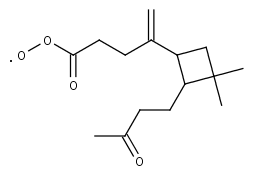
\includegraphics[width=\textwidth]{C141CO3.png}
        \caption{2D `classic'}
    \end{subfigure}
    \begin{subfigure}[b]{0.34\textwidth}
        \centering
        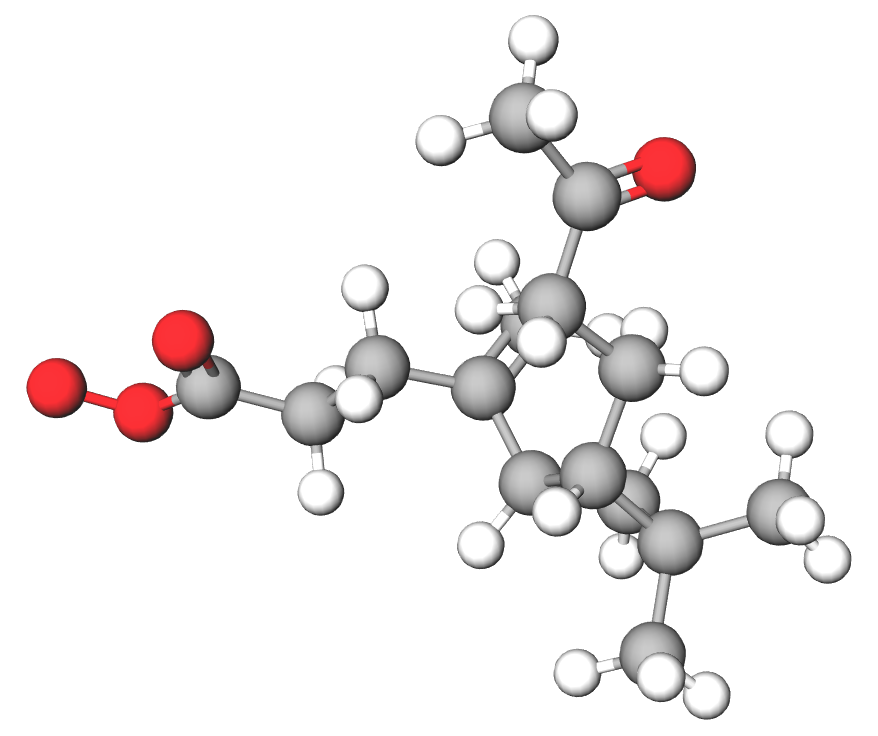
\includegraphics[width=\textwidth]{C141CO33d.png}
        \caption{3D}
    \end{subfigure}
       \caption{\textbf{The molecule \ce{C141CO3} shown in both 2D and 3D node-link structures.} This is a the result of a series of inorganic species reactions and a desocciation from BCARY - the only sesqueterpine in the MCM.  3D visualisation by \citep{mol3d}. }
       \label{fig:mol}
\end{figure}



\afterpage{%
  \clearpage% To flush out all floats, might not be what you want
\begin{landscape}
\begin{figure}[h]
    \centering
    
    \vspace*{-0.02\paperheight}
        \includegraphics[height=1.01\textwidth]{roche.pdf}
    \vspace*{-0.015\paperheight}
       \caption{\textbf{The Roche Metabolic Pathways of the human body. }This example demonstrates the ability to manually represent the complex chemistry of the body using a graph structure. (Original A0 version is available at the source). Source: \citep{metabolic} }
       \label{fig:metabolic}
\end{figure}
\end{landscape}
}

\subsubsection{Using Sociograms To Describe Reactions}\label{sec:mcmgraph}

A collection of reactions representing the chemistry of a region is called a mechanism. The Master Chemical Mechanism \citep{mcm} provides a collection of equations describing the gas-phase chemistry which exists within the troposphere (\autoref{sec:dataset}). In its use in policy, and the evaluation of Air Quality Models (\citep{defra1}), it is often useful to understand the degradation process different VOCs undergo. In general, this may be done using a series of interconnected reactions in the form of a reaction cycle (\autoref{fig:butane}). This type of sociograph shows the directional nature of chemical reactions and the relationships between different species. This has many similarities to a conventional directed graph, except that species (nodes) are sometimes duplicated (for example \ce{OH, HO2, O2} in \autoref{fig:butane}) to aid in the clarity of the figure.

\begin{figure}[h]
    \centering
        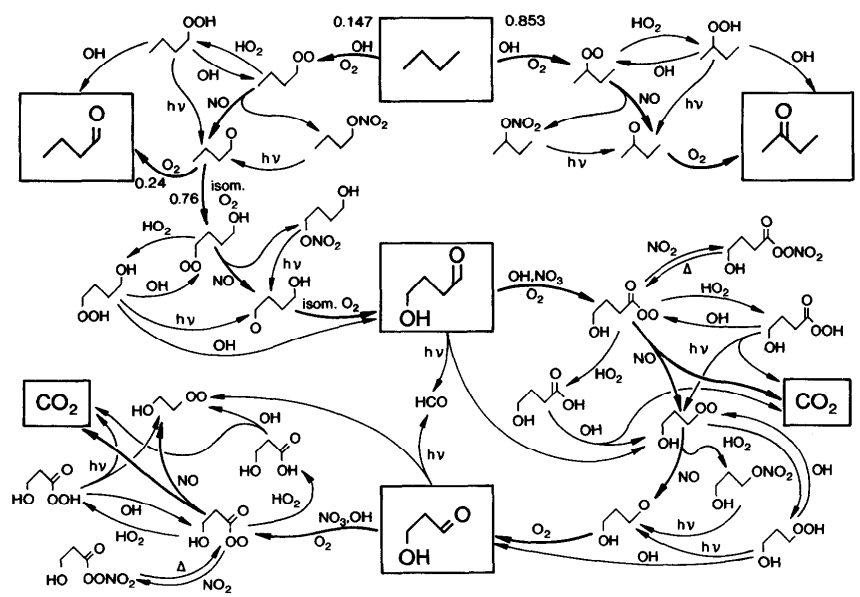
\includegraphics[width=\textwidth]{figures_c1/butane.png}

       \caption{\textbf{A systematic representation of the degregation of butane.} Using this we are able to see the process \ce{C4H10} undergoes before its ultimate demise as carbon monoxide and water. Source: \citep{butane} }
       \label{fig:butane}
\end{figure}


This is an excellent example of how the flow-like nature of a sociogram aids in the understanding of a potentially complex chemical system of 171 organic species and 600 reactions. Evolutionary traits, including the genetic predisposition to interpret shapes faster than text (\citep{sapiens}) make the graph structure a much better method for representing such a system.





\subsection{Modeling Chemistry As A Directed Graph.}

Historically it is shown that the graph format has proven to be an efficient means of understanding the reactions within a mechanism. Traditionally these are constructed manually, with the designer making a series of choices on how best to place, and simplify the chemistry based on their application. As our understanding of chemistry improves and we have started to progress into automated and semi-automated mechanism construction. This makes the construction of mechanisms with tens of millions of species and billions of reaction possible (\citep{protocol}) and is the point where the manual design/simplification of reaction networks becomes infeasible. 

Today automatic graph layouts allow us to generate multivariate and complex graphs quickly \citep{ch3} -This means that, much like in the construction of a mechanism, we can rely on computer-aided design to generate a directed graph representation of the chemistry. \cite{sciamerican} states that "The beauty of a good information graphic is that it can tell a whole story in a single unit of visual content". This is particularly true for the use of directed graphs in chemistry where we can compare different mechanism subsets,(\autoref{fig:meccomp}) or model simulations (\autoref{sec:diurnal}).

However, several problems emerge from the complete automation of a task. Firstly real-world data very rarely reacts how it is expected to. Here networks of high edge density often obfuscate the graph data and produce what is only described as a `birds nest', `hairball' or `ball of yarn' within the literature \citep{ch7}. Although such problems can be shown as moments of turbulence, they encourage a greater understanding of the graphic design process and can catalyze to merge unique ideas into an effective visualisation \citep{goodideas} - much like the composite metaphors in \autoref{ch1}.


Having established that a graph network ties in both modern and historical methods for representing relational data, we now look at how to present the graph, both in syntax (\autoref{syntatic}) and semantics (\autoref{semantic}). 



\section{Graph Syntatics}\label{syntatic}

 Syntactic representation considers how best to distribute information on a page for maximum impact. This can be seen between the force-directed graph (top) and geographical location (bottom) layouts in \autoref{fig:worldmap}. Although the geographical layout gives a more accurate representation of the distances between unconnected nodes (airports), a force-directed graph provides greater insight into the relationships (flights) between each airport. This highlights the importance of choosing a suitable syntactic representation to highlight the features of interest. The remainder of this section discusses the syntactic choices required for the visualisation of a complex chemical mechanism. 

 
\begin{figure}[H]
     \centering 
      \begin{subfigure}[b,black]{.9\textwidth}
         \centering 
     \includegraphics[width=\textwidth]{figures_c1/layout/layoutforce.png}
     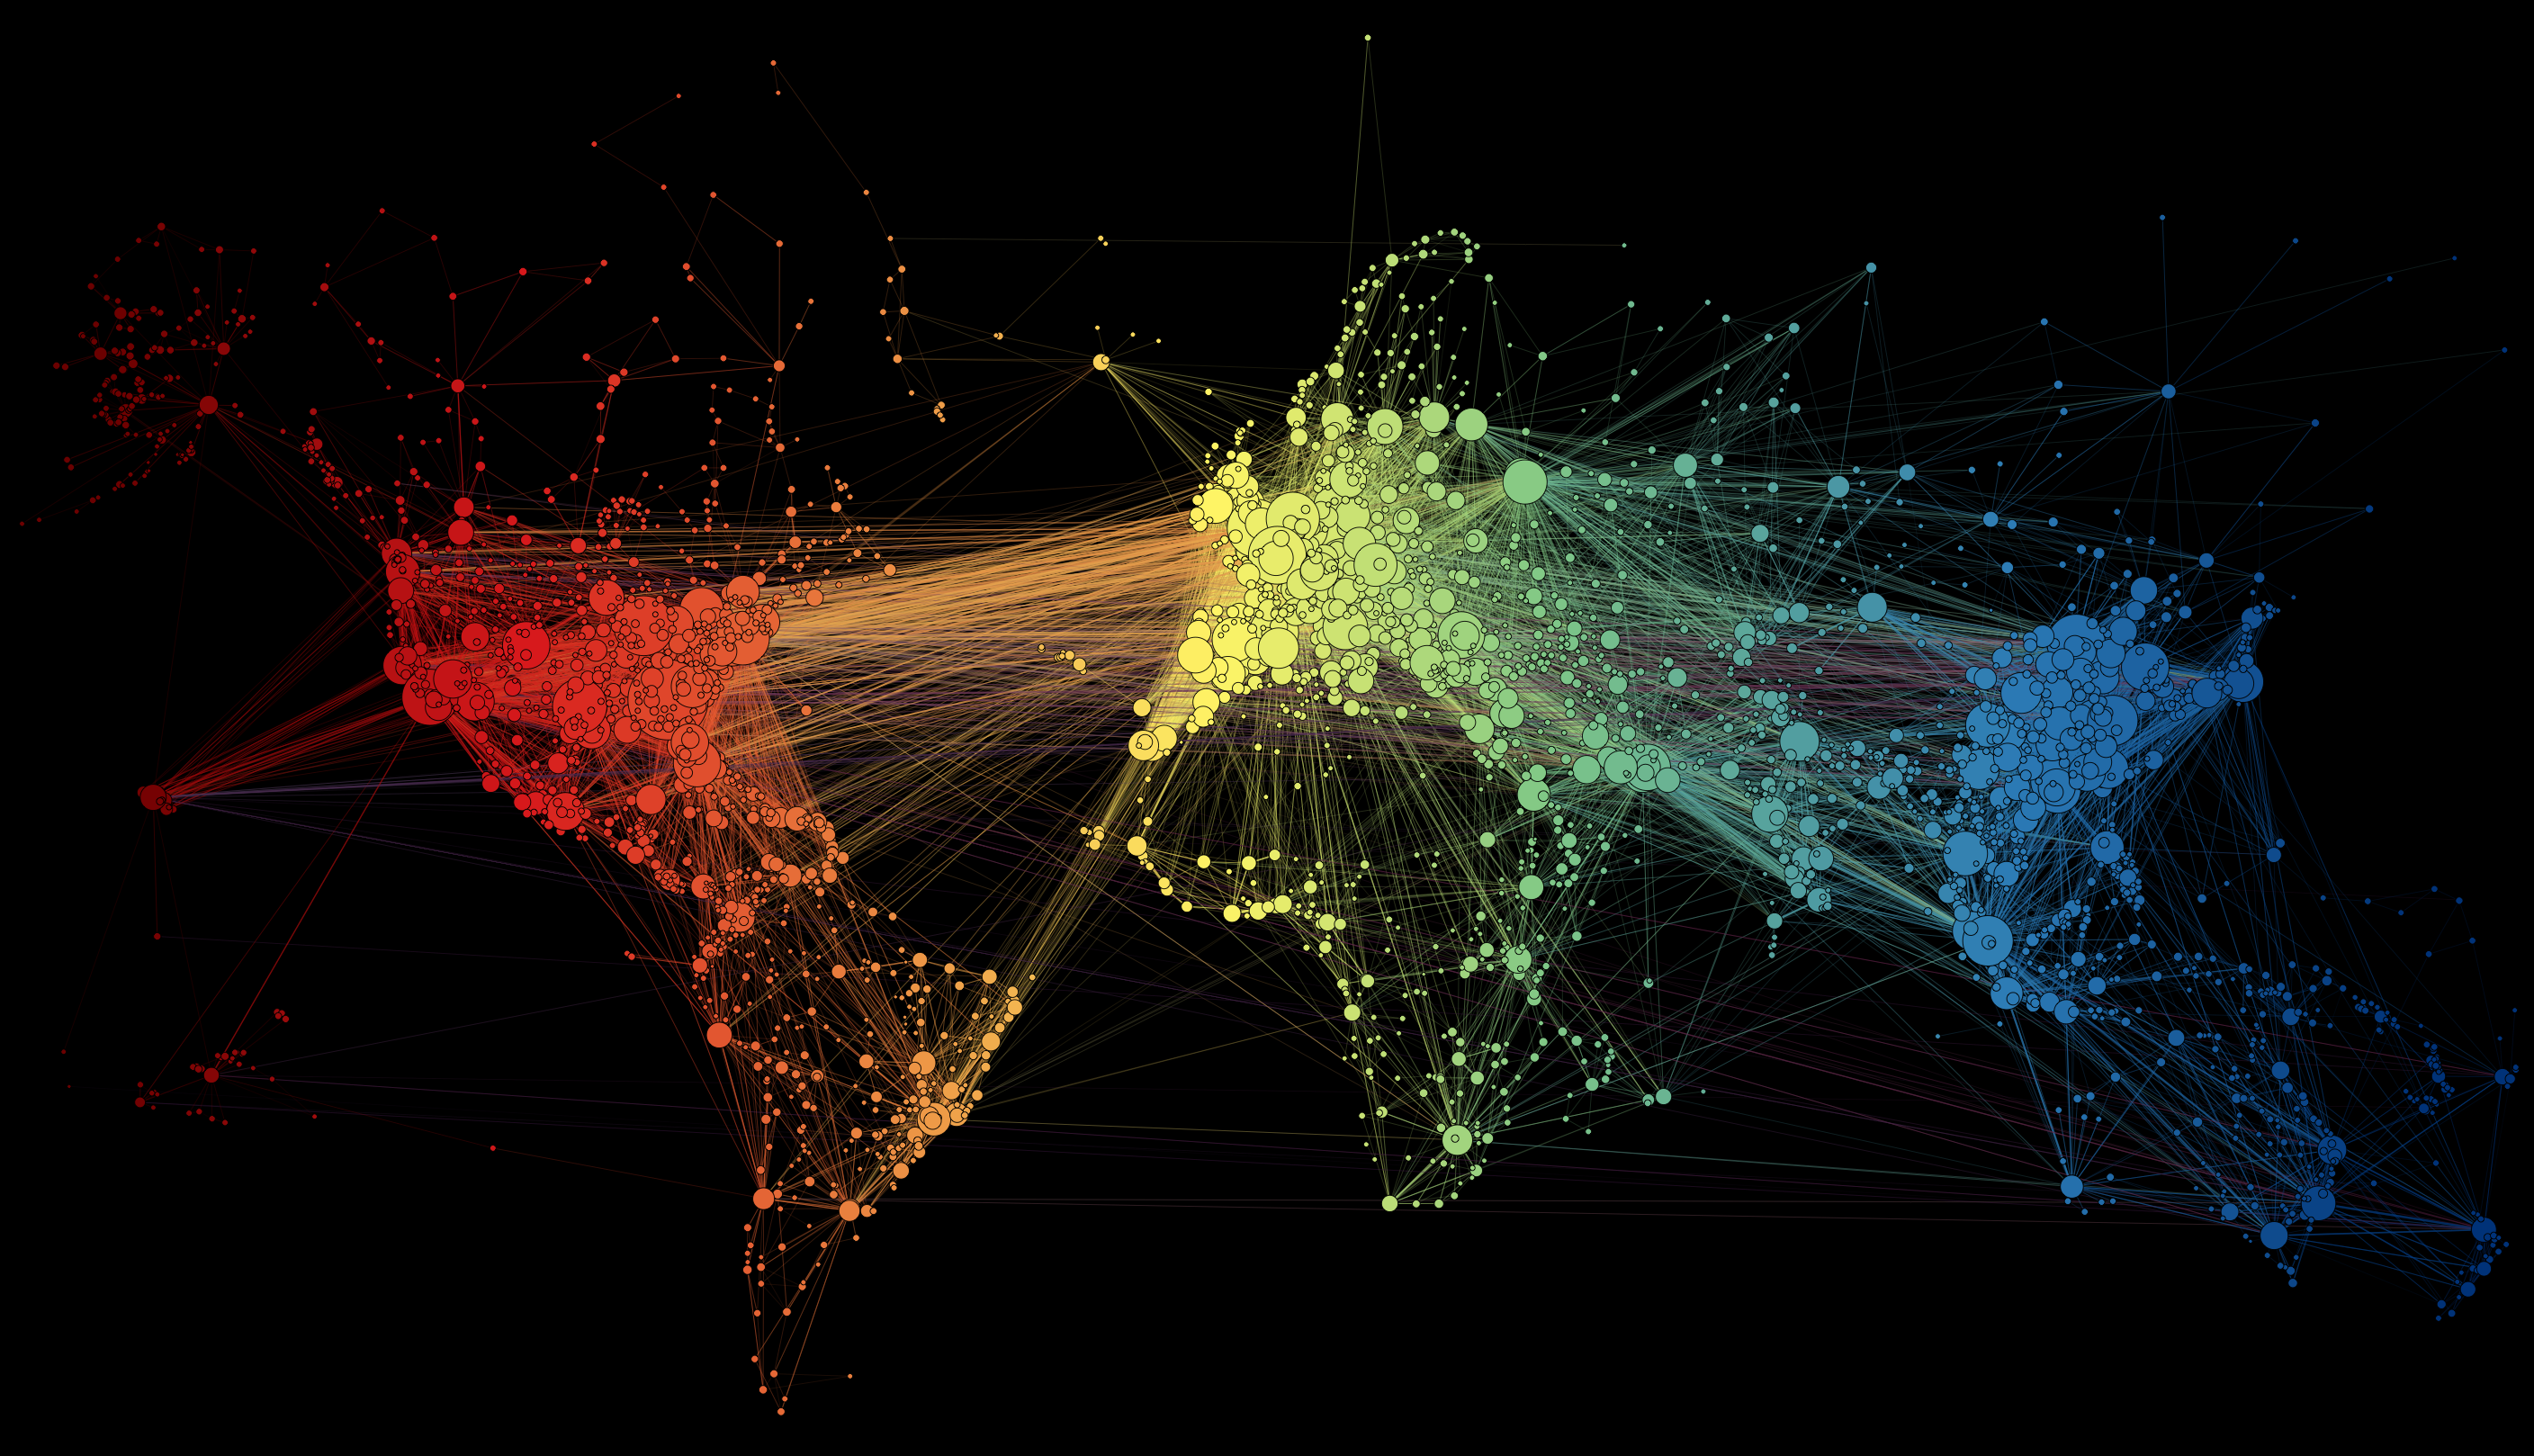
\includegraphics[width=\textwidth]{figures_c1/layout/layoutgeo.png}
     \end{subfigure}
        \caption{\textbf{Comparison of different representations of flight data by \citep{worldmap}.} The top figure shows the data represented by a force-directed graph layout (described below) and a Geo-layout showing each point at its location on the Earth.}
        \label{fig:worldmap}
\end{figure}


\subsection{Selecting The Correct Evaluation Criteria.}
As chemical networks provide a wealth of information on the reactions within a system, this can prove challenging to user cognition and computational resources \citep{ch1}. In selecting the best possible graph layout, there are many metrics designed around the improving of visualisations aesthetics \citep{metricgraphaesthetics} however, these have often only been evaluated with a handful of criterions in mind. Such metrics can make it difficult to accurately quantify the changes in user-readability, especially if they are not treated as originally intended \citep{eyetrack}. 


\subsubsection{Edge Crossing} \label{sec:edgecross}
One of the greatest limitations to understanding a graph is the number of overlaping (crossing) edges \citep{humanaesthetic}, especially since users often spend most of their time looking at the edges of a graph in order to understand it \citep{eyetrack}. 

There exist several type of graph layout algorims which aim to reduce the amount of overlapping edges in a graph. The two most common ones are force-directed and orthogonal. Orthogonal designs are those of straight edges at 90 degree angles, such as in architectural or circuit schematics (\autoref{fig:orthogonal}). Force directed graphs (\autoref{sec:forcedirected}) are a graph layout is designed to simulate a phsical system, where node positions are the result of the push and pull of the edges between them. In the task selecting nodes from a specific path, users were twice as more accurate using this layout than the orthogonal one \citep{eyetrack}.


\begin{figure}[H]
    \centering
        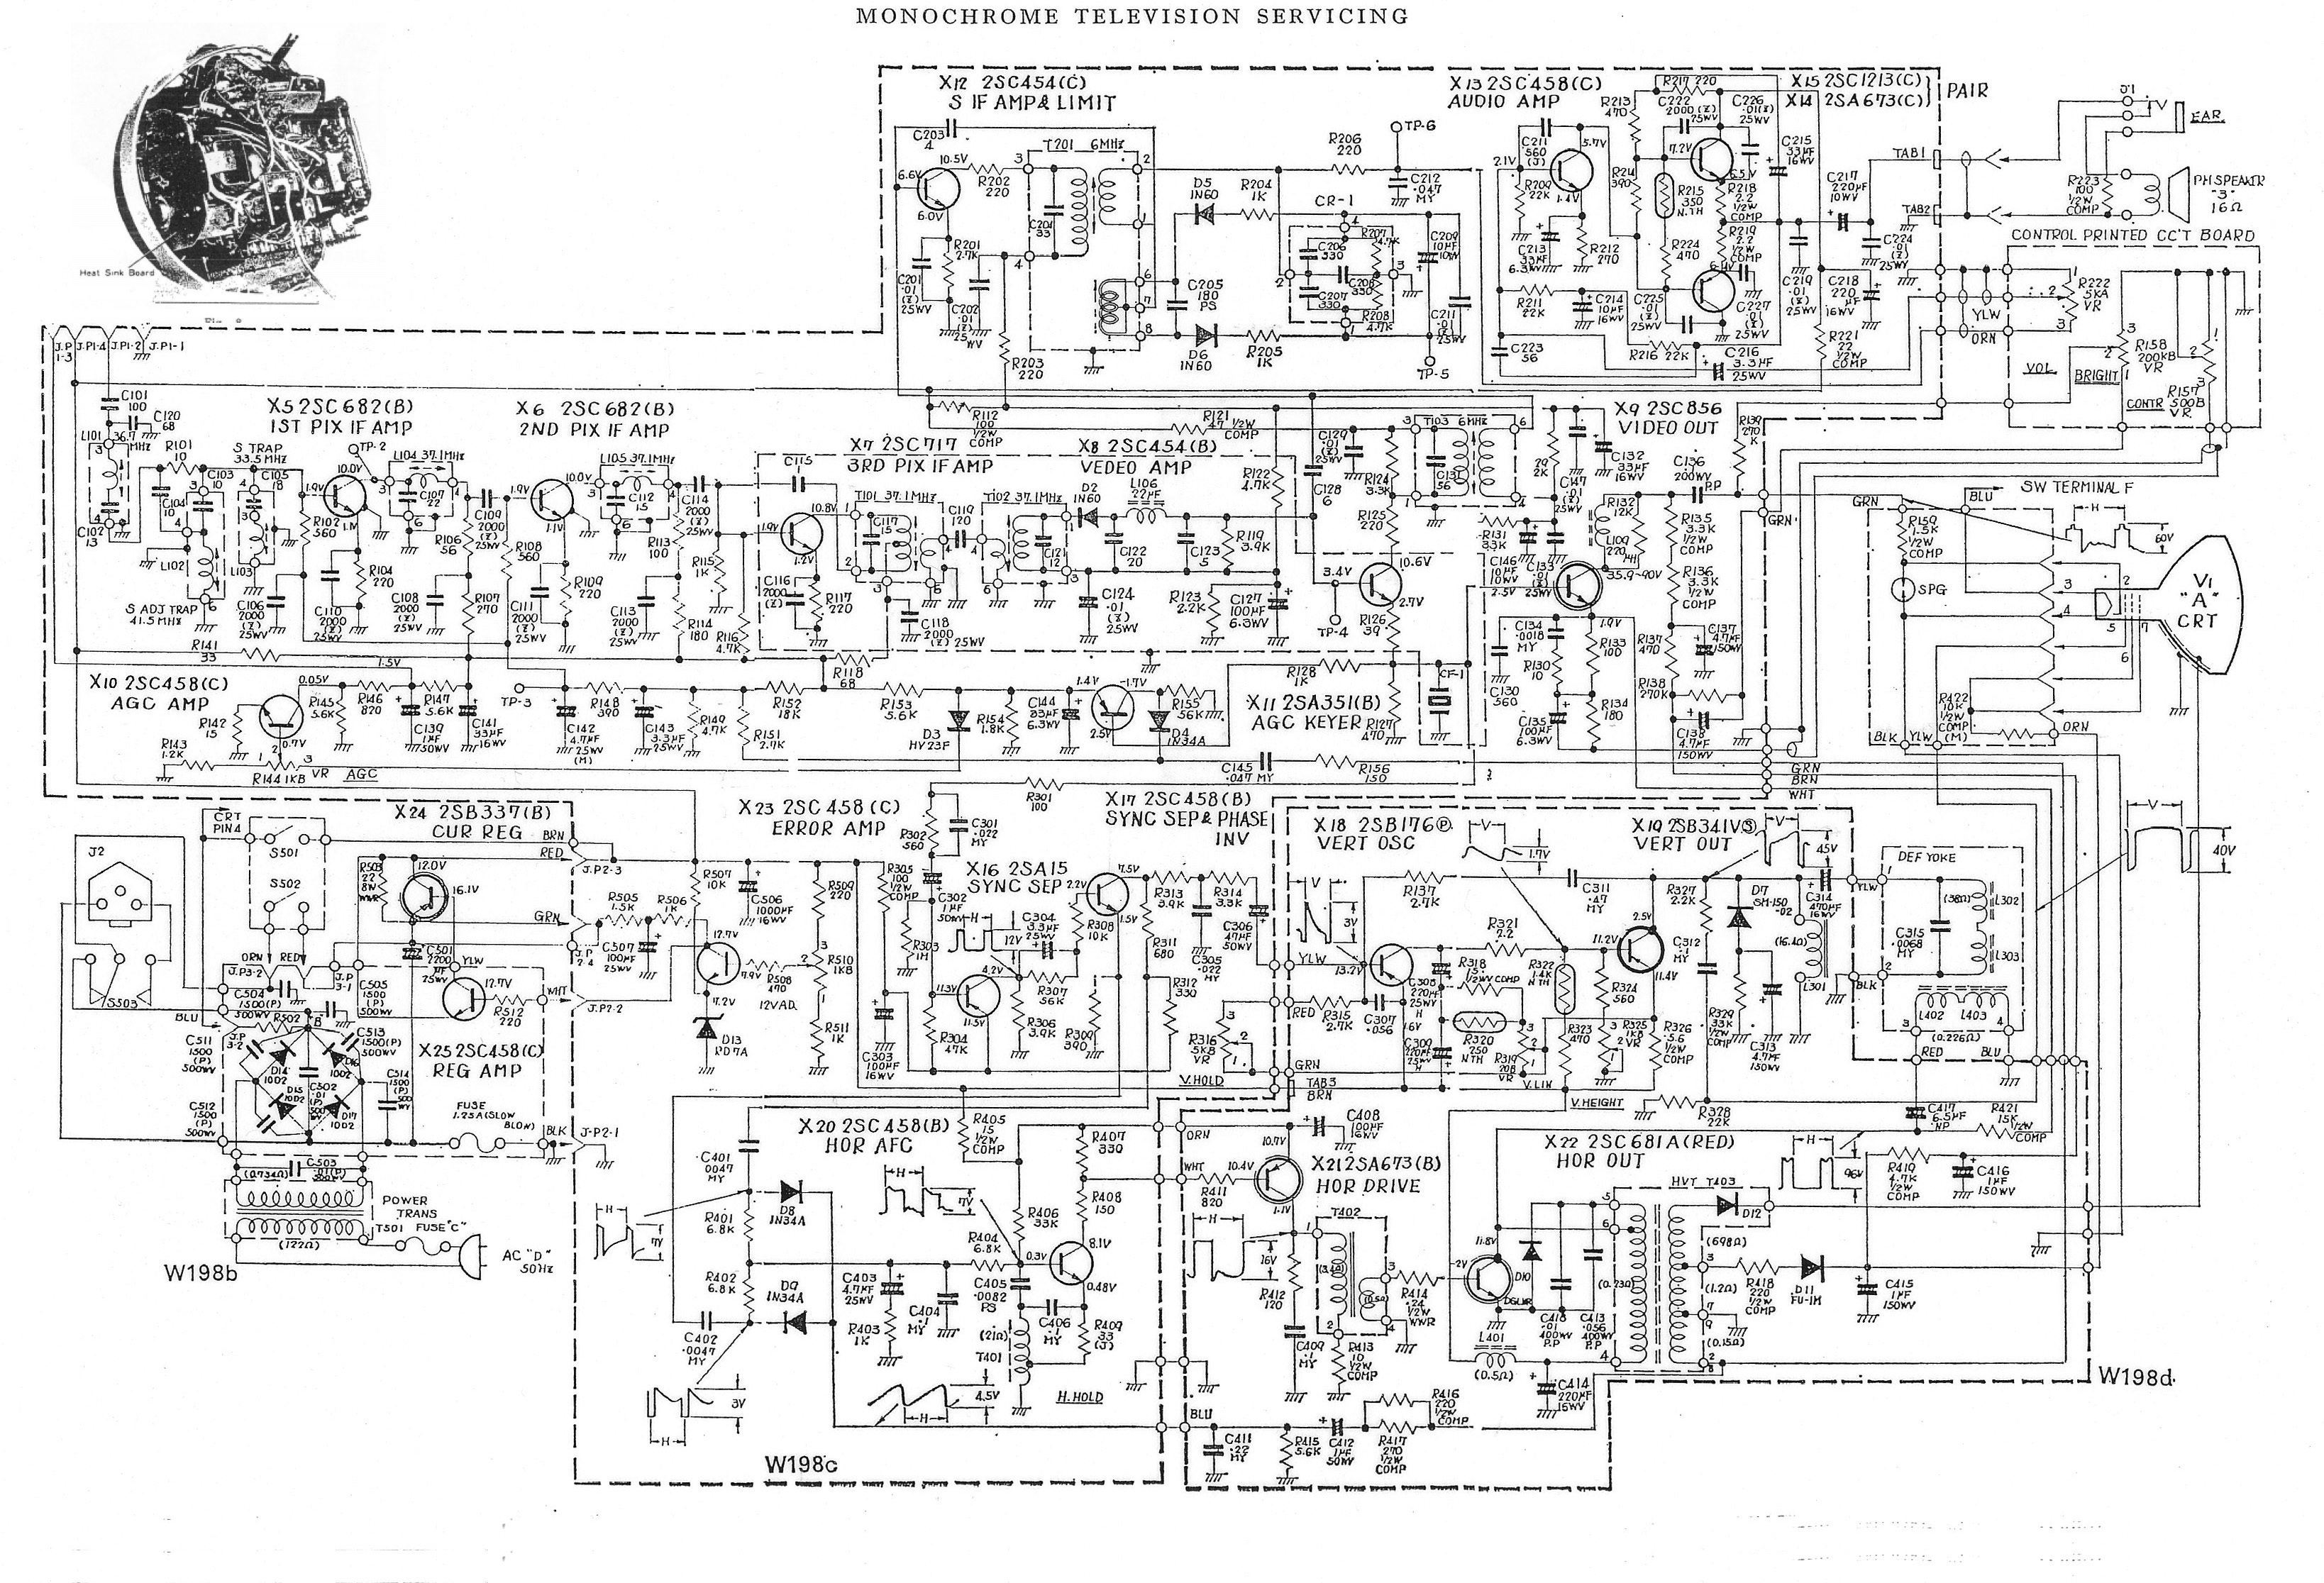
\includegraphics[width=\textwidth]{tvschematic.jpg}
       \caption{\textbf{An orthogonal circuit schematic of the Model 3 240 portable cathode ray tube television.} The circuit schematic of the television (top left) shows a much simpler representation of how different components within the television are connected.  Source: \citep{orthogonaltv} }
       \label{fig:orthogonal}
\end{figure}



 % 
 % Finally, the use of bends may be misleading as users can perceive them as multiple separate objects \citep{aestheticsgraphvis}.
    
 
\subsubsection{Node Distribution And Overlap}\label{sec:ndist}

The distribution of nodes across the page can both hinder or increase the readability of a graph - especially since larger nodes may obscure smaller ones at the same location. \cite{ch6graphredability} found that graphs with an equal node distribution across space, at a medium edge length greatly impoved graph readbility - with node distribution and graph-symmetry ranking second in a study on user preference on graphs. 

In addition to selecting the best graph layout, there exist several methods in which overlapping nodes may be removed - an issue that is sometime diffucult by the treating of nodes as `point masses' within an algorithm \citep{nodeoverlap}. \cite{IPSEPCOLA} explains that there are usually two methods for reducing the number of overlapping nodes in a graph, these are:


\begin{itemize}
\item [1.] Create a layout design capable of taking node size (e.g. \citep{nons}) into consideration. These designs tend to be layout specific and not absolute in removing all overlap between nodes. 
\item [2.] This requires a level of post-processing in the form of a `layout adjustment'. Here we reposition nodes after a chosen layout has finished computing. The drawback of this method is that information contained in the graph's shape may be degraded. This can be done through the use of collision detection, or moving nodes to the centre of the vernouli cells \citep{novern}. 
\end{itemize}




\subsection{Automated Graph Drawing Layouts}\label{sec:drawing}


In their design and evaluation, automatic graph drawing algorithms are created to minimise a specific criterion. This subsection will compare a number of graph layouts and make a verdict on which one is most suited for the representation of troposheric chemistry. This task shall use the mechanism extracted in \autoref{tab:icsmetric} to represent the VOC's within the Beijing city - a real world case study using the MCM. 

To do this we begin by exploring hand-drawn / map inspired graph layouts (\autoref{sec:handdrawn},\autoref{sec:merc}), eventualy ending at a number of  automated force-directed graphs (\autoref{sec:forcedirected}).


\subsubsection{Replication Of Hand-Drawin Methods}\label{sec:handdrawn}
With the rise of computation, many traditional visualisations adapted for the computer-aided generation. Fields of architecture and circuit design adopted computational software to alleviate some of the difficulties presented by large or complex designs. Similar ideas such as the use of automatically generated transit maps can be used to link chronological or topological items such as ideas \citep{memory}. \autoref{fig:mem} shows all the possible paths for the oxidation of methane to produce carbon dioxide (and water), using the MemoryMap algorithm \cite{memory}. Although such methods can be useful in showing isolated pathways, they provide a convoluted representation of large interconnected systems and require some manual intervention. 


\begin{figure}[H]
     \centering
     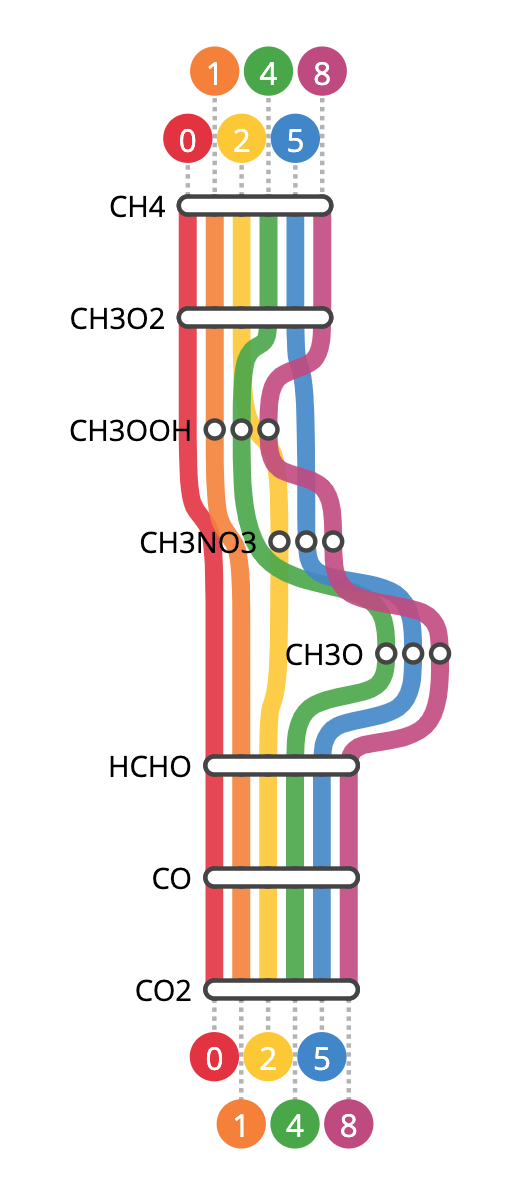
\includegraphics[width=0.25\textwidth, angle=0]{figures_c1/layout/memory.png}
         \caption{\textbf{A transit map showing all the possible routes from methane to carbon dioxide.} This was drawn using MemoryMap \citep{memory} and uses a version of the MCM methane subset, where carbon dioxide has been introduced.}
        \label{fig:mem}
\end{figure}





\subsubsection{Projection Based}\label{sec:merc}
One of the oldest fields of data visualisation fall in the realm of cartography. Here the shapes and distances between points on the surface of the earth (an oblate spheroid) are mathematically mapped onto a 1D plane for graphing purposes \citep{projections}. Since the process of dimensionality reduction will produce inherent distortions within the final product, we end up with a range of map projections, with each striving to achieve a different aim (\autoref{fig:projections}). The Pierce Quincuncial, for example, is a conformal mapping technique mapping the surface of a sphere to a square with minimal deviation in scale and the ability to be tessellated in all directions. The Mercator, on the other hand, is a cylindrical projection which grew in popularity due to its unique ability to represent any course of constant bearing\footnote{Also known as a `rhumb', or `loxodrome', and consists of an arc crossing all meridians of longitude at the same angle.} as a linear segment within the shipping and navigation industry.  Finally the waterman butterfly presents the globe as a truncated octahedron. This allows for the reconstruction of a 3 dimensional world from a 2D plane (ie a printed sheet). 

\begin{figure}[H]
     \centering
      \begin{subfigure}[b]{.25\textwidth}
         \centering
     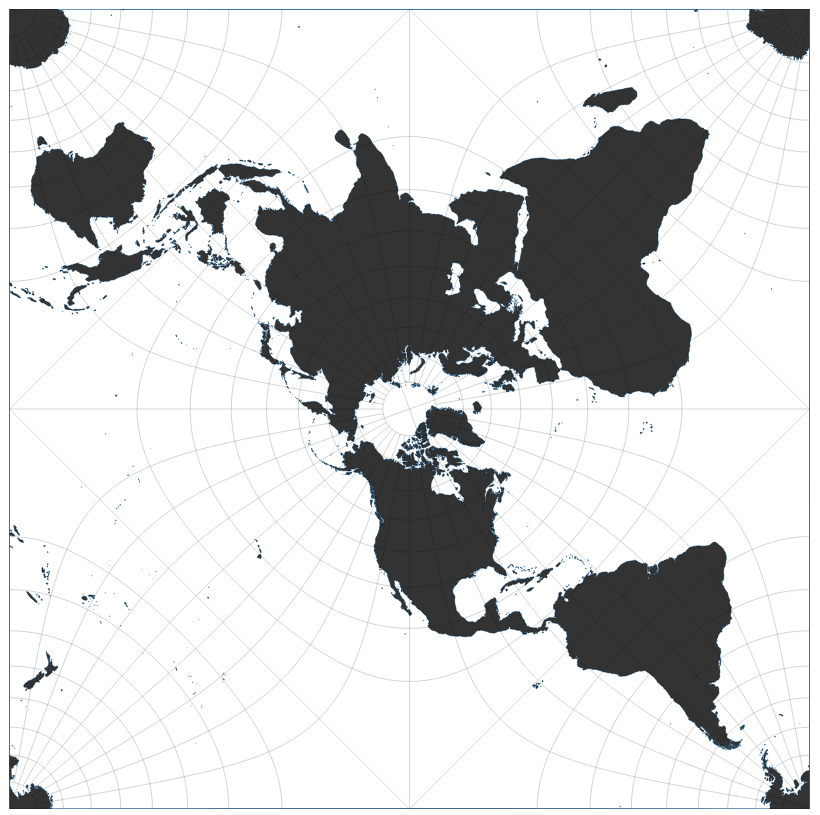
\includegraphics[width=\textwidth]{figures_c1/layout/pierce.png} \caption{Pierce Quincucial}
     \end{subfigure}
    \begin{subfigure}[b]{.3\textwidth}
         \centering
     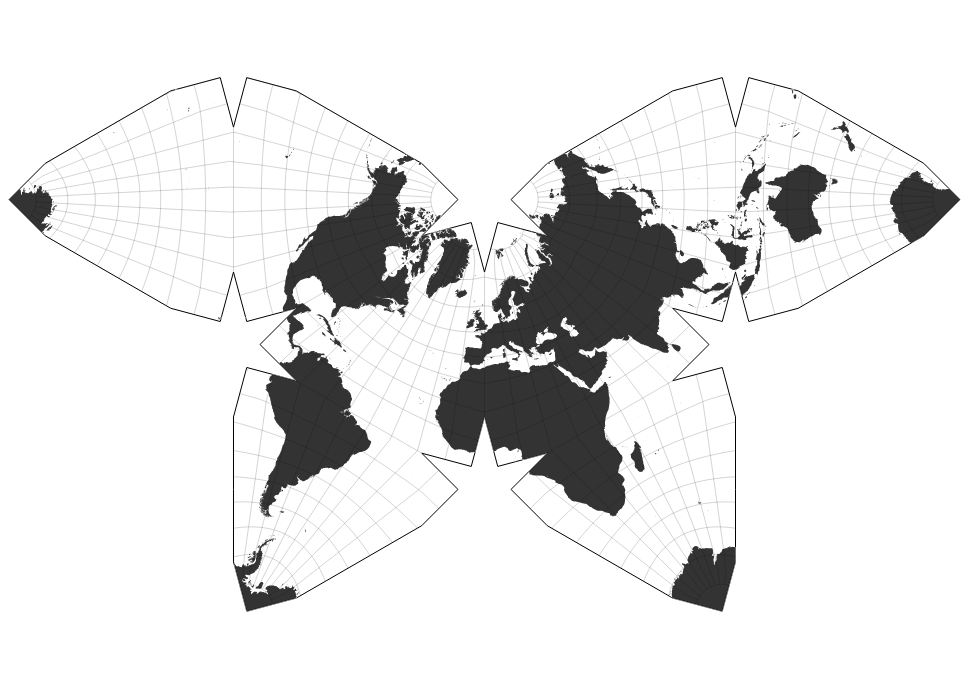
\includegraphics[width=\textwidth]{figures_c1/layout/waterman_butterfly.png}
     \caption{Waterman Butterfly}
     \end{subfigure}
     \begin{subfigure}[b]{.3\textwidth}
         \centering
     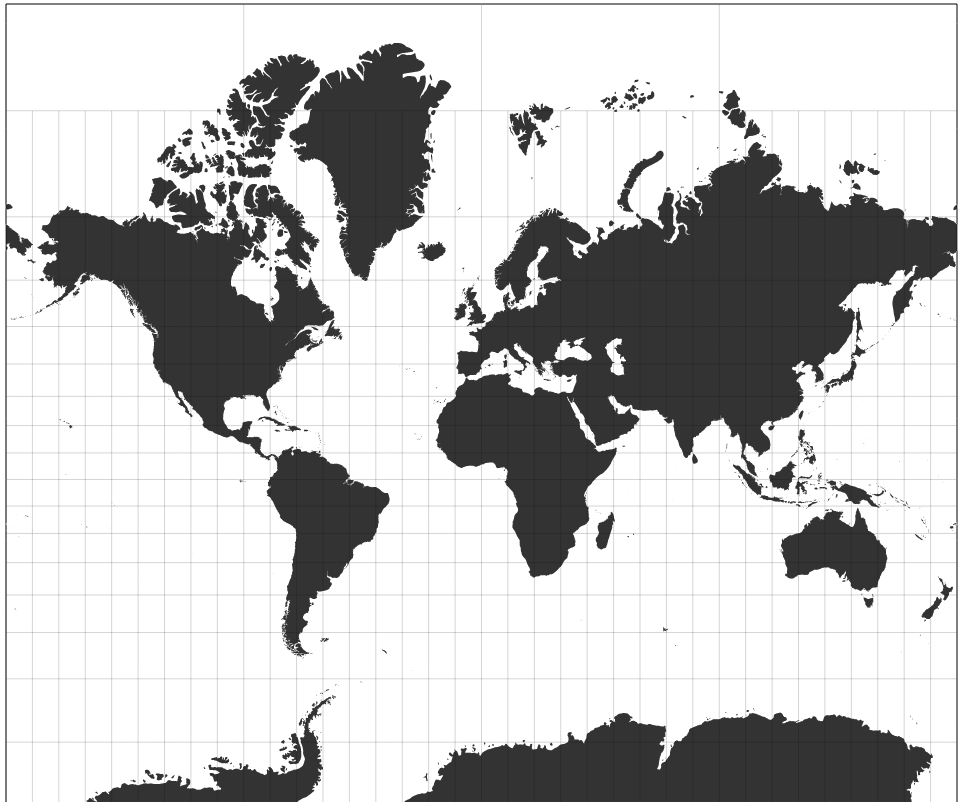
\includegraphics[width=\textwidth]{figures_c1/layout/mercator.png}
     \caption{Mercator}
     \end{subfigure}
        \caption{\textbf{A selection of map projections.} These have been created using DataDrivenDocuments \citep{d3} and show a range of methods for mapping the spheroid shape of the Earth onto a 2D plane. }
      \label{fig:projections}
\end{figure}



\begin{figure}[H]
     \centering
      \begin{subfigure}[b]{.495\textwidth}
         \centering
     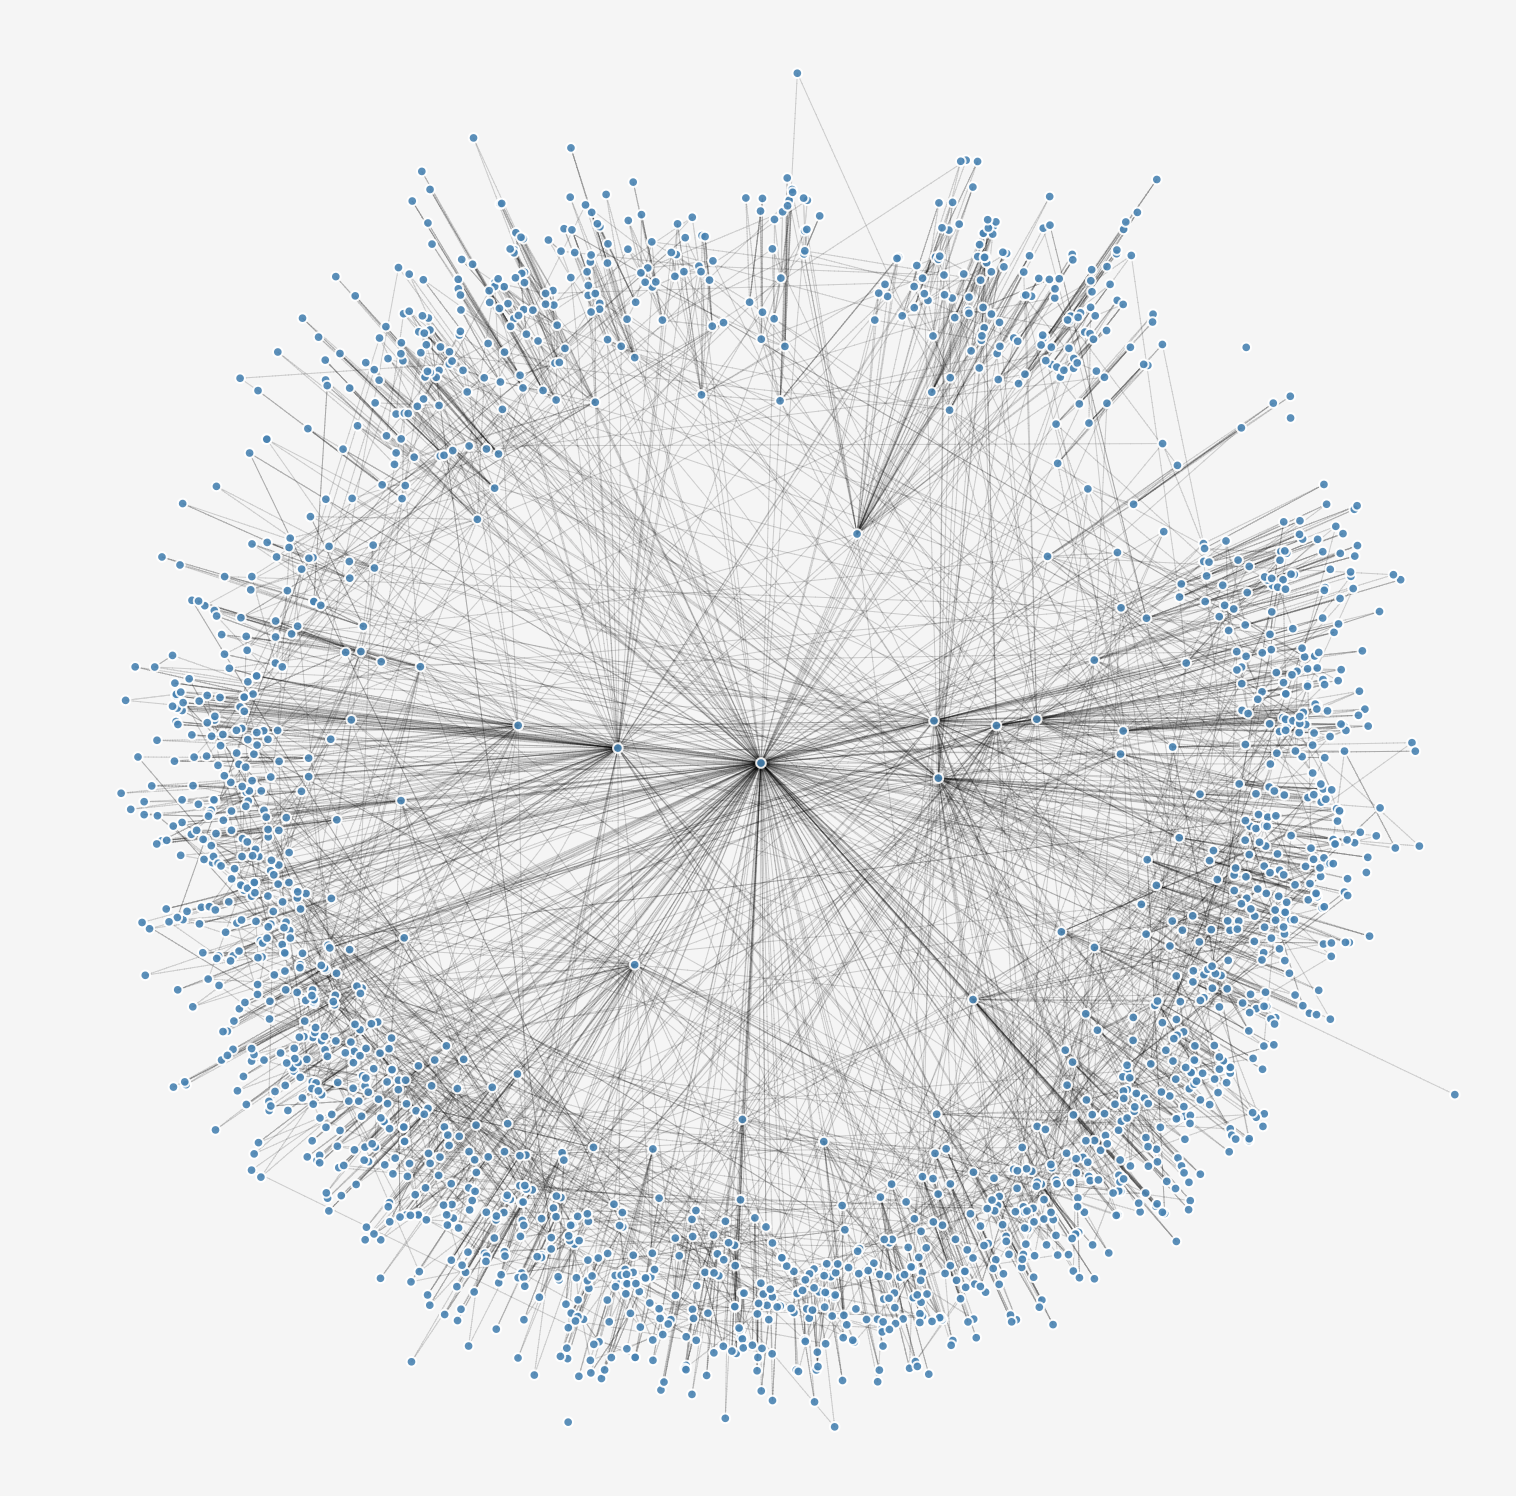
\includegraphics[width=\textwidth,angle=90]{figures_c1/layout/merc1.png}
         \caption{The Mercator graph.}
     \end{subfigure}
    \begin{subfigure}[b]{.495\textwidth}
         \centering
     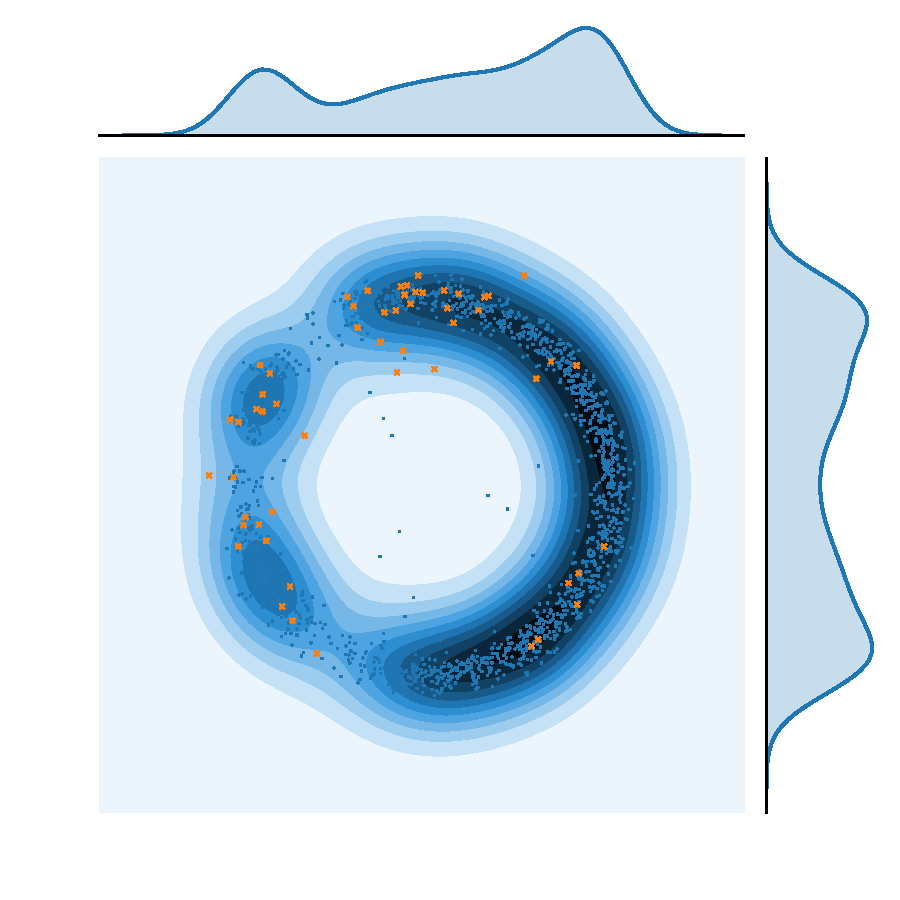
\includegraphics[width=\textwidth]{figures_c1/layout/merc_aphh.pdf}
     \caption{Mercator species distribution}
     \end{subfigure}
        \caption{\textbf{The Mercator Projection.} (a) represents output from the mercator graph layout algorithm. (b) provides a kernel density analysis of the node distribution within this. Here (a) shows graph structure by revealing the density of connections between different nodes, whilst (b) reveals the density of nodes at a specific location. }
        \label{fig:merc}
\end{figure}

More recently, the mathematics of mapping a large dimension onto a simpler one has been applied to the problem of graph representation. \citep{mercgraph} uses the latent hyperbolic geometry of the Mercator layout to provide a 2D embedding for complex real-world networks. This produces a polar representation ($r$ and $\theta$) of the system, where relationships of related species are of the same angle ($\theta$), with nodes of a high degree are closer to the centre (low $r$ value, where $r$ is the radius from the centre). Using the chemical mechanism from the APHH  Beijing campaing (described above), this produces a layout, (\autoref{fig:merc}) where (a) shows the graph-based representation including links, and (b) shows the density distribution for all nodes. \autoref{fig:merc}b shows that primary emitted species (orange dots) are uniformly (radially) distributed for angles and \autoref{fig:merc}a reveals that influential nodes with a high degree (highly connected) are located close to the centreof the graph. Although the Mercator embedding does reduce the `hairball' problem experienced by other layouts, it does not take edge weight/direction or self-loops. This means that it works well for the representation of the general network layout, but cannot be used for advanced data exploration concerning simulation results.  



\subsubsection{Force-Directed}\label{sec:forcedirected}

Force-directed graph layouts are the results of the Spring-Electrical model. This was first introduced by \citep{Eades} and further improved by \citep{raingold}. Force-directed layouts are in essence a simple physics simulation of like-charged particles represnting the nodes. These particles act similarly to protons which experience Coulomb repulsion and try to get away from each other. If there is a relationship between two nodes, a spring-like attractive force is introduced, drawing the nodes back together. 

In the case of a weighted graph, where each link (or relationship) has a value associated with it, we can adjust the spring coefficient of the attractive force to reflect this. This results in a layout where strongly connected objects are drawn together, and weakly connected ones further away. Uses for this type of representation have been shown biology, social networks, and with this thesis atmospheric chemistry \citep{ch3,ch4}.

Next we describe the Barnes-Hut algorithm, a mapping algorithm which builds a hierarchical tree of the data by splitting a plane into quartiles. This is used within the many force-directed graph layouts, including those of Force Atlas 2 and Yifan Hu, described shortly. Once this has been done a selection of four different layout algorithms shall be discussed.  


\paragraph*{Barnes Hut Algorithm}
Since calculating the attractive/repulsive forces for each node of a large graph can be computationally intensive, many force-directed layouts rely on the Barnes-Hut approximation. This solves the N-body problem of pairwise reactions between nodes, $O(n^2)$, by approximating long-range reactions by grouping such nodes and applying a single action on their centre of mass- reducing the computational time to $n \log n$.  

To do this, first, a spatial index of each node is constructed (see below). This can either be done using a quadtree (2D) or octree (3D).Followign this we calculate the centre(s) of mass, allowing us to aproximate the repulsive forces of a force-directed graph.

\textbf{Quadtree Construction:}
A quadtree is the recursive partitioning of two-dimensional space into a set of quadrants (a set of 4 squares). This process is repeated, with each square then being divided into four itself, until there is only a single point within a cell. This converts a network, into a hierarchical tree representation of the nested quadrants in which each point resides (a quadtree), \autoref{fig:quadgroup}. 


\begin{figure}[H]
 \centering
    \begin{subfigure}[b]{.3\textwidth}
  \centering 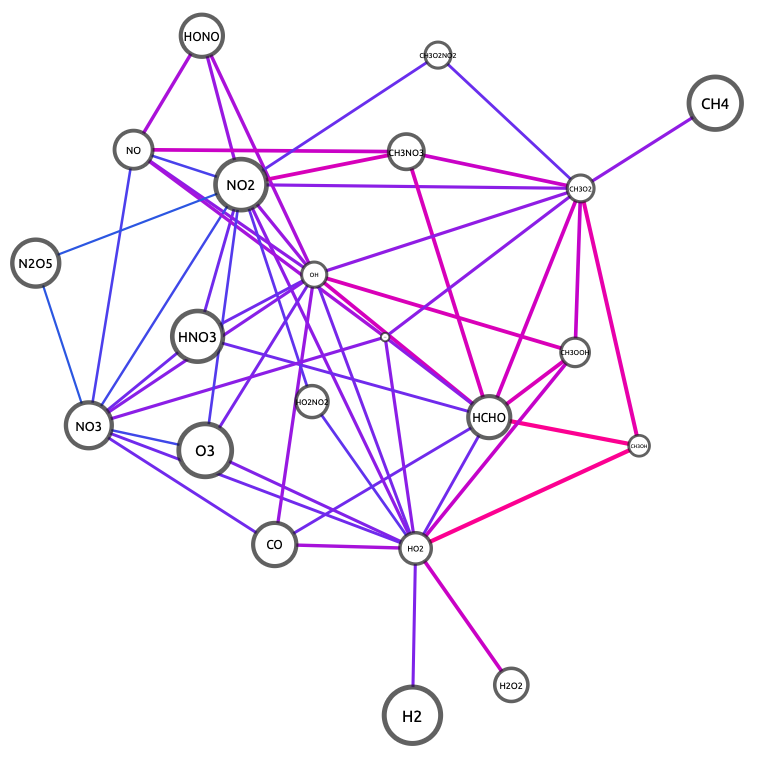
\includegraphics[width=\textwidth]{figures_c1/layout/methanequad.png}   
  \caption{Methane Graph} 
  \label{fig:quadmeth}
 \end{subfigure}
 \begin{subfigure}[b]{.6\textwidth}
  \centering 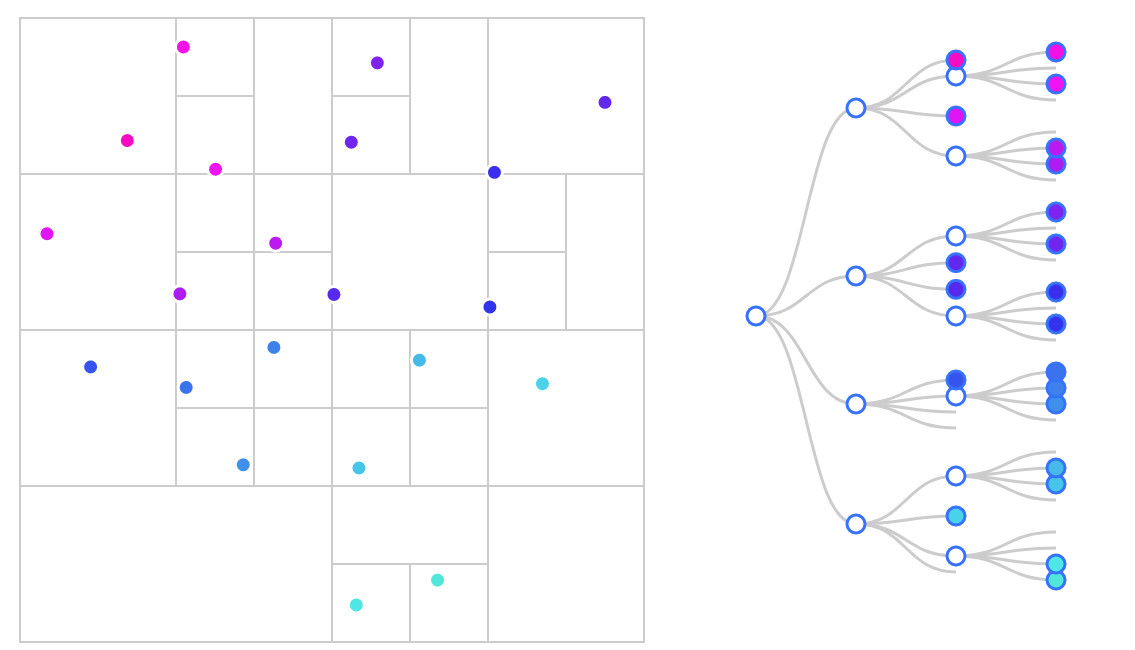
\includegraphics[width=\textwidth]{figures_c1/layout/quad.png}
 \caption{Quadtree constructed from \autoref{fig:quadmeth}}
\label{fig:quadtree}
\end{subfigure}
\caption{ \textbf{Demonstration of the formation for a quadtree from a force directed graph of Methane (including inorganics)}. (a) shows the force directed graph of Methane from which the quadtree has been constructed- edge colours represent the flux between species. Here we partition the area into 4 and start at the top-leftmost cell. This is then partitioned into 4 itself in a recursive process until there is only one point per cell. We repeat the process to any remaining cells in a clockwise manner (b). The hierarchical tree (b right) shows the containing structure for each node. Here the colours represent the order in which nodes have selected (starting at pink and ending in blue). }
\label{fig:quadgroup}
\end{figure}

Having defined this we move on to looking at the graph layouts.

\paragraph{Force Atlas 2}
The force atlas two \citep{fa} algorithm is a force-directed layout designed primarily for scale-free\footnote{A network whose degree distribution follows a power law (7 degrees of separation). This is described in \autoref{ch3}.} network spatialization. It is primarily designed for the use of networks consisting of 10 to 10,000 nodes and uses barns-hut approximation for the calculation of forces. Attractive forces are derived from the spring-electric model ($F_a = -k.d$), where k is the spring constant and d is the distance between the two nodes. Optional features for the graph include dissuasion by degree (separating nodes with a high number of total links/reactions), logarithmic attraction forces, adjustable gravity (attraction the centre of mass of the system to prevent disconnected components from drifting away) and collision detection to prevent overlapping nodes. Finally an adaptive cooling scheme is applied, where the overall energy of a system is gradually decreased, allowing the nodes to settle into a low energy states.

\paragraph{Yifan Hu}
The Yifan Hu graph layout \citep{yh}, is a multi-level graph drawing algorithm which uses the Barnes-hut algorithm with an octree layout. As with the force atlas algorithm, Yifan Hu also has an adaptive cooling aspect to it - meaning that as the algorithm is run its energy is progressively reduced, allowing the system to settle within a low energy state.  

\newpage

\textbf{The main difference within the algorithm, however, is the use of the multilevel approach. This has been applied to graph partitioning [11,12,23], matric ordering [24] and the travelling salesman problem [5]. This works by graph coarsening (coalescing neighbouring nodes and weighting them), running the algorithm on the course graph, prolongation and then refining the results. This produces an algorithm that runs faster than the Force Atlas, however, is constrained to only working on un-directed edges.
}

\paragraph{OpenOrd}
A force-directed graph algorithm capable of scaling to very large graphs \citep{openord}. OpenOrd uses simulated annealing (see below), which has 5 distinct phases. These are each run for a fraction of the total number of iterations and mimic the different states experienced when heating/cooling a physical object (liquid, expansion, cool-down, crunch and simmer) - hear each state describes the amount of energy asigned to the nodes within the force simulation. In additon to this the OpenOrd algorithm applies a degree of edge-cutting to remove a percentage of edges experiencing the most stress within the physical system. This allows the network to open out into a more aesthetically pleasing layout. 


\paragraph*{Simulated Annealing}
Most iterative layouts are updated interactively from some initial configuration in attempt to reach the lowest energy state of the system. In most cases this results in a minimum configuration; however this is generally a local minimum rather than the desired global minimum (the optimum low energy state of the entire system) \citep{nicelyanneal}. To overcome this, the work of \cite{metropolis}, which was later formulated in general terms by \citep{kirkpatrick} was used to lay the foundation for simulated annealing algorithms.

Annealing is usually used to describe the slow cooling applied to liquids for them to reach a crystalline (totally ordered, minimum energy) form. Relating this to the spring-electrical model, it can be shown that if the atoms(nodes) are cooled too rapidly (losing energy quickly and coming to a quick stop), they will form amorphous structures representing the local minima, as opposed to the desired global one.  If cooled slowly, our graph is allowed to find a thermal equilibrium at every temperature. Working from this idea, a slow cooling constant is applied, whilst occasionally supplying the system with short bursts of energy, that may allow it to overcome local minima. 


\paragraph{tsNET}
t-Distributed Stochastic Neighbor Embedding (t-SNE) is a dimensionality reduction techneque which mimics the style of a force-directed graph (this is discussed in \autoref{sec:overcrowd}). tsNET\footnote{A play on t-SNE and network.} is a graph drawing algorithm which levarages the non-linear dimensionality reduction capabilites of the t-SNE algorithm \citep{tsne}. This works by first computing the shortest-parth distances between all nodes to produce a distance matrix. This distance matrix is then used to construct a cost matrix which consists as the sum of three terms:

\begin{enumerate}
    \item A measure of the divergence between picking paris of low- and high-dimensional datapoints.
    \item A compression factor known to reduce the t-SNE optimisation time, taken from \citep{tsnetcompression}.
    \item A repulsion term to prevent nodes clumping together.
\end{enumerate}
    
Node positions are then determined by the mimimisation of the cost matrix using gradient decent - an optimisation algorithm used to minimise a function by iteratively moving in the direction of the steepest descent. 

\textit{Note: Although tsNET makes for a good alternative to classical graph layouts, it does not take link direction into account. }



\section{Selecting The Best Graph Drawing Layout.}

\autoref{sec:edgecross} explained the importance of removing overlapping edges and \autoref{sec:ndist}, the desire of having a well distributed graph layout. This subsubsection builds on those criterions, assessing all the graph layouts described within this section (Mercator, Force Atlas 2, Yifan Hu, OpenOrd and tsNET). These all use the chemical mechanism representing species within the APHH campaign in Beijing \citep{aphh}. Here we look at the distribution (\autoref{sec:nodedist}) and density (\autoref{sec:nodedensitya}) as they affect a users ability to isolate the shortest path (fastest flux).

 Force-directed graphs place a greater emphasis on node positions,





Criteria, such as the ability to isolate the shortest path (in this case the fastest flux), are essential in determining the usefulness of a graph. Comparing different layouts \citep{eyetrack} found 68\% of user-chosen routes to reflect the shortest path between them. 

This is due to the force-directed layout placing a greater emphasis on node positions and distance than other layouts. For comparison, the same study found this to be 40\% for hierarchical layouts and only 2\% for orthogonal ones. In this subsection, I look at the use of different graph layouts, and their effect on the user readability of a graph. 


\subsection{Node Distribution}\label{sec:nodedist}

\autoref{sec:ndist} explained the importance of node distribution within a graph visualisation. Additionally \cite{ch6graphredability} explains that if we partition the viewing medium into quartiles, and poopulate each quadrant with an equal number of nodes (homogeneity), this drastically improved the usability and symmetry of a graph.

The problem is that for complex real-world graphs is that they often contain nodes with many reactions between them (\autoref{fig:fullmcm}). Such regions of dense, indecipherable links (often reffered to as hairballs \citep{vislarge}), obscure nodes and edges within a region, making it impossible to read.

Methods such as edge pruning \citep{edgeprune} (removing unimportant links) can be used to reduce complexity. This process may be done either post computation (syntactic representation) - resulting in a loss of information, or during the algorithmic approximation (e.g within the OpenOrd algorithm) - where any removed edges are then re-introduced in after the final layout has been generated.


\begin{figure}[H]
     \centering
     \includegraphics[width=.7\textwidth]{figures_c1/mcmhairball.png}
        \caption{\textbf{A graph of the full MCM - a hariball.} The high number of nodes and edges (especially those to inorganic species), causes a high degree of ofsuscation, rendering the graph unusuable. Species with a large number of reactions (links), are labeled.}
        \label{fig:fullmcm}
\end{figure}

\subsubsection{Evaluating node distribution for the Beijing mechanism}


In deciding which layout algorithm produces the best graph-node homogeneity, a kernel density approach is used to compare node distributions across 2D space in \autoref{fig:densitycompare}, and the mercator density plot from earlier (\autoref{fig:merc}b). 

\begin{figure}[H]
     \centering
    \begin{subfigure}[b]{.49\textwidth}
         \centering 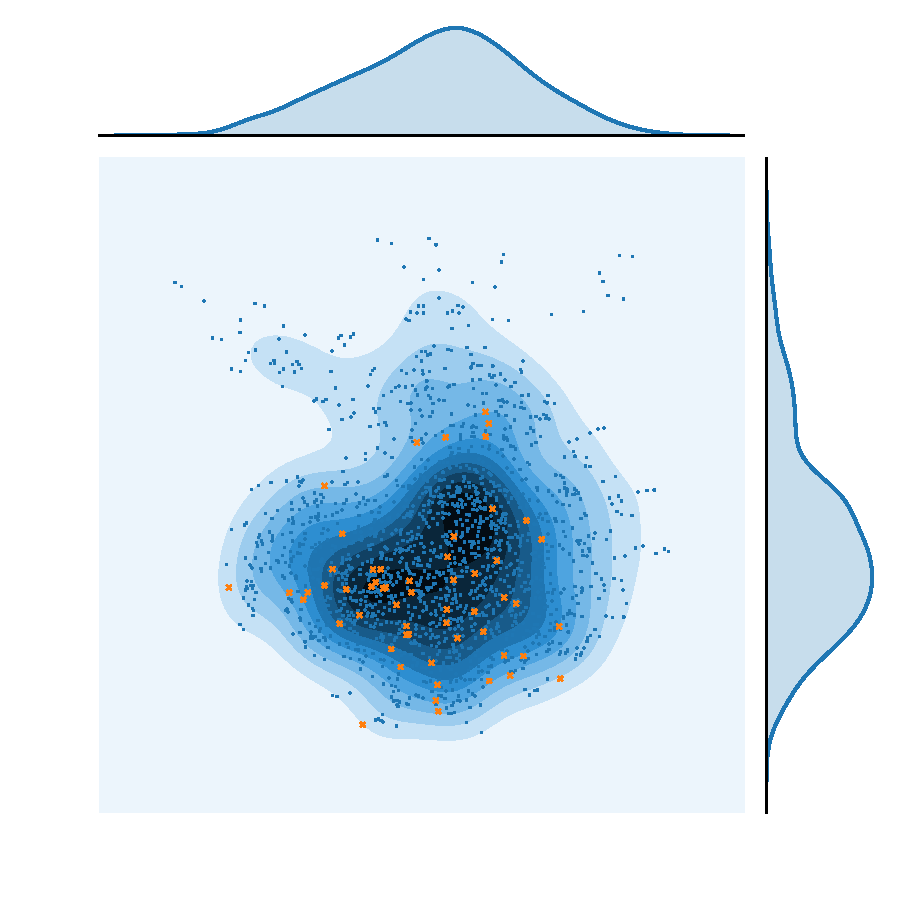
\includegraphics[width=\textwidth,angle=90]{figures_c1/layout/yfan_aphh.pdf}
         \caption{Yifan Hu}
         \label{fig:yfan}
     \end{subfigure}
     \begin{subfigure}[b]{.49\textwidth}
         \centering 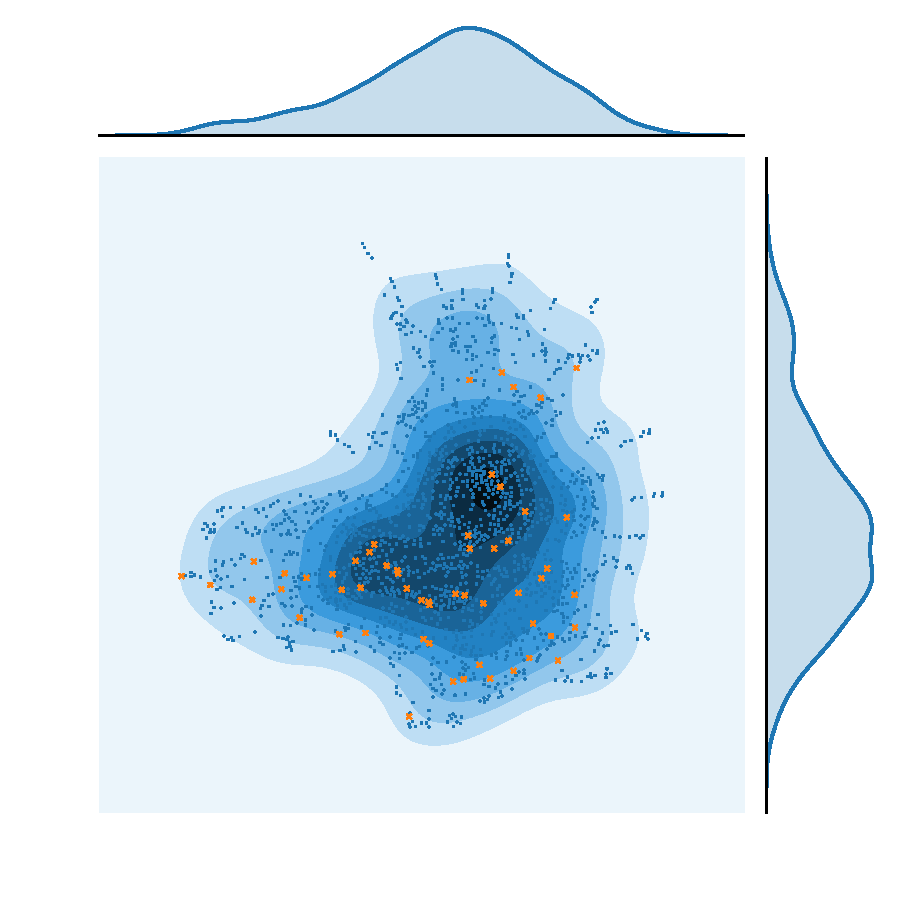
\includegraphics[width=\textwidth,angle=0]{figures_c1/layout/fa_aphh.pdf}
         \caption{Force Atlas 2}
         \label{fig:fa}
     \end{subfigure}
    \begin{subfigure}[b]{.49\textwidth}
         \centering 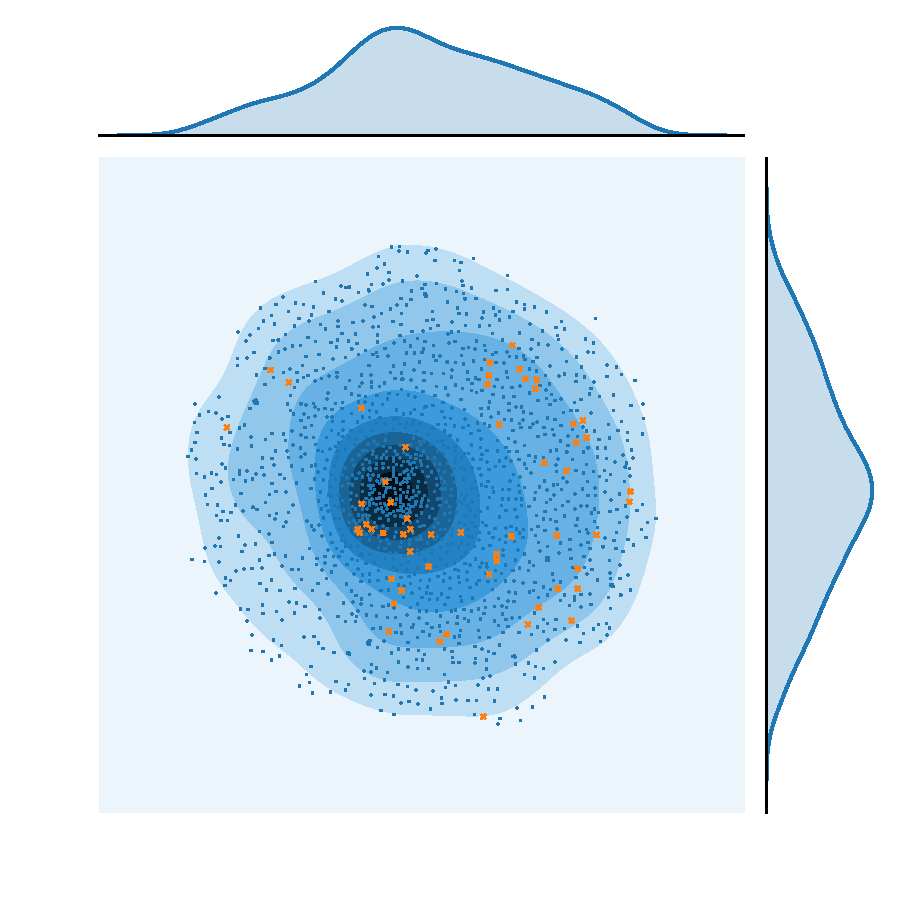
\includegraphics[width=\textwidth,angle=-180]{figures_c1/layout/oo_aphh.pdf}
         \caption{OpenOrd}
         \label{fig:oo}
     \end{subfigure}
         \begin{subfigure}[b]{.49\textwidth}
         \centering 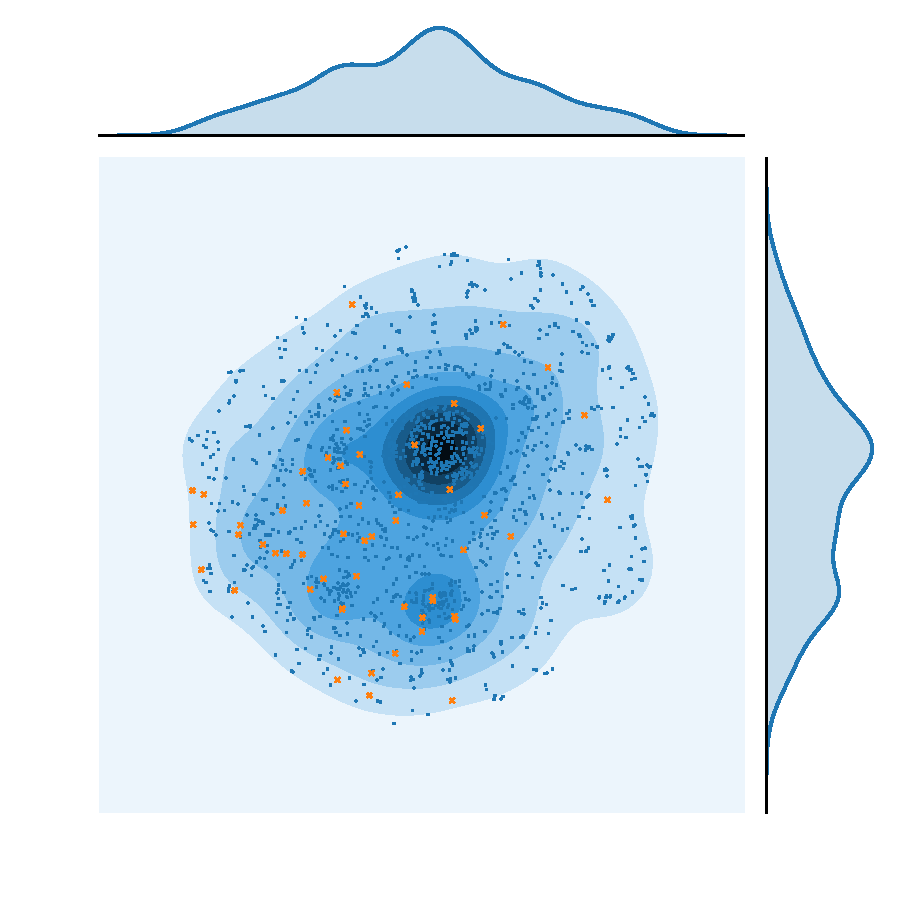
\includegraphics[width=\textwidth,angle=-90]{figures_c1/layout/tsnet_aphh.pdf}
         \caption{tsNET}
         \label{fig:ts}
     \end{subfigure}
      \hfill
        \caption{ }
        \label{fig:densitycompare}
\end{figure}

Here small localised areas of higher density, surrounded with sharp changes in density (shown by the contour lines) is preferable. Such a distribution would highlight the modularity of a graph and allow for the distinction between groups of species with many reactions between them, but few in another group. Graphs with a high homogeneity can be determined through the use of $x$ and $y$ kernel density plots. Here a homogeneous graph will have a uniform distribution across both axes. However, as we also wish to locate regions of chemistry with high modularity (clustering), a uniformly distributed graph would not suffice. Instead, we look for a near-uniform oscillatory distribution with an equal amplitude for each peak and trough. Using these criteria the Mercator (\autoref{fig:merc}b), tsNet (\autoref{fig:ts}) and Force Atlas (\autoref{fig:fa}) score the highest, with OpenOrd and Yifan containing a gaussian-like distribution across both axes which is conducive to producing a hairball. 

Next, we apply prior knowledge about the graph we are trying to visualise. Here we know that the chemistry within a mechanism is determined by the oxidation of a set of primary emitted VOCs. It, therefore, follows that for an ideal graph layout, each primary emitted species should belong to its area of high density, and not entwined within the hairball. Immediately this notion eliminates the Yifan Hu (\autoref{fig:yfan}) and Mercator (\autoref{fig:merc}b) layouts since these both contain a high density of primary emitted species (orange crosses) within a single dense region. Using this criterion, the tsNET graph (\autoref{fig:ts}) provides the best representation, followed by the OpenOrd and ForceAtlas layout. 







\subsection{Node Density}\label{sec:nodedensitya}
Having explored the spatial distribution of nodes within a graph, it is important to determine which layout produces the best node density variation not only across the $x$ and $y$ directions. Here we desire a degree of regular anisotropy to produce `clusters' of densely connected nodes sparsely separated in space. To calculate the distribution between dense and sparsely packed nodes, it is possible to use Voronoi tesselation. Here each node acts as a seed, and the plane is partitioned into a series of $n$ cells, where $n$ is the number of nodes. Each cell or polygon is calculated such that a polygon boundary is determined by all the points which lie closer to its source seed than any other- mathematically this would be defined as the perpendicular bisectors of the lines between all points. The result is somewhat similar to a box full of bubbles, where each bubble fills the largest area it can before meeting another. Next, the area of each polygon is calculated and saved to produce a dataset representative of the complete density distribution between nodes. Here larger areas represents a species with distant neighbours (spatially), and a small one, an area of high density. The method of using vernouli teselation for the calculation of density has been used in the study of neurones \citep{neurone} and areas of fixation when viewing images \citep{fixation}. 
The last part of this process involves colouring the based on the normalised polygon area values and plotted within \autoref{fig:vornoicompare}. This allows for the clear location of layouts with high isotropy (\autoref{aoo},\autoref{ats}), which only contain many cells of a similar size, and consequently only exhibit a slight colour gradient difference between points. Although such layouts are spatially efficent, they do not reveal any additional information about the network structure. 
The colouring can also reveal the the spatial modularity of the graph. Here it is shown that the mercator, despite having a high $x-y$ node distribution, still contains large areas of unoccupied space due to its non linear density distribution. Under this criterion the ForceAtlas and YifanHu layouts (\autoref{afa},\autoref{ayfan}) perform best, with distinct modules of high density appearing to be distributed across the graph. 



\begin{figure}[H]
     \centering
    \begin{subfigure}[b]{.49\textwidth}
         \centering 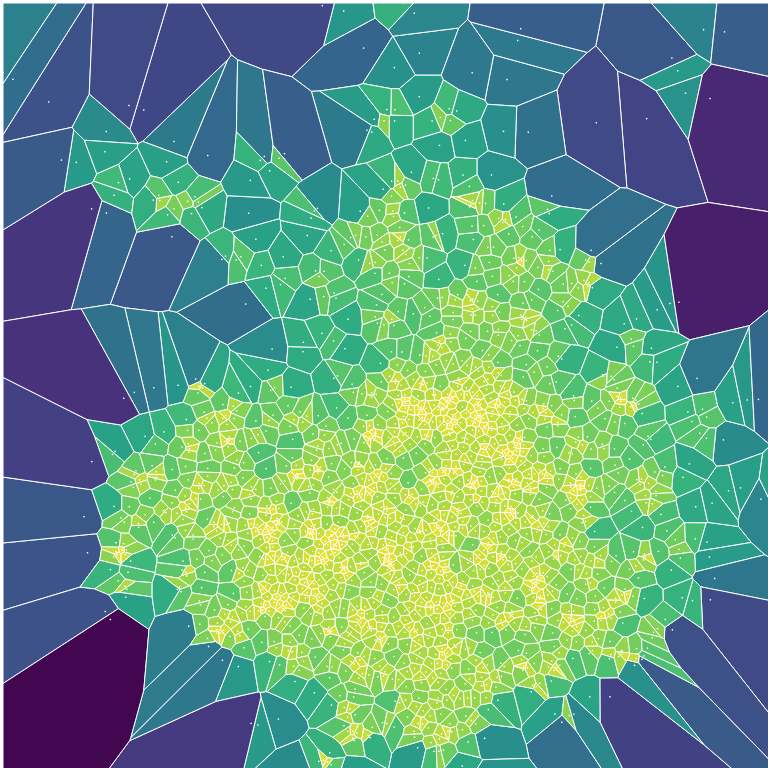
\includegraphics[width=\textwidth,angle=90]{figures_c1/area/fill_yfan_aphh.png}
         \caption{Yifan Hu}
         \label{fig:ayfan}
     \end{subfigure}
     \begin{subfigure}[b]{.49\textwidth}
         \centering 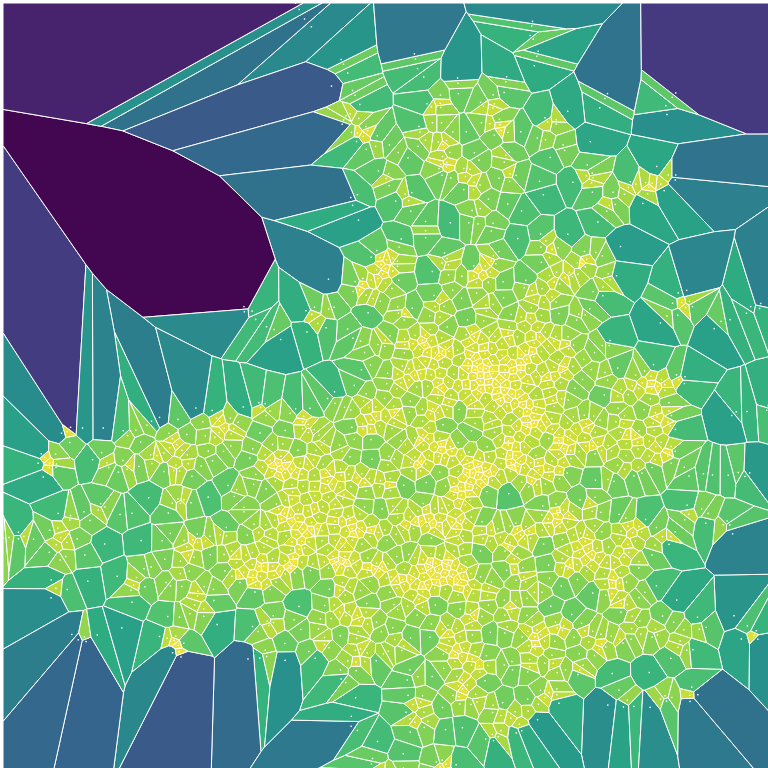
\includegraphics[width=\textwidth]{figures_c1/area/fill_fa_aphh.png}
         \caption{Force Atlas 2}
         \label{fig:afa}
         \end{subfigure}\\
     \begin{subfigure}[b]{.49\textwidth}
         \centering 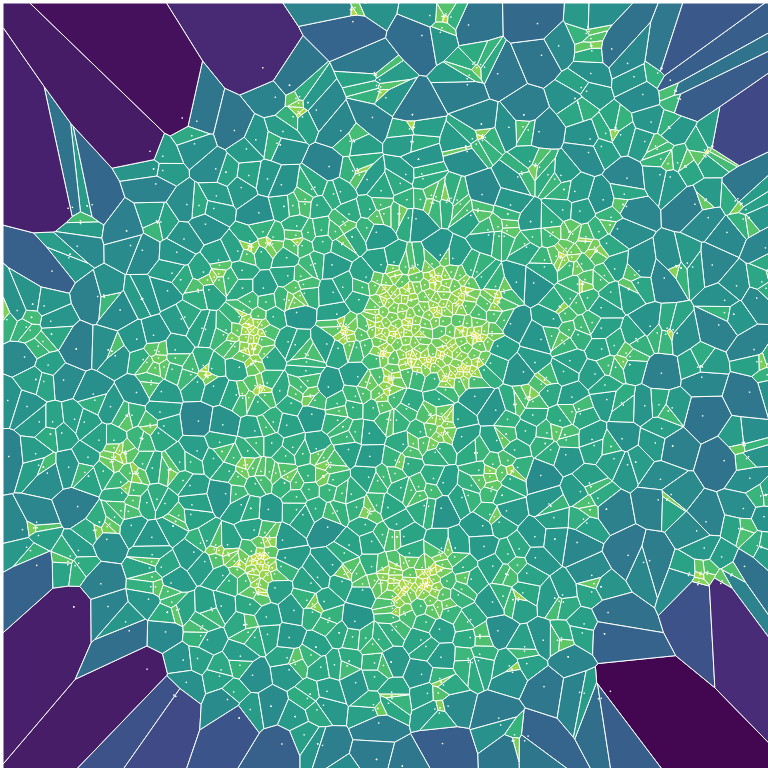
\includegraphics[width=\textwidth,angle=-90]{figures_c1/area/fill_tsnetloc.png}
         \caption{tsNet}
         \label{fig:ats}
     \end{subfigure}
    \begin{subfigure}[b]{.49\textwidth}
         \centering 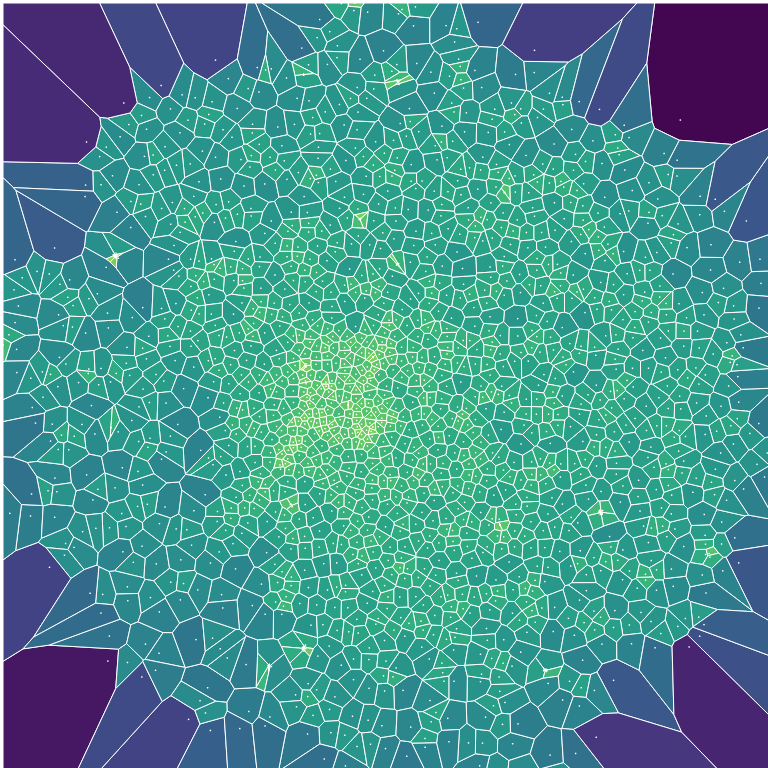
\includegraphics[width=\textwidth,angle=-180]{figures_c1/area/fill_oo_aphh.png}
         \caption{OpenOrd}
         \label{fig:aoo}
     \end{subfigure}\\
     \begin{subfigure}[b]{.49\textwidth}
         \centering 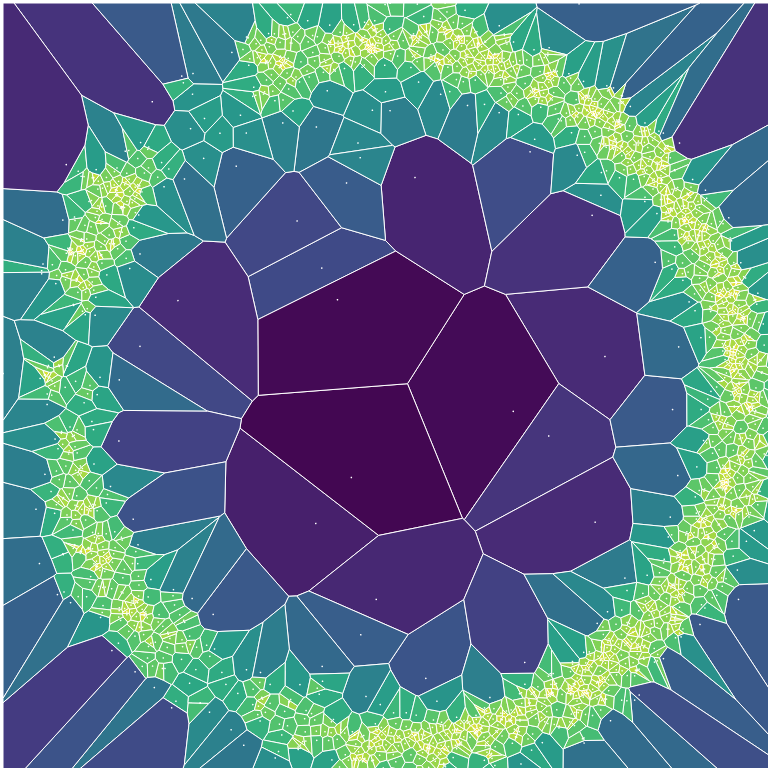
\includegraphics[width=\textwidth,angle=0]{figures_c1/area/fill_mercloc.png}
         \caption{Mercator}
         \label{fig:amer}
     \end{subfigure}

        \caption{Comparing the density of nodes for different layouts using voronoi cell areas.}
        \label{fig:vornoicompare}
\end{figure}

\subsection{Mathematical Analysis And Layout Selection}
In addition to the qualitative approach through visualisation, it is also possible represent the polygon areas for each layout in the form of several boxplots, \autoref{fig:abox}. The interquartile (IQR) range for each layout represents the range of polygon areas. A large IQR signifies a greater distribution between low and high density  areas. 
In addition to this we are interested in having a higher ratio of smaller area polygons to larger ones. Within the boxplot, this would be represented by having a median which is closer to, or approaching the $25^{th}$ quartile ( the lower box boundary).

\begin{figure}[H]
\centering 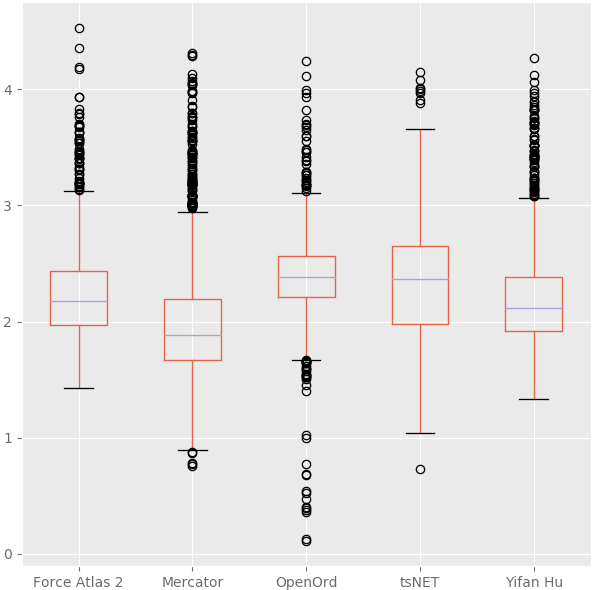
\includegraphics[width=\textwidth]{figures_c1/area/log10layoutbox.png}
\caption{Voronoi $\log_{10}$(Area) BoxPlot for all plots in \autoref{fig:vornoicompare}}
\label{fig:abox}
\end{figure}


Applying these citerions to \autoref{fig:abox}, shows Mercator to provide the best result. However in combining this with our previous observations, is is noted that although the ratios approach our ideal range, its radial shape is not conducive to the general represenation of modularity within a network. The layout with the largest IQR is produced using tsNET algorithm. Although this produces a well distributed algorithm, its inability to handle directed edges and high median rule it out as a possible candidate. The OpenOrd layout can reduce the number of hariballs within a graph through the use of simulated annealing and edgecutting, however it is also this property which in this case has resulted in a homogenious isotropic node distribution (as shown by the small IQR with a sizeable median value). Unfortunately this is not shown as the most effective at hilighting the underlying structure of the chemical mechanism. 

This leaves the Force Atlas 2 and Yifan Hu layouts. Out of these the Yfan Hu layout fares better with regards to the box plot, yeilding an overall lower box, with a similar IQR and median ratio. Here its lower median suggests more high density nodes, with a similar distribution to the Force Atlas. This makes sense, since the two algorithms share many similarities, however once again the inability to handle directed edges makes it unsuitable for our application. 

This leaves the Force Atlas as the preffered layout for the visualisation of chemical mechanisms. Its directed nature coupled with intuitive design make it applicable and easy to explain, whilst still maintaining an ability to produce a clear representation of any underlying structure. In addition to this, its more uniform spatial distribution (\autoref{sec:nodedist}) makes it a better candidate than the Yifan Hu graph, which scored the highest in the boxplot test. 













\section{Graph Semantics}\label{semantic}

Deciding the correct semantic representation for a visualisation is often just as important as the selecting the correct syntatic style. Semantic features are often applied post generation \citep{aestheticsgraphvis} and have uses in the encoding of additional information and clarifying any results within the data. As a means of achieving both an aesthetically pleasing outcome, and an easy to understand visualisation, we must first consider what features we, or the reader, are most interested in. Once this has been decided, we begin to explore various methods for representing them. 

\subsection{Limitations}

When selecting visualisation semantics, there are several limitations that we must consider. 

\paragraph{Visual}
When it comes to Visual analytics the most significant bottleneck is due to the resolving power of the eye - this is known as an acutie. Acuities are a measure of the angle of an observed object with the viewer's eye using arcs (one arc equates to $\frac{1}{60}^{th}$ of a degree). This provides a unit of measurement for the total amount of information density we can feasibly perceive \citep{ware}. 

 In ophthalmology there exist four types of  acuities: 
\begin{itemize}
\item[-] \textbf{detection}: The smallest size an object can be whist still being shown
\item[-] \textbf{recognition}: The smallest size an object can be to be recognised
\item[-] \textbf{resolution}: The smallest distance between two objects before they begin to merge
\item[-] \textbf{localization}: The smallest amount of visual change that can be measured between two objects
\end{itemize}

These provide a set of considerations which may be used to assess a visualisation. Depending on what encoding we use, it is possible to improve/hinder the readers ability to percieve information, \autoref{acuity}. An example of this would be that for a Macbook Pro retina screen\footnote{A retina screen, is half the maximum possible resolution of the human eye at a 30cm distance. Additionally the operating system interpolates in sets of 4 pixels, such that the image displayed may not be at full resolution.}, where at 87 pixels/cm\footnote{at 57cm from the screen} we can display at most 2 million resolvable nodes. If we wished to add links between nodes, the total resolvable items is reduced to one million
\citep{ch10}. 

\begin{figure}[H]
\begin{center}
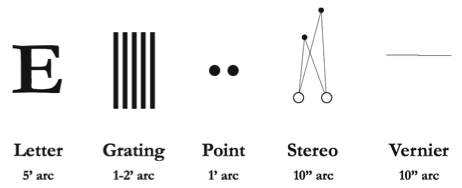
\includegraphics[scale=.6]{figures_c1/acuity.png}
\end{center}
\caption{Important acuities in visualisation, Source: \citep{ch10,ware}}\label{acuity}
\end{figure}


\paragraph{Cognitive}
Although it may be possible to distinguish 1 million nodes and links visually, interpreting and understanding these presents another problem. The visual thinking laboratories \citep{vt}, have a range of publications exploring how presentation can improve though, cognition and communication between info-graphic and reader. \citep{OpenVis}, explains that the time required to interpret a visualisation is directly related to the encoding used to hi-light the data within it. Also problems of `intentional blindness' and misinterpretation are problems which are often occurred with poorly thought out encodings.  

In considering the cognitive load of a visualisation \citep{emotional} provides a list of three categories which should be explored:


\begin{itemize}
\item[1.] Firstly we have the visceral level, a subconscious process where decisions are made rapidly based on sensory inputs to the body. 
This is usually due to our inherent ability to locate patterns and changes due to semantic properties which shift the focus of the user.  

\item[2.] Next follows the behavioural level (mostly subconscious). These are often learn reaction to changes noted as part of the visceral level. Here reactions may be honed on and influenced by past experiences and events. 

\item[3.] Finally we reach the reflective level. Here the user collates all sensory input from the previous two levels and makes an informed conclusion about the underlying data. Conclusions drawn here can be used to bias the methods used within the behavioural level in future events. 
\end{itemize}

\paragraph{Technological}
In addition to human limitations, there may be restrictions due to the medium a visualisation is created/presented on. In addition to monitor resolution issue earlier, much scientific research is constrained by the size, resolution and colour quality of the presentation mediums used for talks, printing or posters. \citep{ware} explains that a printer capable of producing 1200 dots per inch squared, can only do this for black/white binary images. If for instance 256-greyscale is used, the resulting resolution is then at-least 10 times smaller. This is because printers a Monet style approach to create shading and colour. It therefore follows that at full CYMK, the output resolution will be worse. 

It is also essential to have a graph fitting the same overall shape of the canvas on which it is presented \citep{graphmetnew}. This not only makes optimal use of any space available, but also reduces the visual complexity as it minimises the number of distinct shapes available to the user. 




 




\subsubsection{Node Encoding}
Within a graph, the nodes represent the set of items we are exploring. Each of these often contain a multitude of features and properties relating directly to them, be it the user details for a retail/fraud network, or the chemical composition and concentration of a species in the MCM. Features of a node describe and additional properties and may be used to determine its interaction with other nodes\footnote{This is further explored in Chapter 4} \citep{protocol}. It is for this reason that graph convoluted neural networks \citep{t2gcn}, require a  `feature matrix' describing each node, in addition to the network structure and edge weightings. Within a visualisation, a node may be represented in a range of ways. 



\begin{figure}[H]
     \centering
     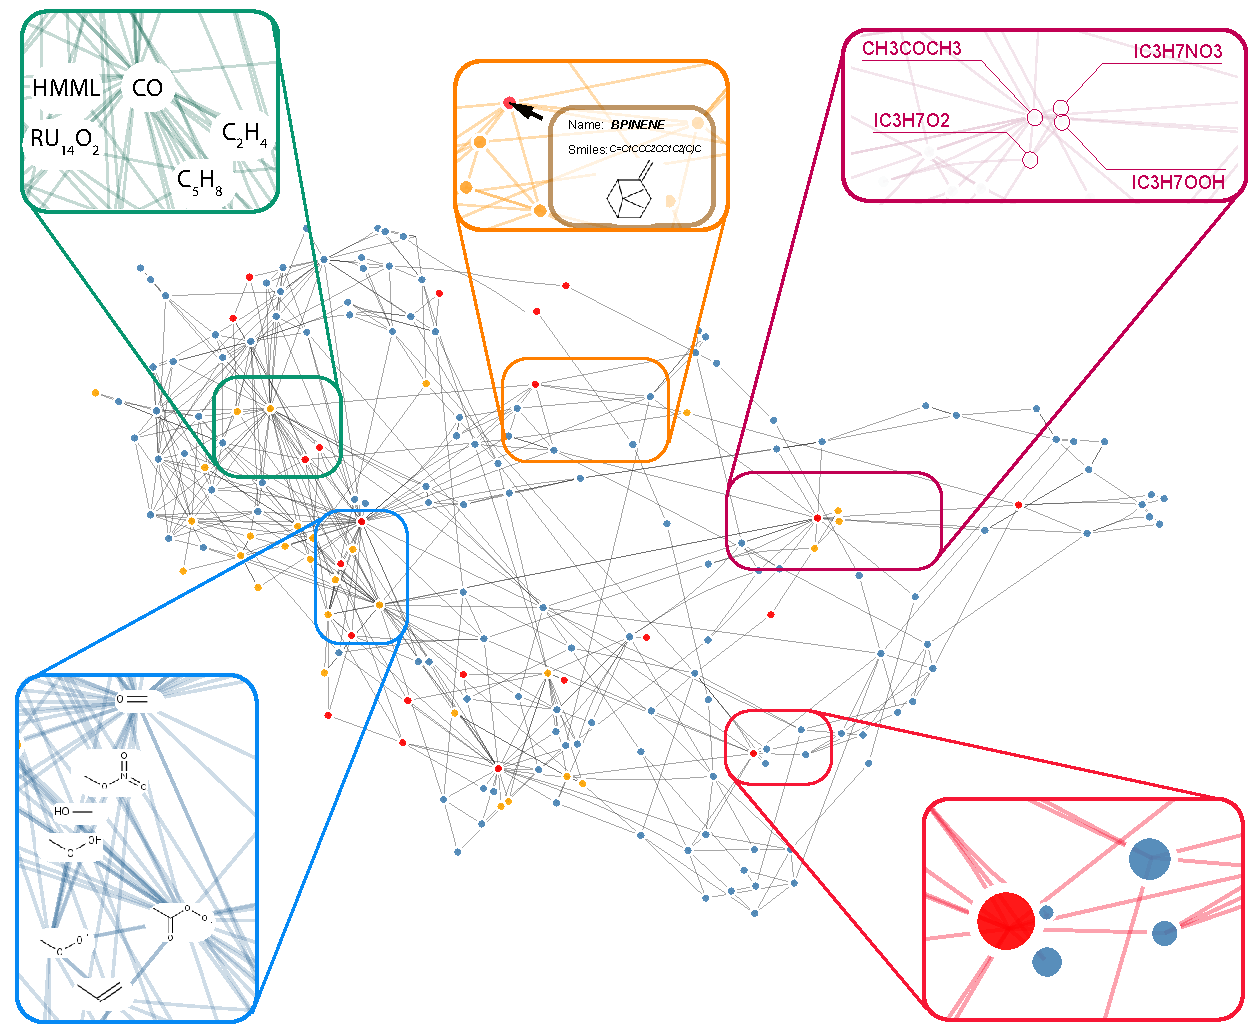
\includegraphics[width=\textwidth]{figures_c1/NODES_001f3d-00775b-ff9000-f71735-c10053.pdf}
        \caption{\textbf{A graph showing 5 different node encoding methods.} These are Circle Atrributes (red), Chemical structure (blue), Species Name (green), External Labels (maroon) and interactive selection (orange). The network shows the Common Representative Intermediate species \citep{cri} mechanism. Node colours represent primary emitted VOCs (red), MCM species (orange) and lumped CRI-only species (blue).  }
      \label{fig:nodestyle}
\end{figure}





\paragraph*{\color{c4}Circle Attributes}



The simplest of these range from the use of colour, shape, size, thickness and stroke (outline) to indicate a group. Here it is possible to provide information such as a species concentration based on its size, its importance with its colour, its degree with its opacity and its category with its stroke colour \citep{colourb,rightness}. Such descisions depend on what properties you are trying to show. For instance red species in \autoref{fig:nodestyle} are primary emitted VOCs, orange species exist between both the MCM and the CRI (see figure caption) mechanism, and blue ones are lumped species which do not appear as part of the MCM.  


\paragraph*{\color{c1}Chemical Structure}
Traditional chemical diagrams use the chemical structure to depict the types of reaction that occur , \autoref{fig:butane}. This make it intuitive to extract information about functional group and bond changes within species. Such a method of representation, is indeed useful, however when visualising hundreds, if not thousands of nodes on a page, it results in occulsion, or labels too small to resolve visually. 

\paragraph*{\color{c2}Species Name}

Much like the chemical structure, a species name is proven useful in explaining to the user its chemical properties (often due to prior knowledge, or the ability to look this up). Unfortunately since names have differing lengths, this can cause problems, especially with large numbers of closely located nodes. A solution to this may be to adjust the font size to fit in within the circle radius of the node. However this does come with its problems - for instance tiny nodes may have text smaller than a pixel, or the misleading notion that longer names are less important, since they are represented by a smaller font. 


\paragraph*{\color{c3}Interactivity}

Ben Shneiderman's famous mantra goes: \emph{`overview first, zoom and filter, details on demand'} \\ \citep{mantra}. This goes hand in hand with the philosophy used within the design of an interactive visualisation.

For complicated systems, interactivity plays a vital role in unraveling complexity and reducing clutter \citep{interaction1}. It allows the user to actively query only the items that they are interested in whilst still displaying all the information in a single location \citep{oneplace}. 

A comprehensive list of all available interaction types and styles are provided in \citep{ch6}. Some examples of interaction are:\\ 

\begin{table}[h]
    \centering
    \begin{tabular}{p{.45\textwidth}p{.45\textwidth}}
\textbf{Hi-lighting}
\begin{itemize}
\item Hovering
\item Brushing and Linking
\item Magic Lenses (see hidden objects)
\end{itemize}
&
\textbf{Visual Structure-Level Interaction}
\begin{itemize}
\item Selection
\item Changing layout/mapping attributes
\item Changing representation
\end{itemize}
\\
\textbf{Navigation}
\begin{itemize}
\item Pan / Zoom
\item View Distortion (fisheye)
\end{itemize}
&
\textbf{Data Level Interactions}
\begin{itemize}
\item Adding / Filtering
\item Search / Query
\end{itemize}

\end{tabular}
    \caption{\textbf{A selection of interactive methods.}}
    \label{tab:interactive}
\end{table}

\begin{figure}[H]
     \centering
     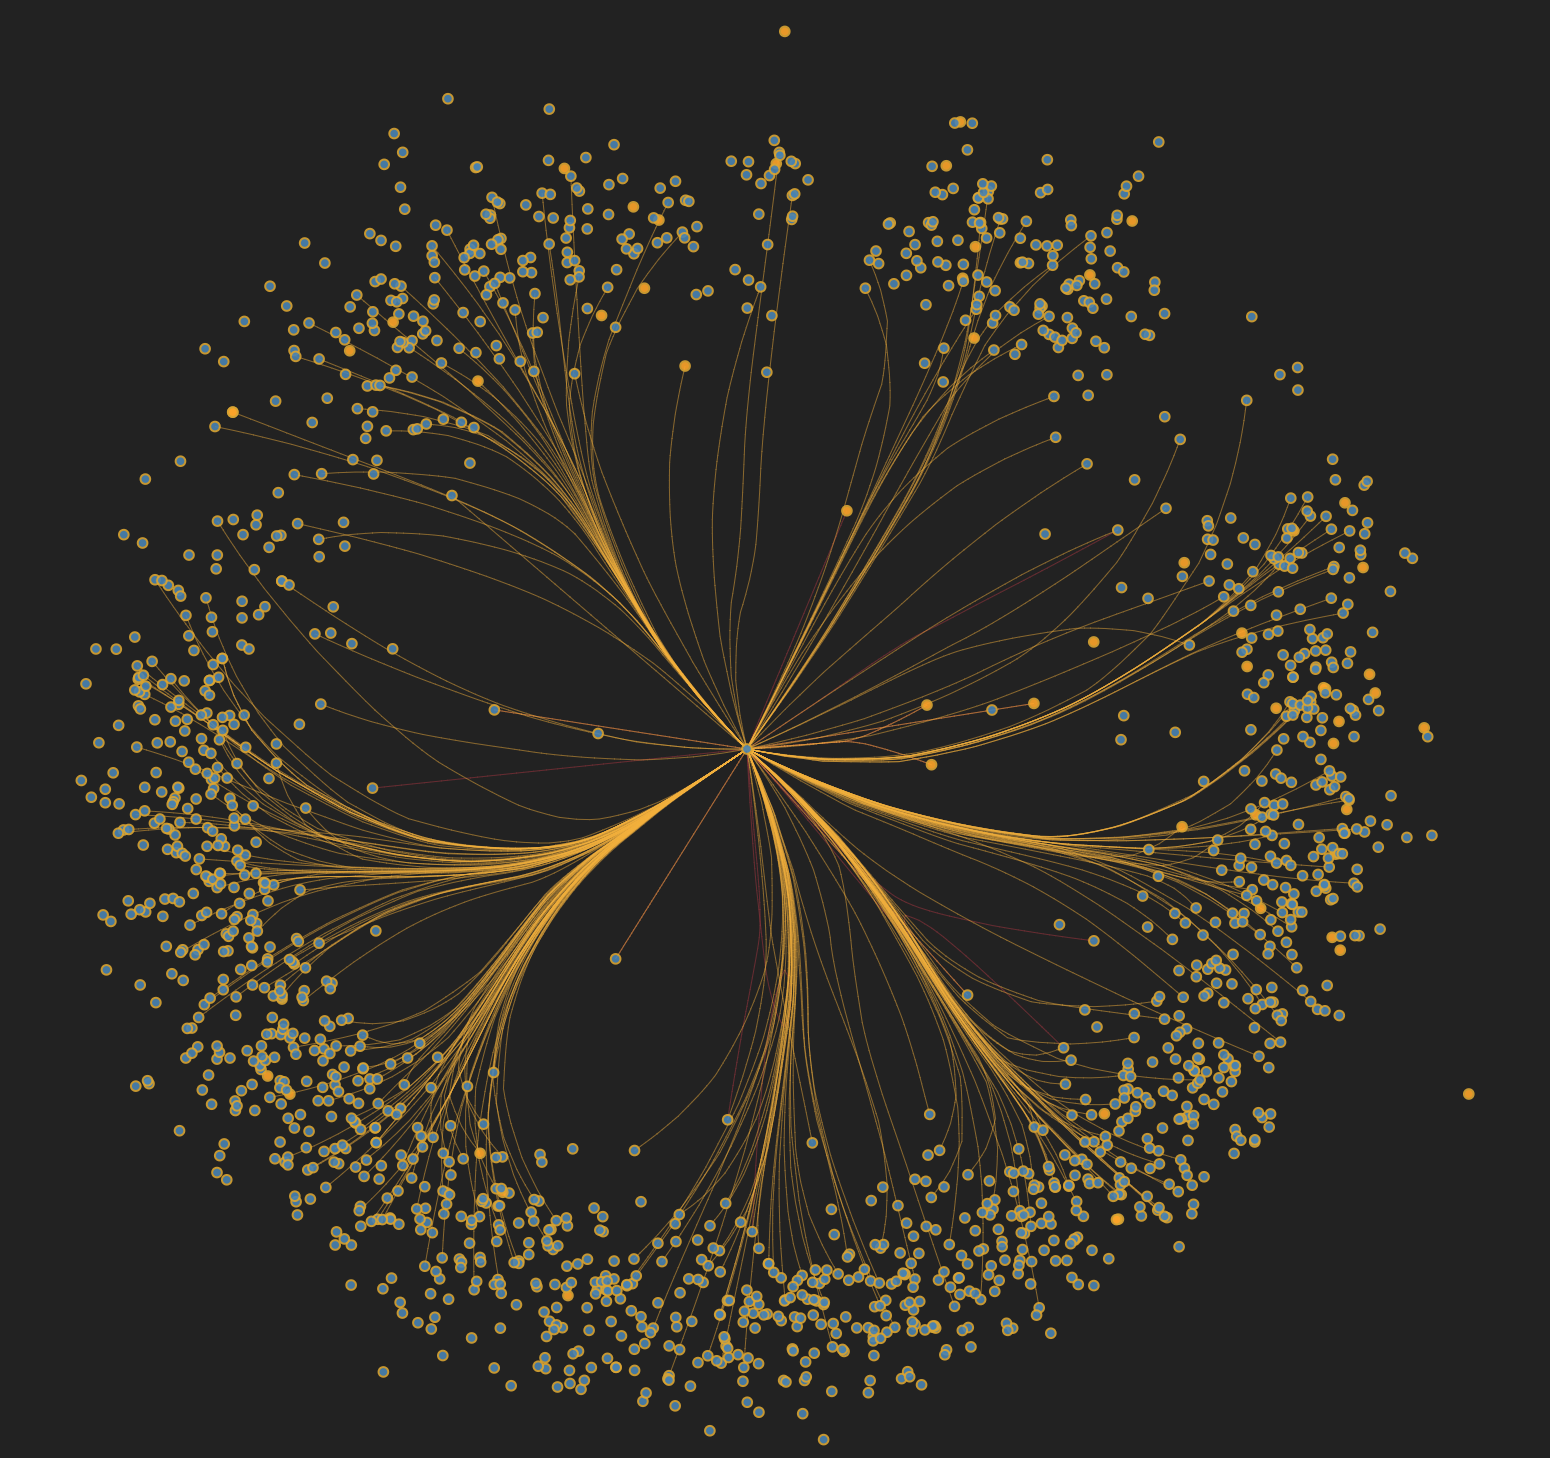
\includegraphics[width=0.7\textwidth]{figures_c1/layout/CObranches.png}
        \caption{\textbf{Using mouseover edge-selection to hilight all links related to a node. } This figure shows how in using interactivity it is possible to reduce clutter and filter the information presented by a densely populated graph. In this case the mercator projection (\autoref{sec:merc}) is used, with reactions relating to Carbon Monoxide (centre) hilighted. Orange lines represent reactions producing CO whist the red (some of which may be hidden) are of reactions with CO.  }
      \label{fig:tooltip}
\end{figure}

\paragraph*{\color{c5}External Labeling}
In cases where interactivity is not possible, such as papers, books and this thesis, an alternative approach to data selection has to be employed. Here nodes which are central to the explanation of a certain point are filtered by the author, and displayed through the use of external labels. It is found that having links at 45 and 90 degree angles (such as in transport maps) lead to a clearer layouts and better distinction from the links already within the graph. Automatically generated labels within the thesis are made using \citep{d3annotate}.







\subsubsection{Edge Properties}


Defining the purpose of graph-energy models as: a means for creating a visualisation from which the viewer can infer properties of the data \citep{noack}, it can be shown that this criterion is easily met in small and sparse graphs. However non-planar examples with high edge density (lots of links) can easily result in tangled results with impractical running times \citep{tvg}. In most cases attaining an optimal solutions here seems to be computationally infeasible \citep{nicelyanneal}. This is generally because graphs primarily focus on hi-lighting a specific purpose or following a set of aesthetic heuristics \citep{eyetrack}. 

Butane model 


\paragraph{Muti-variate edges}
Since there are multiple relationships between species, it is important to decide if simplifying the network would be of benefit. Although it is possible to \autoref{fig:multiedge}.. 
this may cause unecessary clutter for larger networks. Instead it is often useful to simplify the graph, and encode the edge properties within the vector object. This allows the user to retreave any additional information by hovering over the edge or connecting nodes, as required. Should the topic of interest require a specific property, then it would also be possible to remove, or hide, all edges which do not contain it. This produces an interactive graphic containing all the required information, as and when needed, without the unecessary clutter of having every reaction shown. 

\begin{figure}[H]
     \centering
     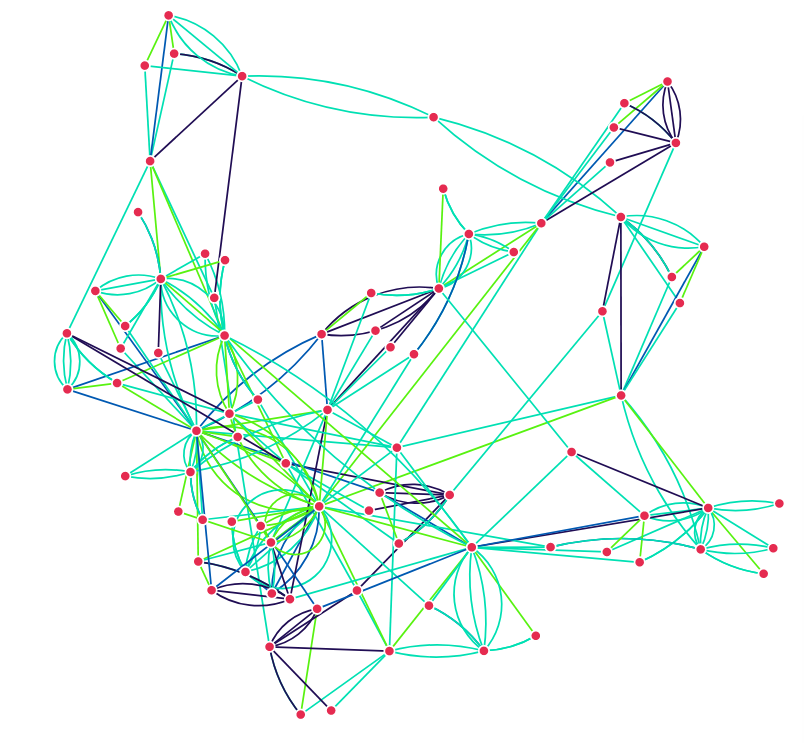
\includegraphics[width=.7\textwidth]{figures_c1/edgetype/multiquadratic.png}
        \caption{\textbf{Multiple edges coloured by type of reaction.} Using the overarching categories of reaction type (see fig wuclan) each type of reaction between two nodes can be visualised using the multi-link format. Photolysis (Bright green), Radical/Other (Amazonite / Teal) Decomposition (Honolulu Blue), RO2(Space Cadet / Purple)}
      \label{fig:multiedge}
\end{figure}

% %
% Photolysis (Bright green), Radical/Other (Amazonite / Teal)
% Decomposition (Honolulu Blue), RO2(Space Cadet / Purple)
% 





\paragraph{Edge Direction}
When using a directional graph it is convention to use arrow heads to represent this. However in high density regions it is often found that arrow heads take up precious real estate in the drawing area \citep{noarredge}. As an alternative, colour and line-type can be used to represent the direction instead. This example can be shown in the routing networks presented by \citep{networkrouting}. One example applicable for chemistry would be the use of dashed lines to represent mono-directional relationships, and continuous lines for bidirectional ones. 








\paragraph{Edge Shape}
Edge shape is essential, as it is the medium we use to represent relationships within a graph. For orthogonal graphs, poly-line curved edges are used to provide a layout which is simpler and easier to read \citep{ortho}. For asymetric graph drawings circular Lombardi-style curves and cubic brezier lines have been used to reduce the clutter in high edge-density drawings \citep{lombardi,bezier}. \autoref{fig:curvededge} shows a selection of different edge types for the Butane MCM subset.The liear network (\autoref{fig:curvededge}a ) consists of straight lines betwen nodes. If a multi-edge graph is required, it is impossible to represent this as all edges between two nodes follow the same path. To improve on this a quadratic arc (\autoref{fig:curvededge} b) can be used. This presents a symmetric representation where each edge is revealed. Finally bezier curves (described below) can be used to show an asymetric representation of the multi-edge graph (\autoref{fig:curvededge}c). Both sets of curved representation rely on a set of control points, allowing the designer to control the curve shape, steepness and asymmetry. 

\paragraph*{Bezier Curves}
Bezier curves are named after Pierre Bezier who used them in the bodywork design of Renault cars in the 1960s \citep{beziermath}. Since then they have been widely used in graphs,computer graphics, font design and animation/interactivity response \citep{bezier,beziermath,beziercomputer}. Bezier curves come in a range of possible dimensions, cubic beziers are the most commonly used within network visualisation. These contain four control points respectively which can be used to determine the shallowness of the curve through design. In general relatively shallow curves are prefered, as these do not introduce unecessary edge crossing or abrupt changes, which have been shown to hinder a users ability to isolate items of interest \citep{ch6graphredability}.


\begin{figure}[H]
     \centering
      \begin{subfigure}[b]{.32\textheight}
         \centering
     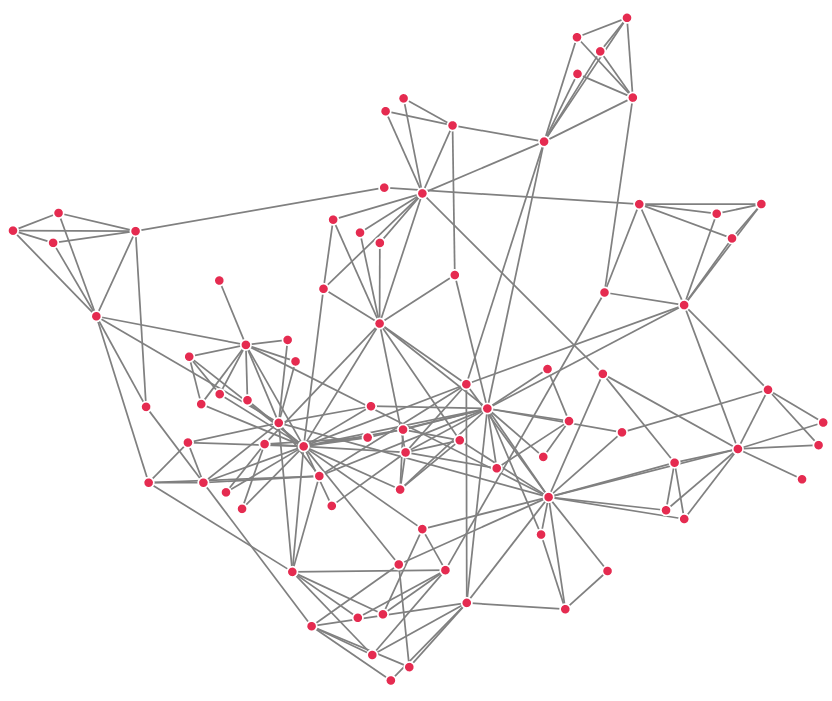
\includegraphics[width=\textwidth]{figures_c1/edgetype/linearsingle.png} \caption{Linear (single-edge)}
     \end{subfigure}\\
    \begin{subfigure}[b]{.32\textheight}
         \centering
     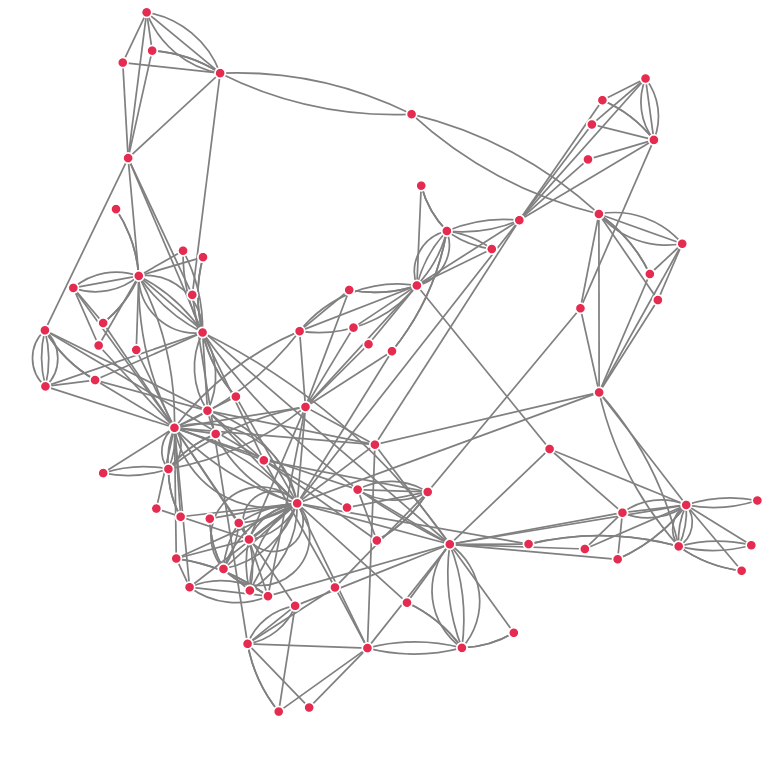
\includegraphics[width=\textwidth]{figures_c1/edgetype/multiquadraticgray.png}
     \caption{Quadratic (multi-edge)}
     \end{subfigure}\\
     \begin{subfigure}[b]{.32\textheight}
         \centering
     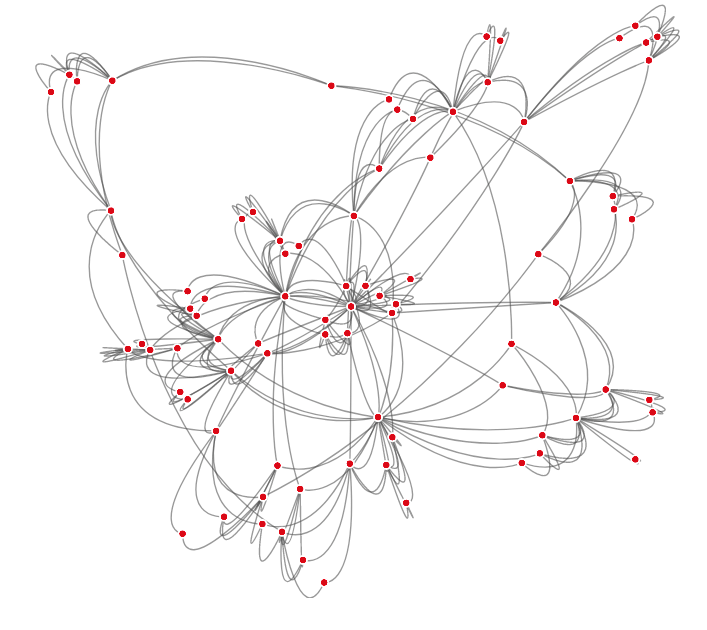
\includegraphics[width=\textwidth]{figures_c1/edgetype/multibeziergray.png}
     \caption{Bezier (multi-edge)}
     \end{subfigure}
        \caption{\textbf{A selection of edge shapes for the butane network.}       }
      \label{fig:curvededge}
\end{figure}








\paragraph{Edge Bundling }
Pioneered by \citep{bundlepioneer}, edge bundling techniques are an effective way to reduce visual clutter. Much like a force graph, edges are represented as a string of lined points. This allows for edges to be pulled together (attracted to one another) and produces a visualisation akin to moving water droplets on a hydrophobic surface. \autoref{fig:edgebundling} shows how in changing the amount of atraction between edges, it is possible to reduce clutter in a visualisation. 


\begin{figure}[H]
     \centering
      \begin{subfigure}[b]{.49\textwidth}
         \centering
     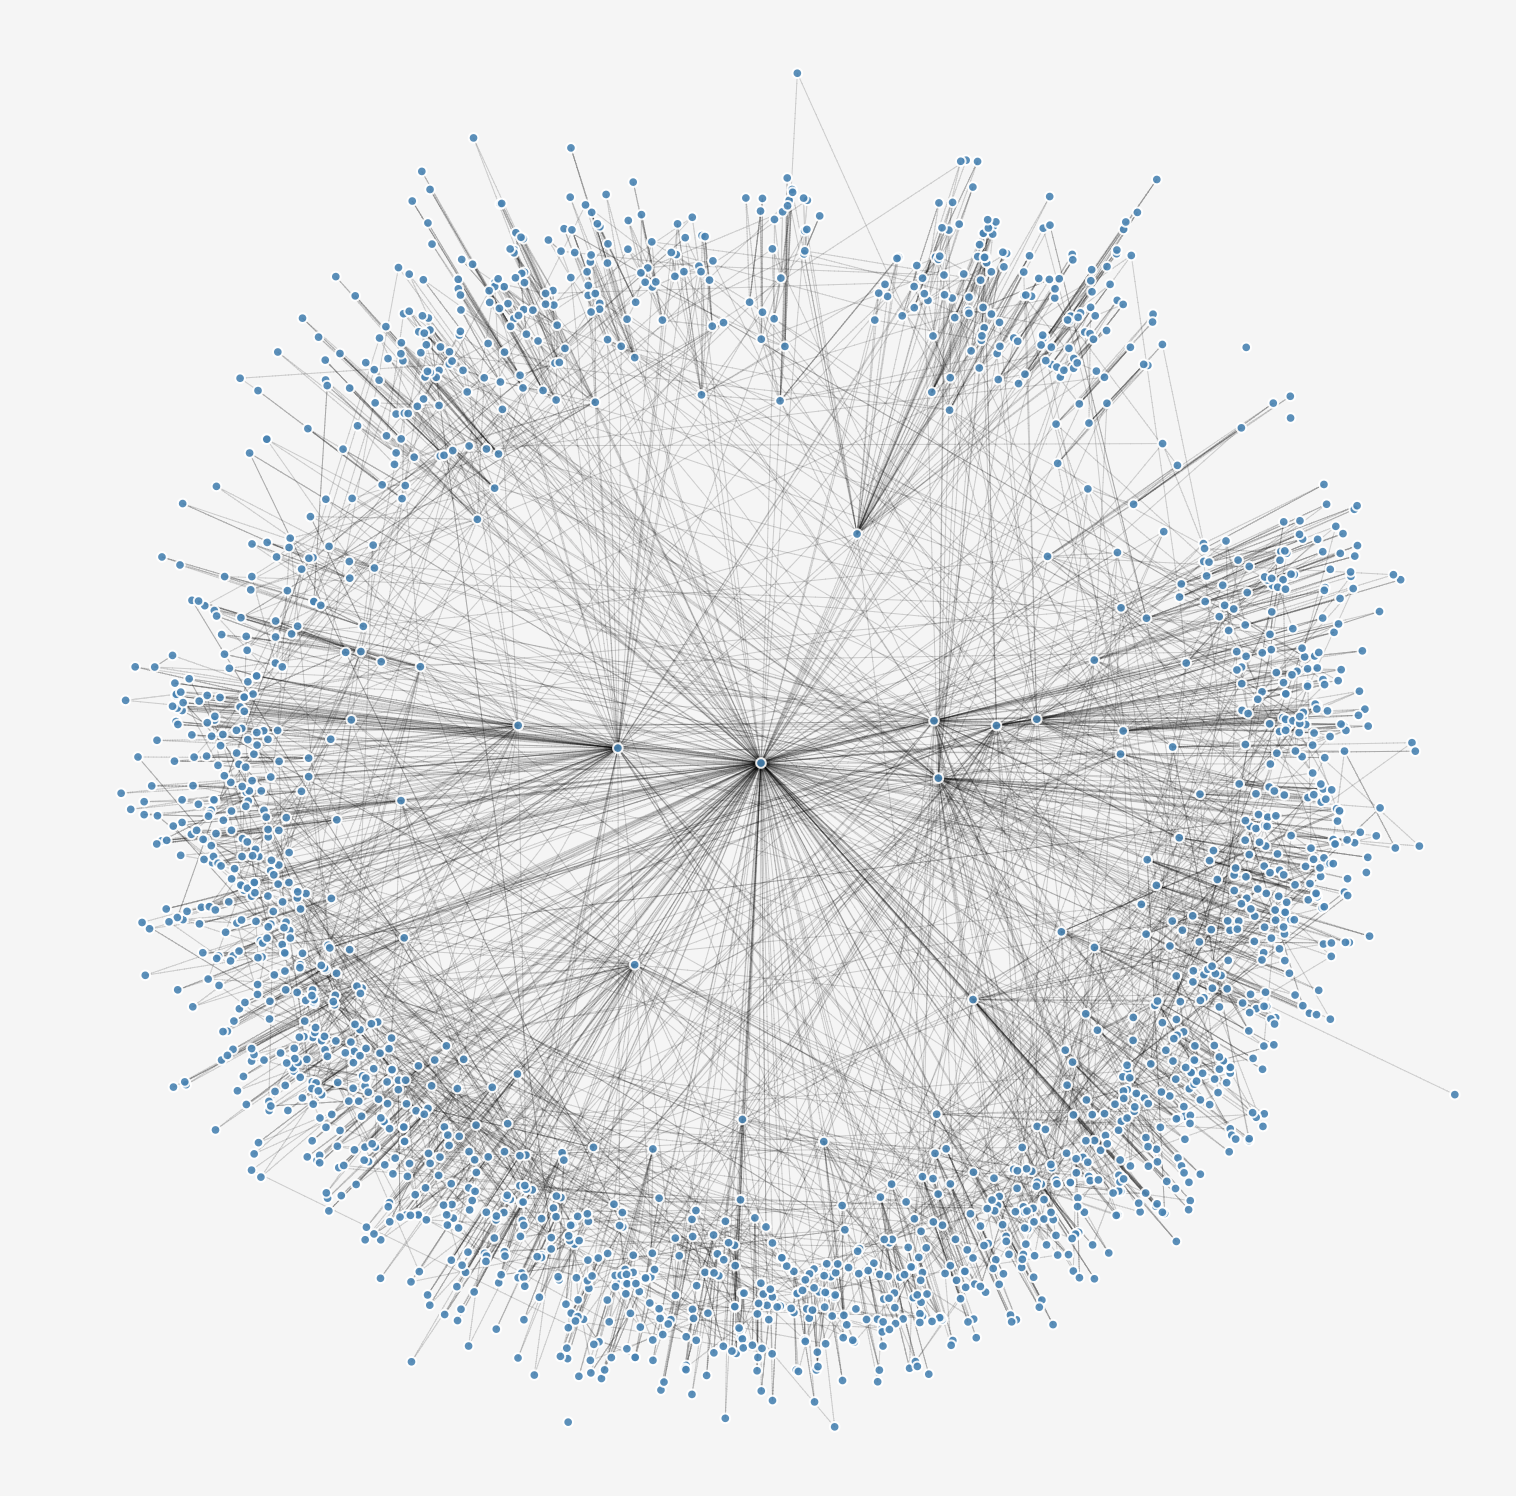
\includegraphics[width=\textwidth]{figures_c1/layout/merc1.png} \caption{$\theta = 1$}
     \end{subfigure}
\begin{subfigure}[b]{.49\textwidth}
         \centering
     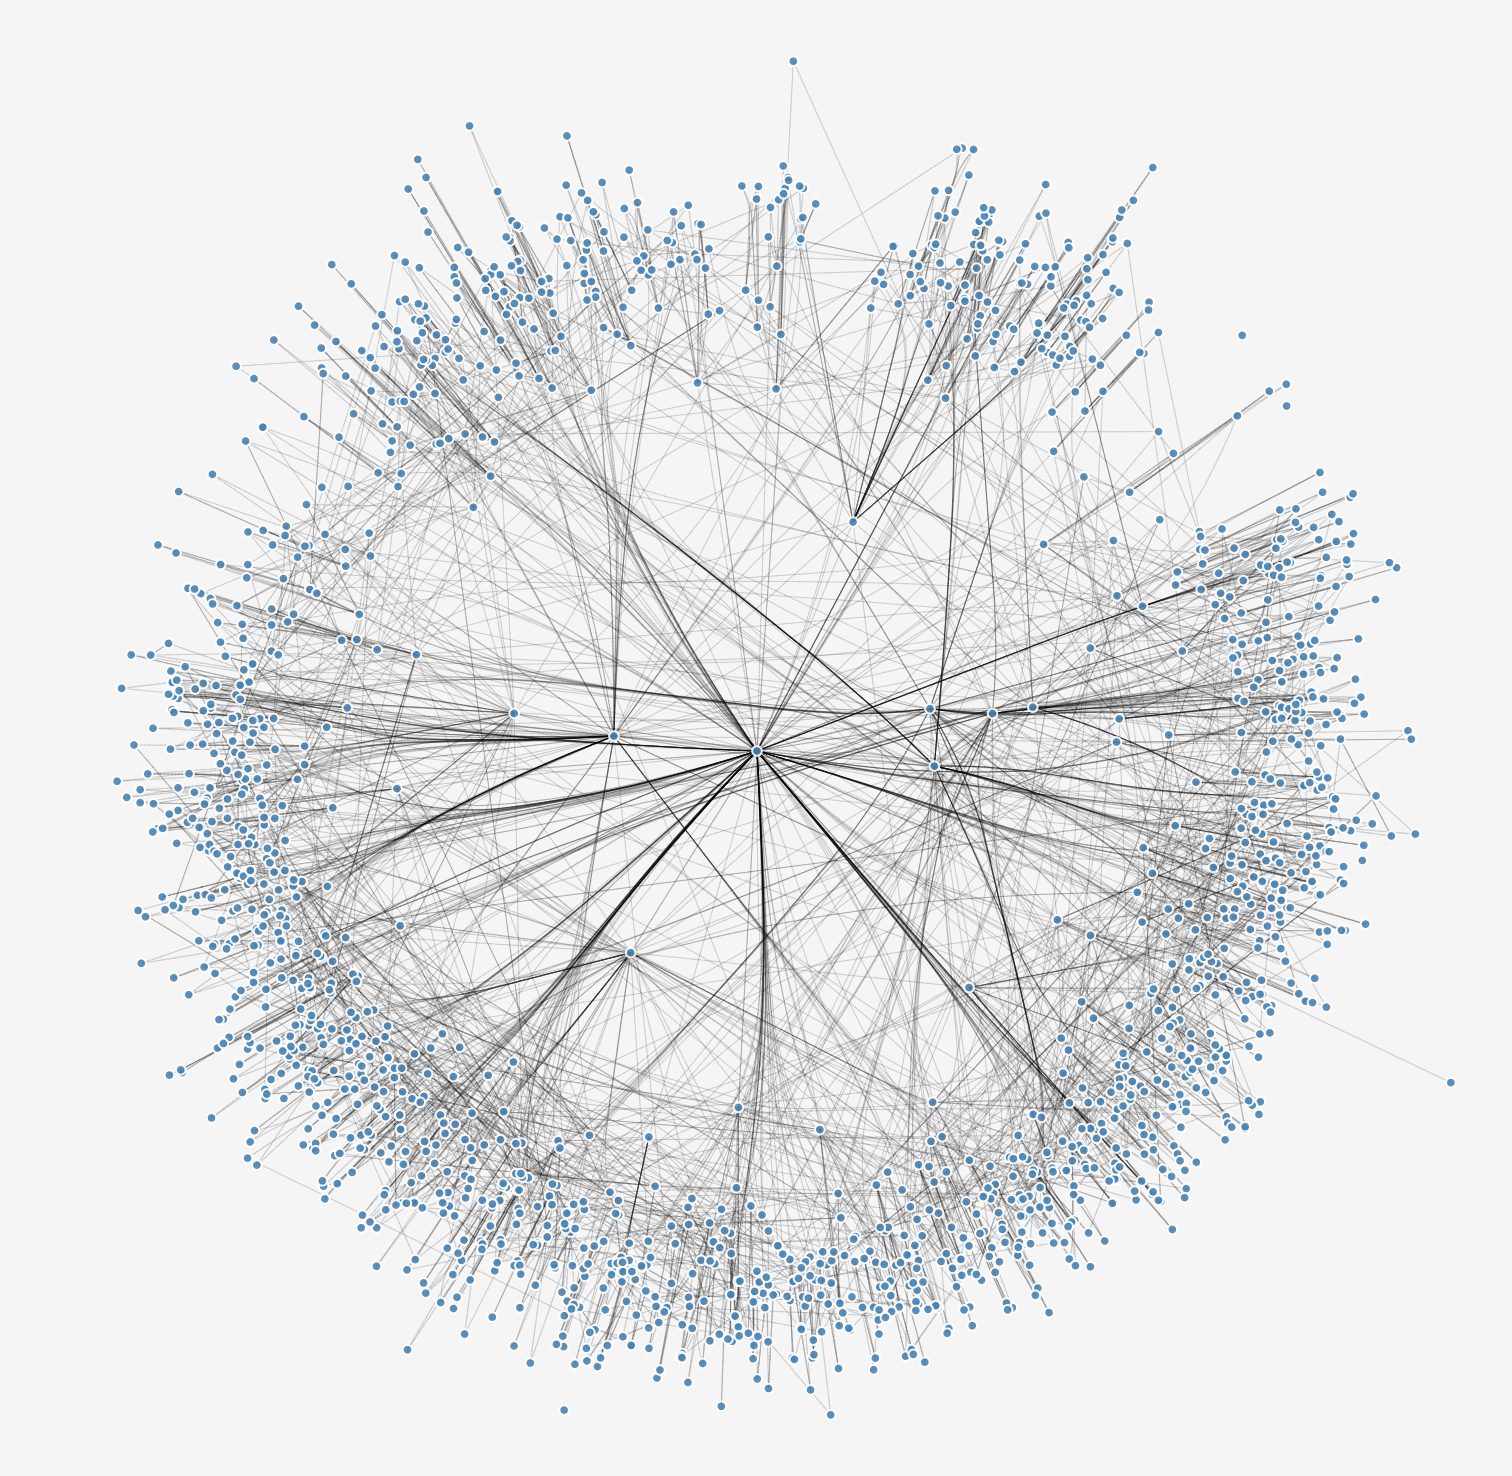
\includegraphics[width=\textwidth]{figures_c1/layout/merc2.png}
     \caption{$\theta = .85$}
     \end{subfigure}
\begin{subfigure}[b]{.49\textwidth}
         \centering
     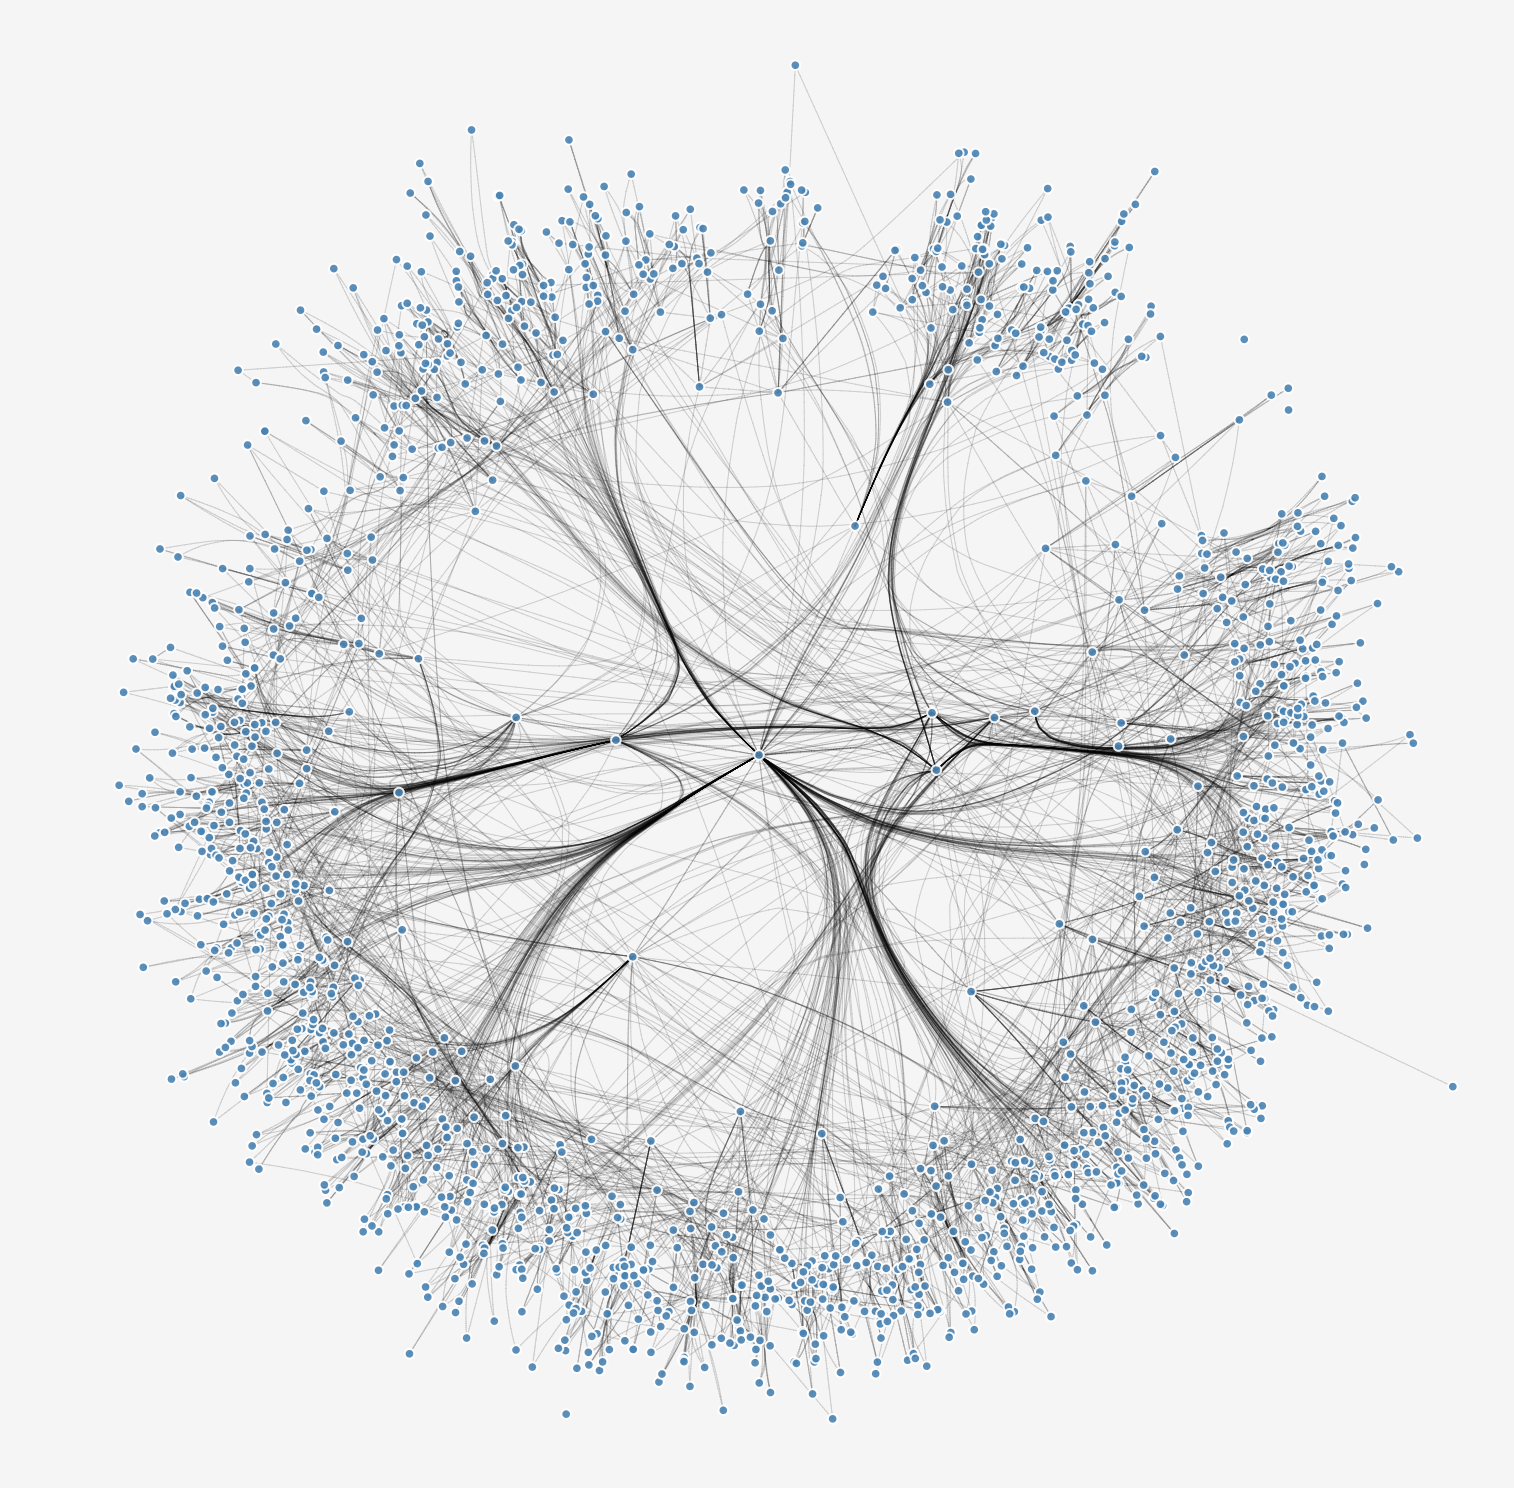
\includegraphics[width=\textwidth]{figures_c1/layout/merc3.png}
     \caption{$\theta = .75$}
     \end{subfigure}
 \begin{subfigure}[b]{.49\textwidth}
     \centering
 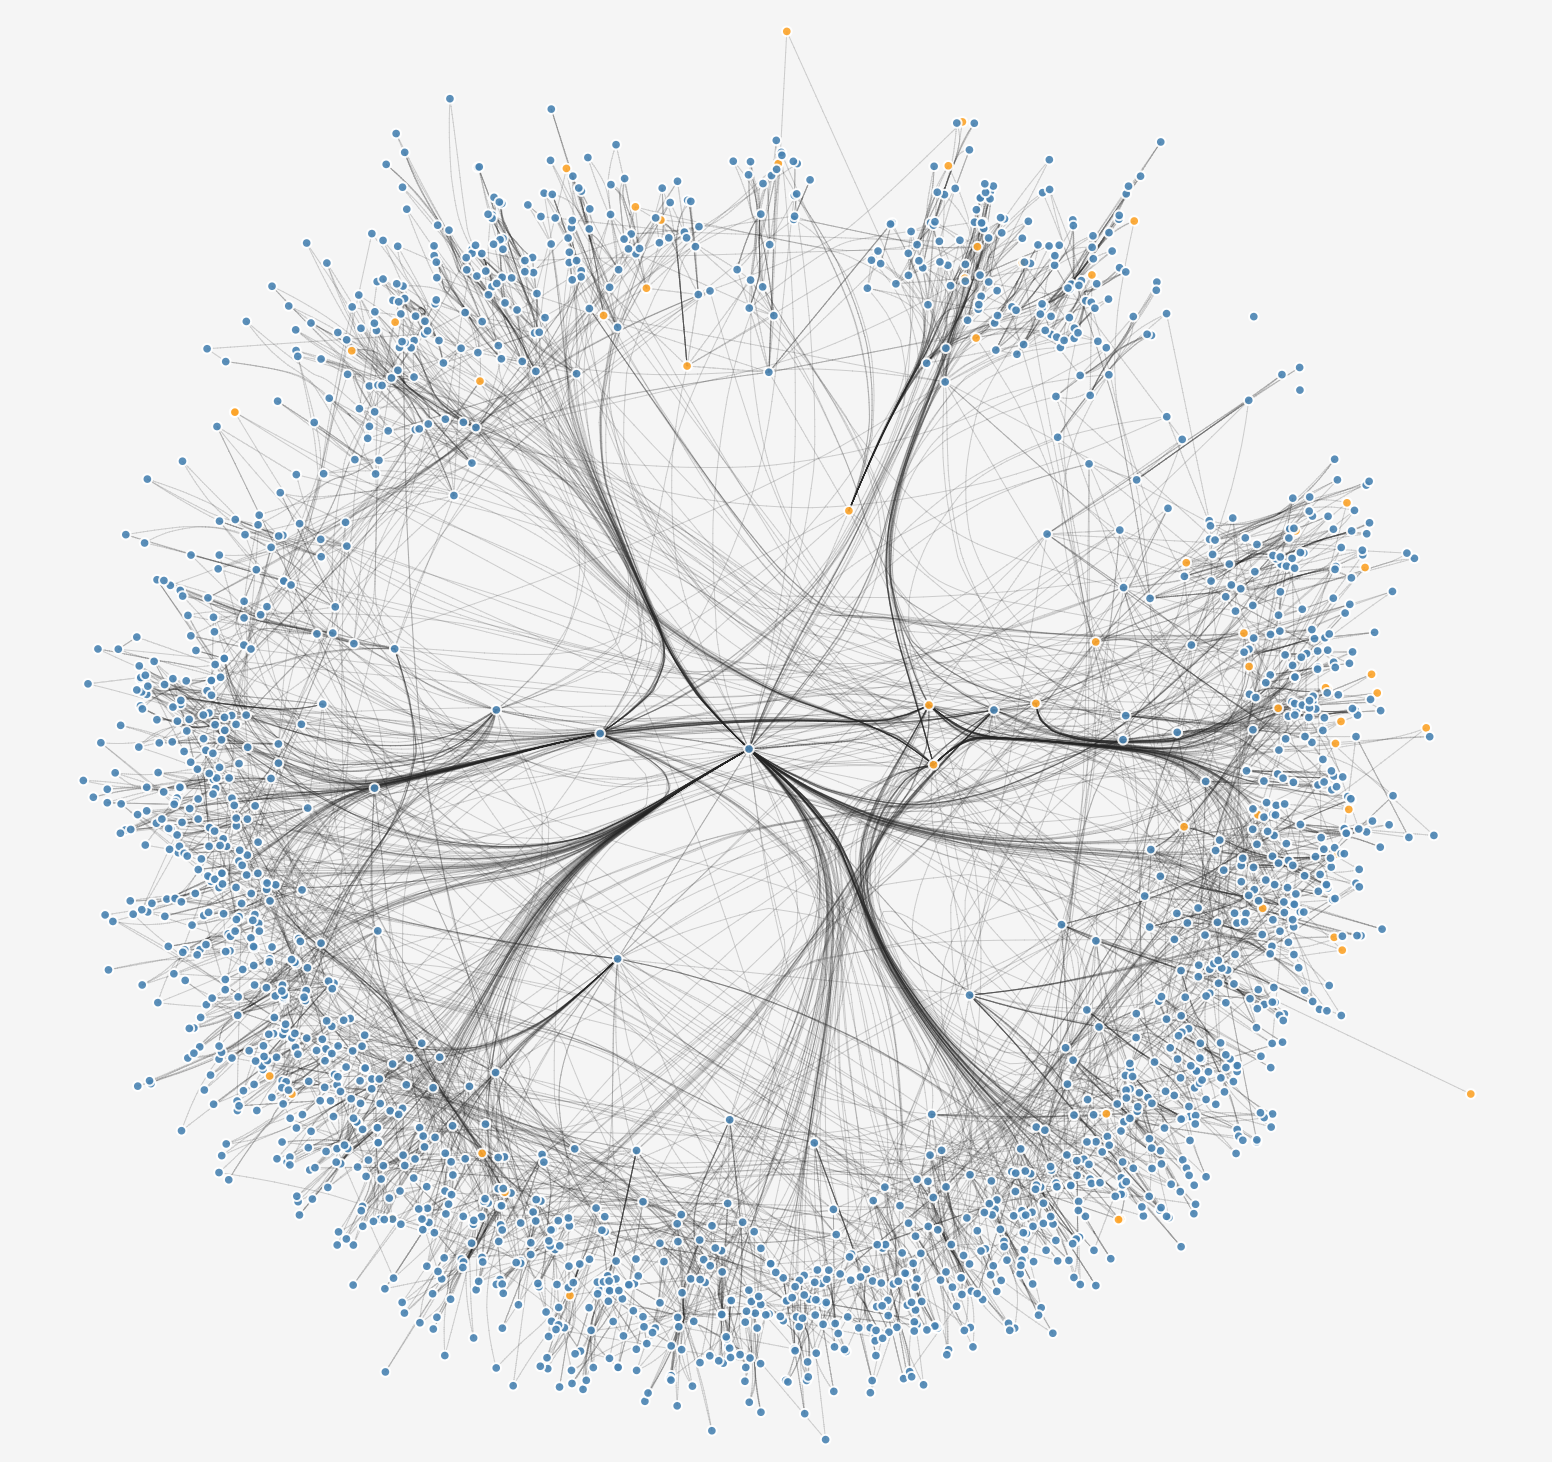
\includegraphics[width=\textwidth]{figures_c1/layout/merc4.png}
 \caption{$\theta = .65$}
 \end{subfigure}
        \caption{\textbf{How the compatibility threshold affects edge bundling.} In increasing the amount edges are attracted it is possible to improve the clarity of a graph. However there reaches a point where this distortion can worsen the result, confusing the reader, or creating a false positive. For this reason, I generaly use only a slight bundling value $> 0.7$.}
      \label{fig:edgebundling}
\end{figure}

\paragraph{Power, Routing and Confluence graphs.}

Confluent graphs use a graph drawing method in which edges are not drawn as individual distinguishable geometric objects, but rather as a crossing free system of arcs and junctions. \citep{confluient19}. Their design is similar to that of the edge bundling algorithm, except that rather than bundling edges spatially (a design which may introduce ambiguity), the bundling is done based on connectivity and can help reduce clutter by grouping multiple edges where the all target nodes are also connected to all the source nodes, \autoref{fig:confpic},\citep{confpic}. 

\begin{figure}[H]
     \centering
     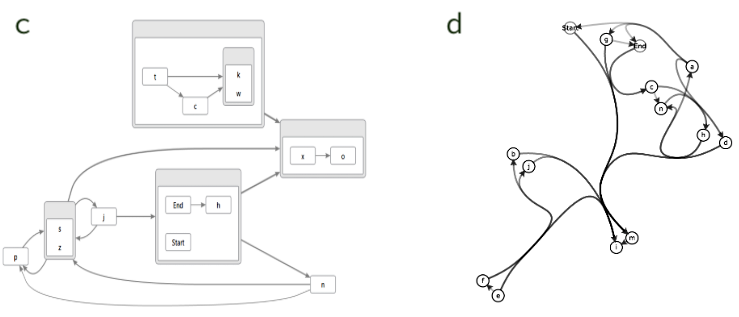
\includegraphics[width=.9\textwidth]{figures_c1/layout/confluent/example.png}
        \caption{\textbf{An example of confluent bundling. } From left to right -  A traditional network, Edge bundling, Power Graph and Confluent graph representations. Source: \citep{confpic}}
      \label{fig:confpic}
\end{figure}

Using butane as an example the construction of a confluent shall be covered. The first step in the process is to create
a power graph of our network. Power graphs are a representation of complex networks where sets of items identical source and target links are lumped or grouped within a single item. This is then converted into a routing graph, \autoref{fig:conf1}. To do this multiple edges which may be bundled have a `routing' node added to guide them. Next basis-splines, using the routing nodes as control points, are used to map the graph\footnote{These are similar to bezier curves but require a degree, $p$, $n+1$ control points, and a knot vector of $m+1$ points. Note: Knots are the things that make the curve continuous }, \autoref{fig:conf2}. Finally crossing links are removed, leaving the confluent graph, \autoref{fig:conf4}. 

Confluent drawings have been found to have many applications (e.g. the ego-centric author network and social interaction graph), they generally perform best in sparce networks with locally dense clusters of a tree like structure \citep{confluent17}. Although sparse, the cyclic nature of atmospheric chemistry does not allow for a sufficient reduction in complexity to make them a suitable improvement over traditional graphs. The use of very close fitting basis-splines in addition to a routing graph (confluent graph with crossing artifacts), may however help to simplify specific layouts or mechanism subsets with a certain amoung of tweaking. 

\begin{figure}[H]
     \centering
     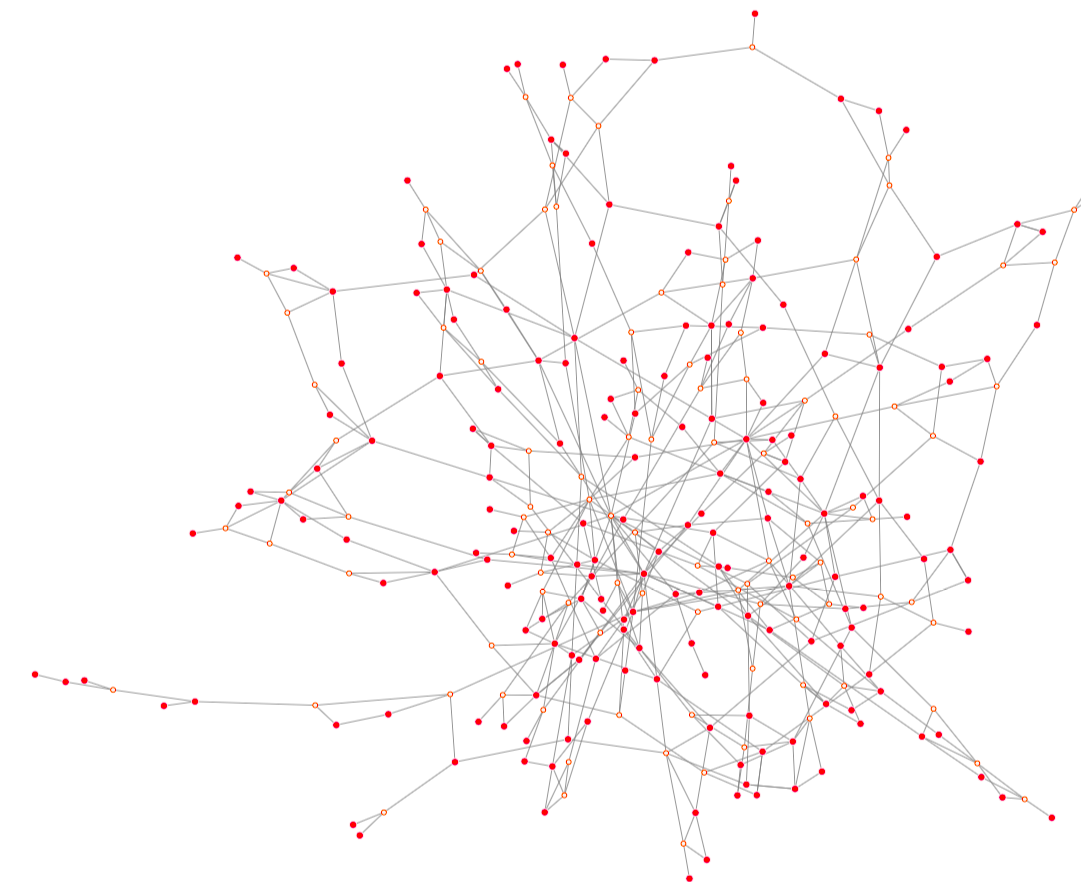
\includegraphics[width=.7\textwidth]{figures_c1/layout/confluent/1.png}
        \caption{\textbf{The routing graph of the butane mechanism.} Here paths which contain two or more bundles have an extra `routing' node introduced (orange stroke) }
      \label{fig:conf1}
\end{figure}

\begin{figure}[H]
     \centering
     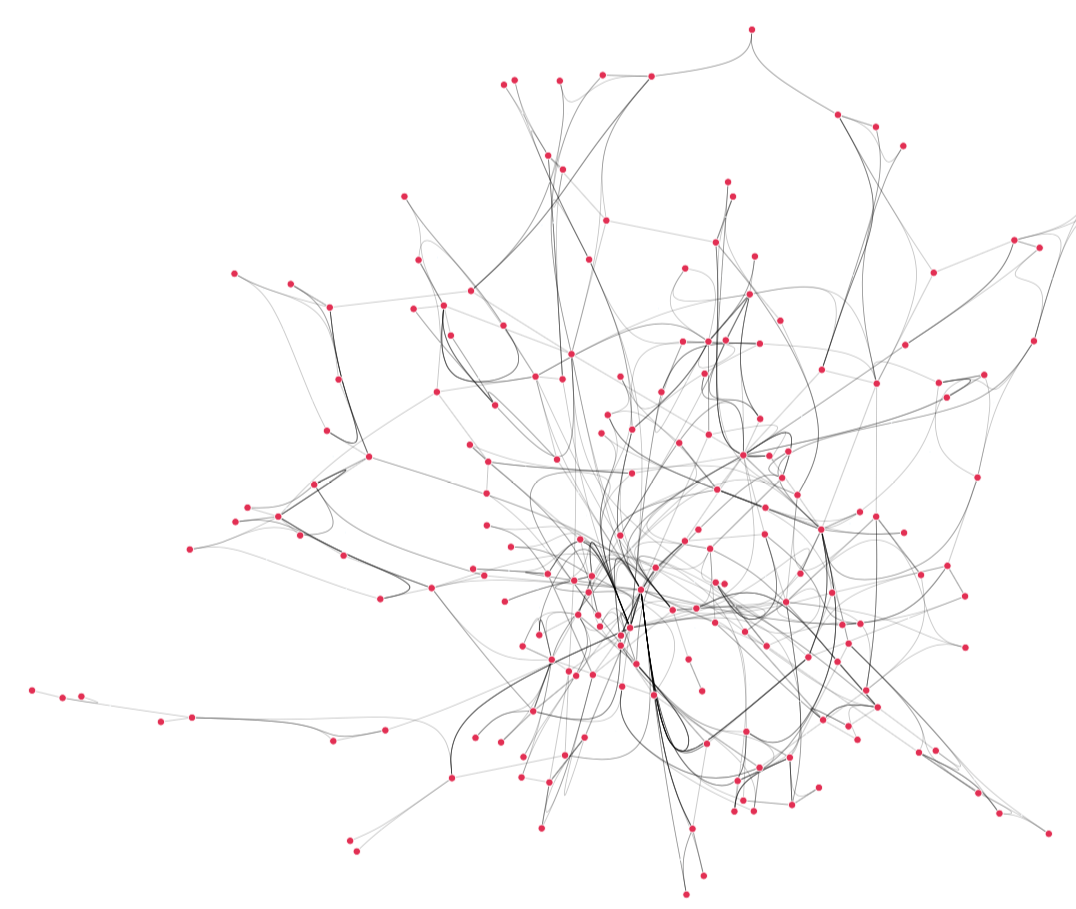
\includegraphics[width=.7\textwidth]{figures_c1/layout/confluent/2.png}
        \caption{\textbf{Confluent graph with crossing artifacts.} The routing graph with the addition of basis-splines using the orange routing nodes in \autoref{fig:conf1} as control points.}
      \label{fig:conf2}
\end{figure}

\begin{figure}[H]
     \centering
     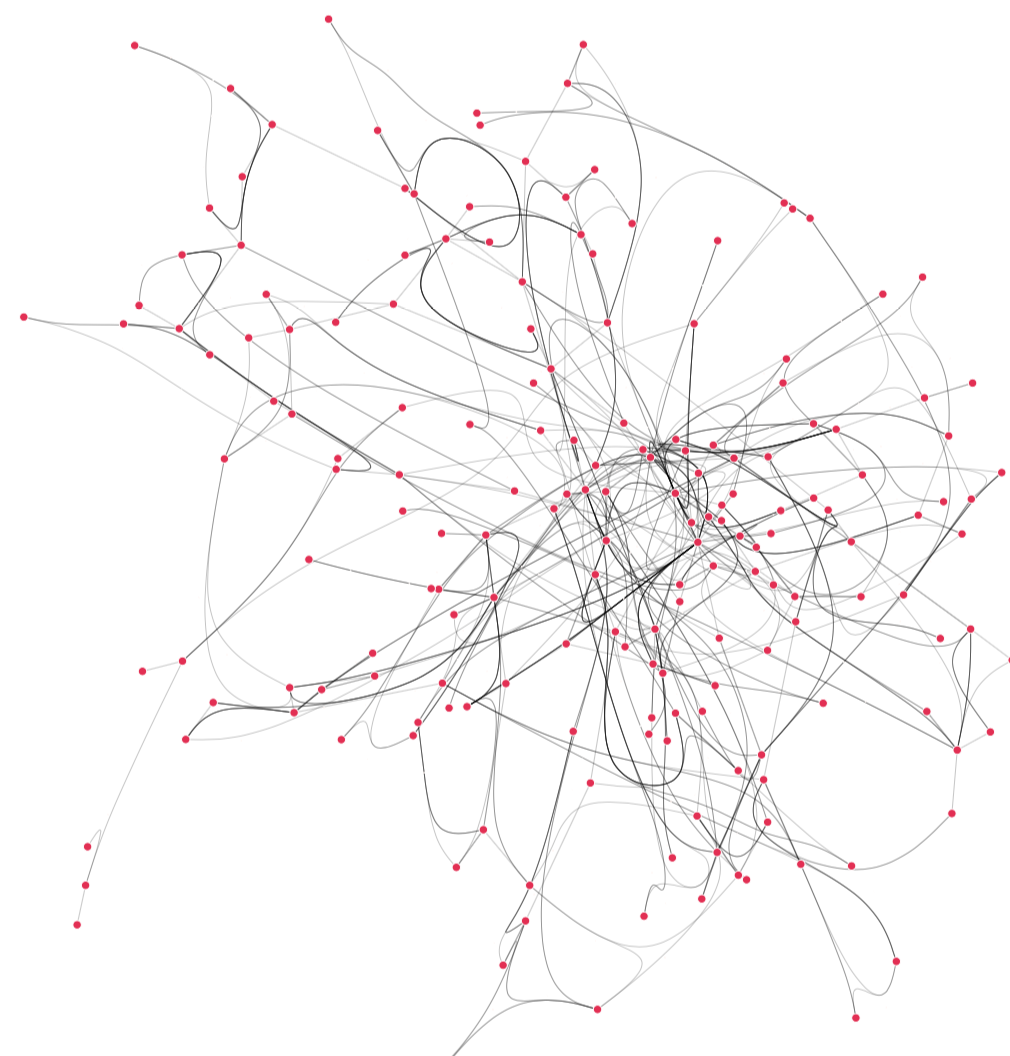
\includegraphics[width=.6\textwidth]{figures_c1/layout/confluent/4.png}
        \caption{\textbf{Confluent graphs without crossing artifacts.} The remaining confluent graph with crossing edges removed. }
      \label{fig:conf4}
\end{figure}



\paragraph{ Edge Angle / Continuity}
Visual representation utilises our conscious and unconscious pattern recognition and intuition abilities \citep{pattern}. To avoid apophenia (finding patterns where they do not exist), careful  consideration has to be placed in the design of a graph layout. 
Although edge corssing is ofthen though of as the most import aesthetic metric, finding a continuity between inward and outbound edges of a node was found to be if equal importance \citep{continuity}.

Reducing the angle between related edges increases readability and allows the behavioural process to infer information about a graph correctly. This process can be compared to predicting the direction of turbulent vs laminar flow. In addition to this edges should be spaced evenly around node, maximising the minimum-edge-angle between all edges of a node \citep{aestheticsgraphvis}. 



\subsection{Temporal Projection}
Story-telling has been an effective method to convey information, experience and cultural values for almost as long as people have been around. Many real-life physical processes occur over time and thus allow the use of a story-telling analogy. \citep{storytelling} provides a generic structure which begins with creating a general overview of the subject. Events are then animated in order of occurrence and defined as we go along. Finally any remaining conflicts and uncertainty is addressed, and these are rectified.  
Using this as a template for our graphs, we find that the content is usually given in the form of a title or figure description, the evolution as the visualisation, and finally the reflection and resolution through the use of user interaction (e.g., node hi-lighting, zoom or animation).

Since very few graph layouts support dynamic time-varying graphs \citep{tvg}, several methods of visualising temporal events have been developed. 
%Independent application to of these runs the risk of producing temporally incoherent visualisations. 
Although storylines can be useful for drawing the evolution of simple systems, these break down when dealing with large numbers of dependant variables. Force-directed layouts may be adapted, to suit these better, whereupon the initial positions of the previous node endpoints are used as the initial positions for consequential simulations. Three methods of representing these are shown in Figure \ref{temporal}.


\begin{figure}[H]
    \centering
     \begin{subfigure}[b]{.49\textwidth}
        \centering
    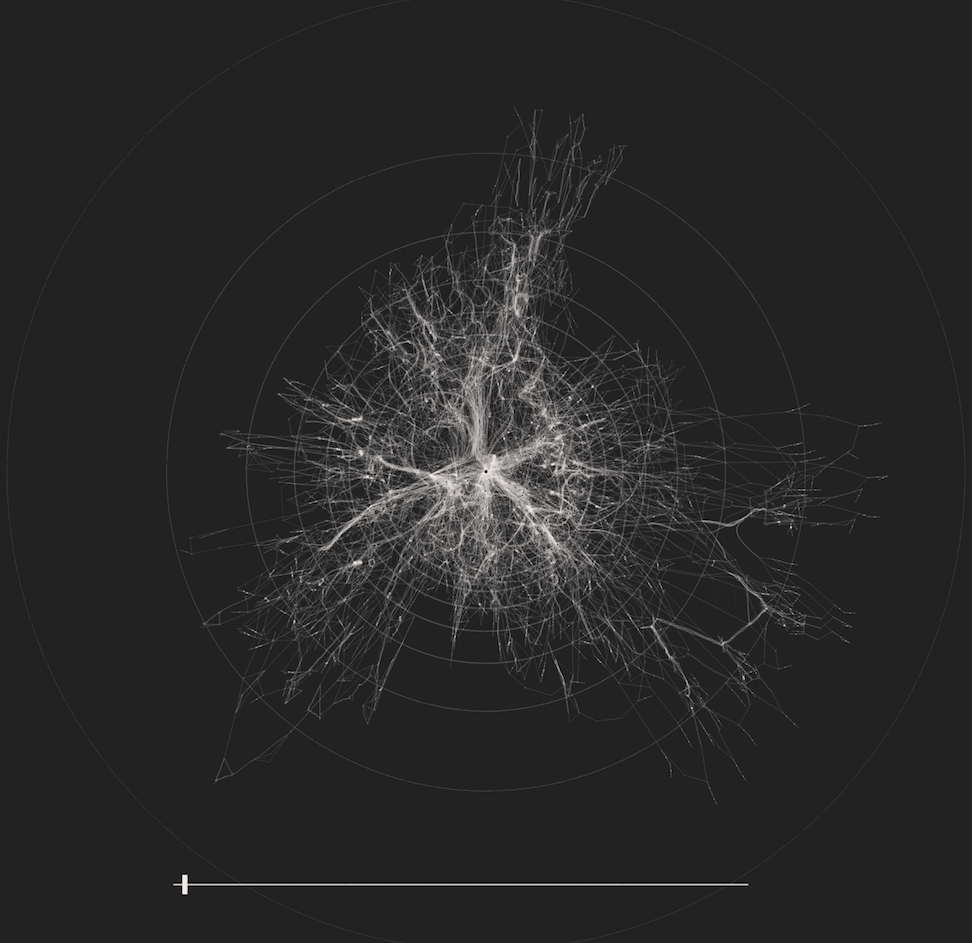
\includegraphics[width=\textwidth]{figures_c1/layout/confluent/0.png} 
    \caption{}
    \end{subfigure}
    \centering
     \begin{subfigure}[b]{.49\textwidth}
        \centering
    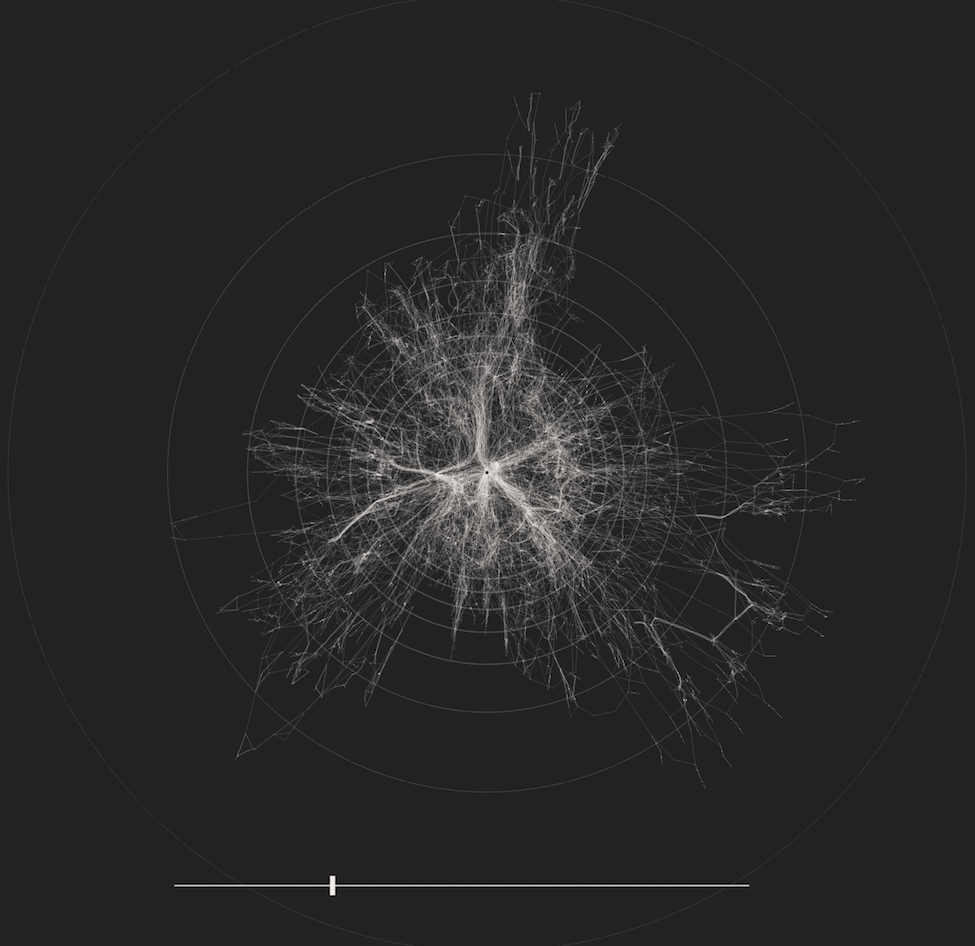
\includegraphics[width=\textwidth]{figures_c1/layout/confluent/25.png} \caption{}
    \end{subfigure}
    \centering
     \begin{subfigure}[b]{.49\textwidth}
        \centering
    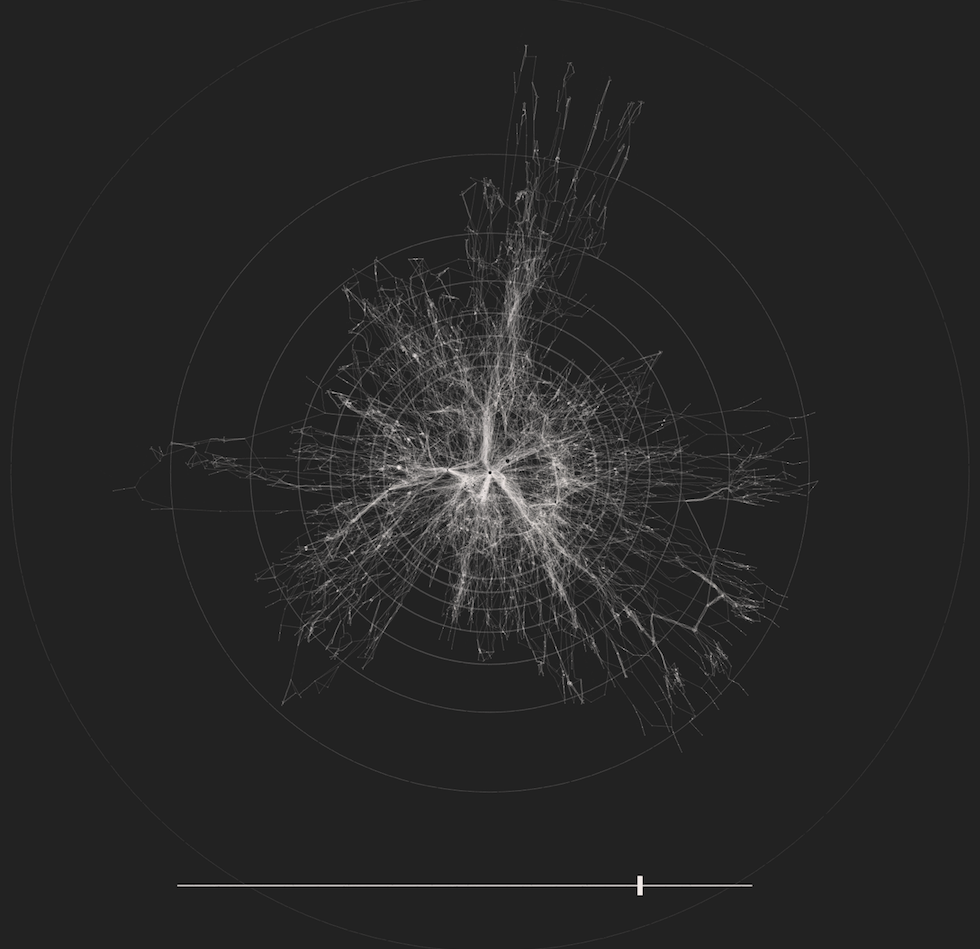
\includegraphics[width=\textwidth]{figures_c1/layout/confluent/75.png} 
    \caption{}
    \end{subfigure}
    \centering
     \begin{subfigure}[b]{.49\textwidth}
        \centering
    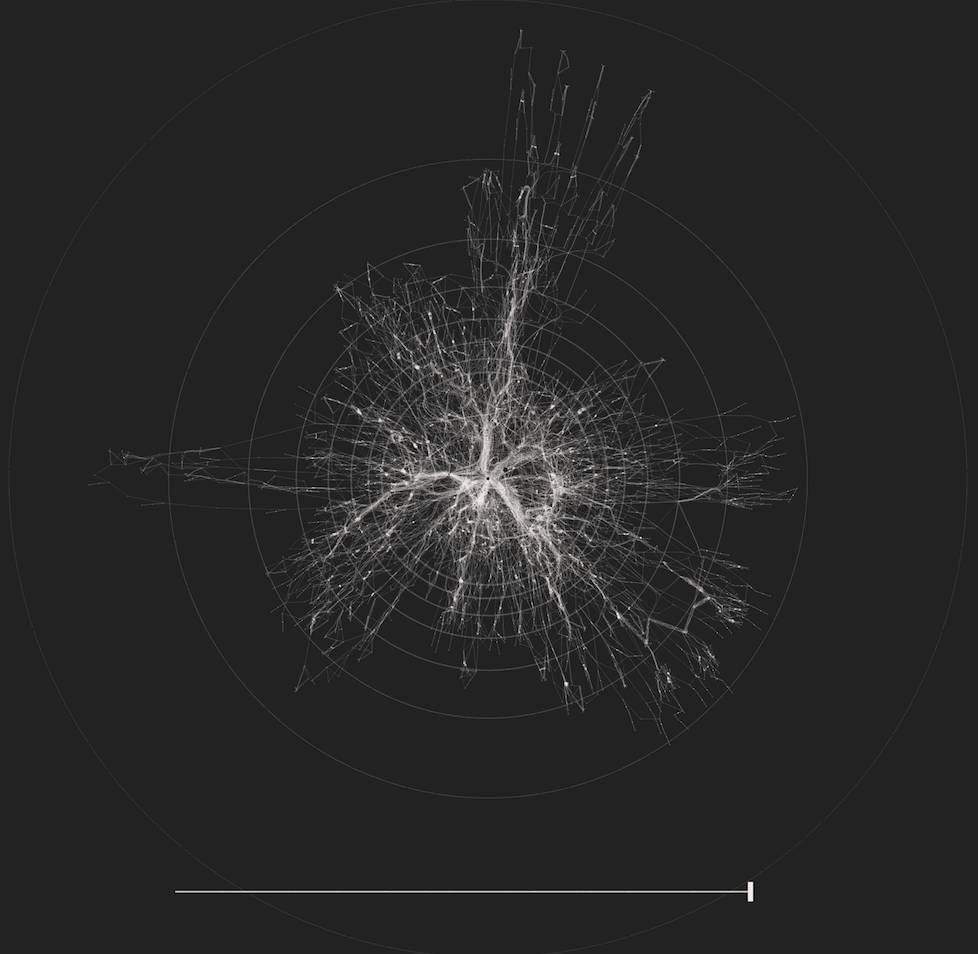
\includegraphics[width=\textwidth]{figures_c1/layout/confluent/100.png} 
    \caption{}
    \end{subfigure}
       \caption{\textbf{Film style representation of temporal changes in a network.} Showing the temporal changes from a model simulation of the beijing atmosphere. (a) shows a weighted graph at midnight. With the addition of daylight, the chemistry speeds up causing the force graph to contract, changing the overall network shape (the faster reactions have a stronger attractive force).}
     \label{fig:edgebundling}
\end{figure}


Finally, user-interaction such as hi-lighting key nodes/links, zoom and animation\footnote{\citep{ch8} notes that animation poses high demands on the users visual memory, and that snapshots are likely to miss underlying patterns.  For this reason an interactive techniques that can allow retrospective selection of timesteps allows for a good compromise between these.} may be used to clarify information at the reflection stage.

\subsection{Additional Dimensions}
Additional dimensions can be used to emphasise certain aspects of our graphs. For instance multiple layers may be used in a directional graph to separate the importance of the nodes \citep{IPSEPCOLA}. \autoref{3D} shows the first, second and third generation species of a mechanism containing isoprene in three dimensions. Such a visualisation may be explored interactively, with the aid of a computaional input device (a mouse, keyboard or device gyroscope), or with the aid of red-cyan 3D glasses (for non-interactive mediums such as print). 

 Different layers can be used to separate of primary VOCs, from species which result in their production (+1 layers) and loss (-1 layers).
 Temporal data, such as that in \autoref{temporal} can also be presented in this format. The only drawback is the high possibility of obfusciation which may result from many layers of overlapping information. 



\begin{figure}[H]
     \centering
     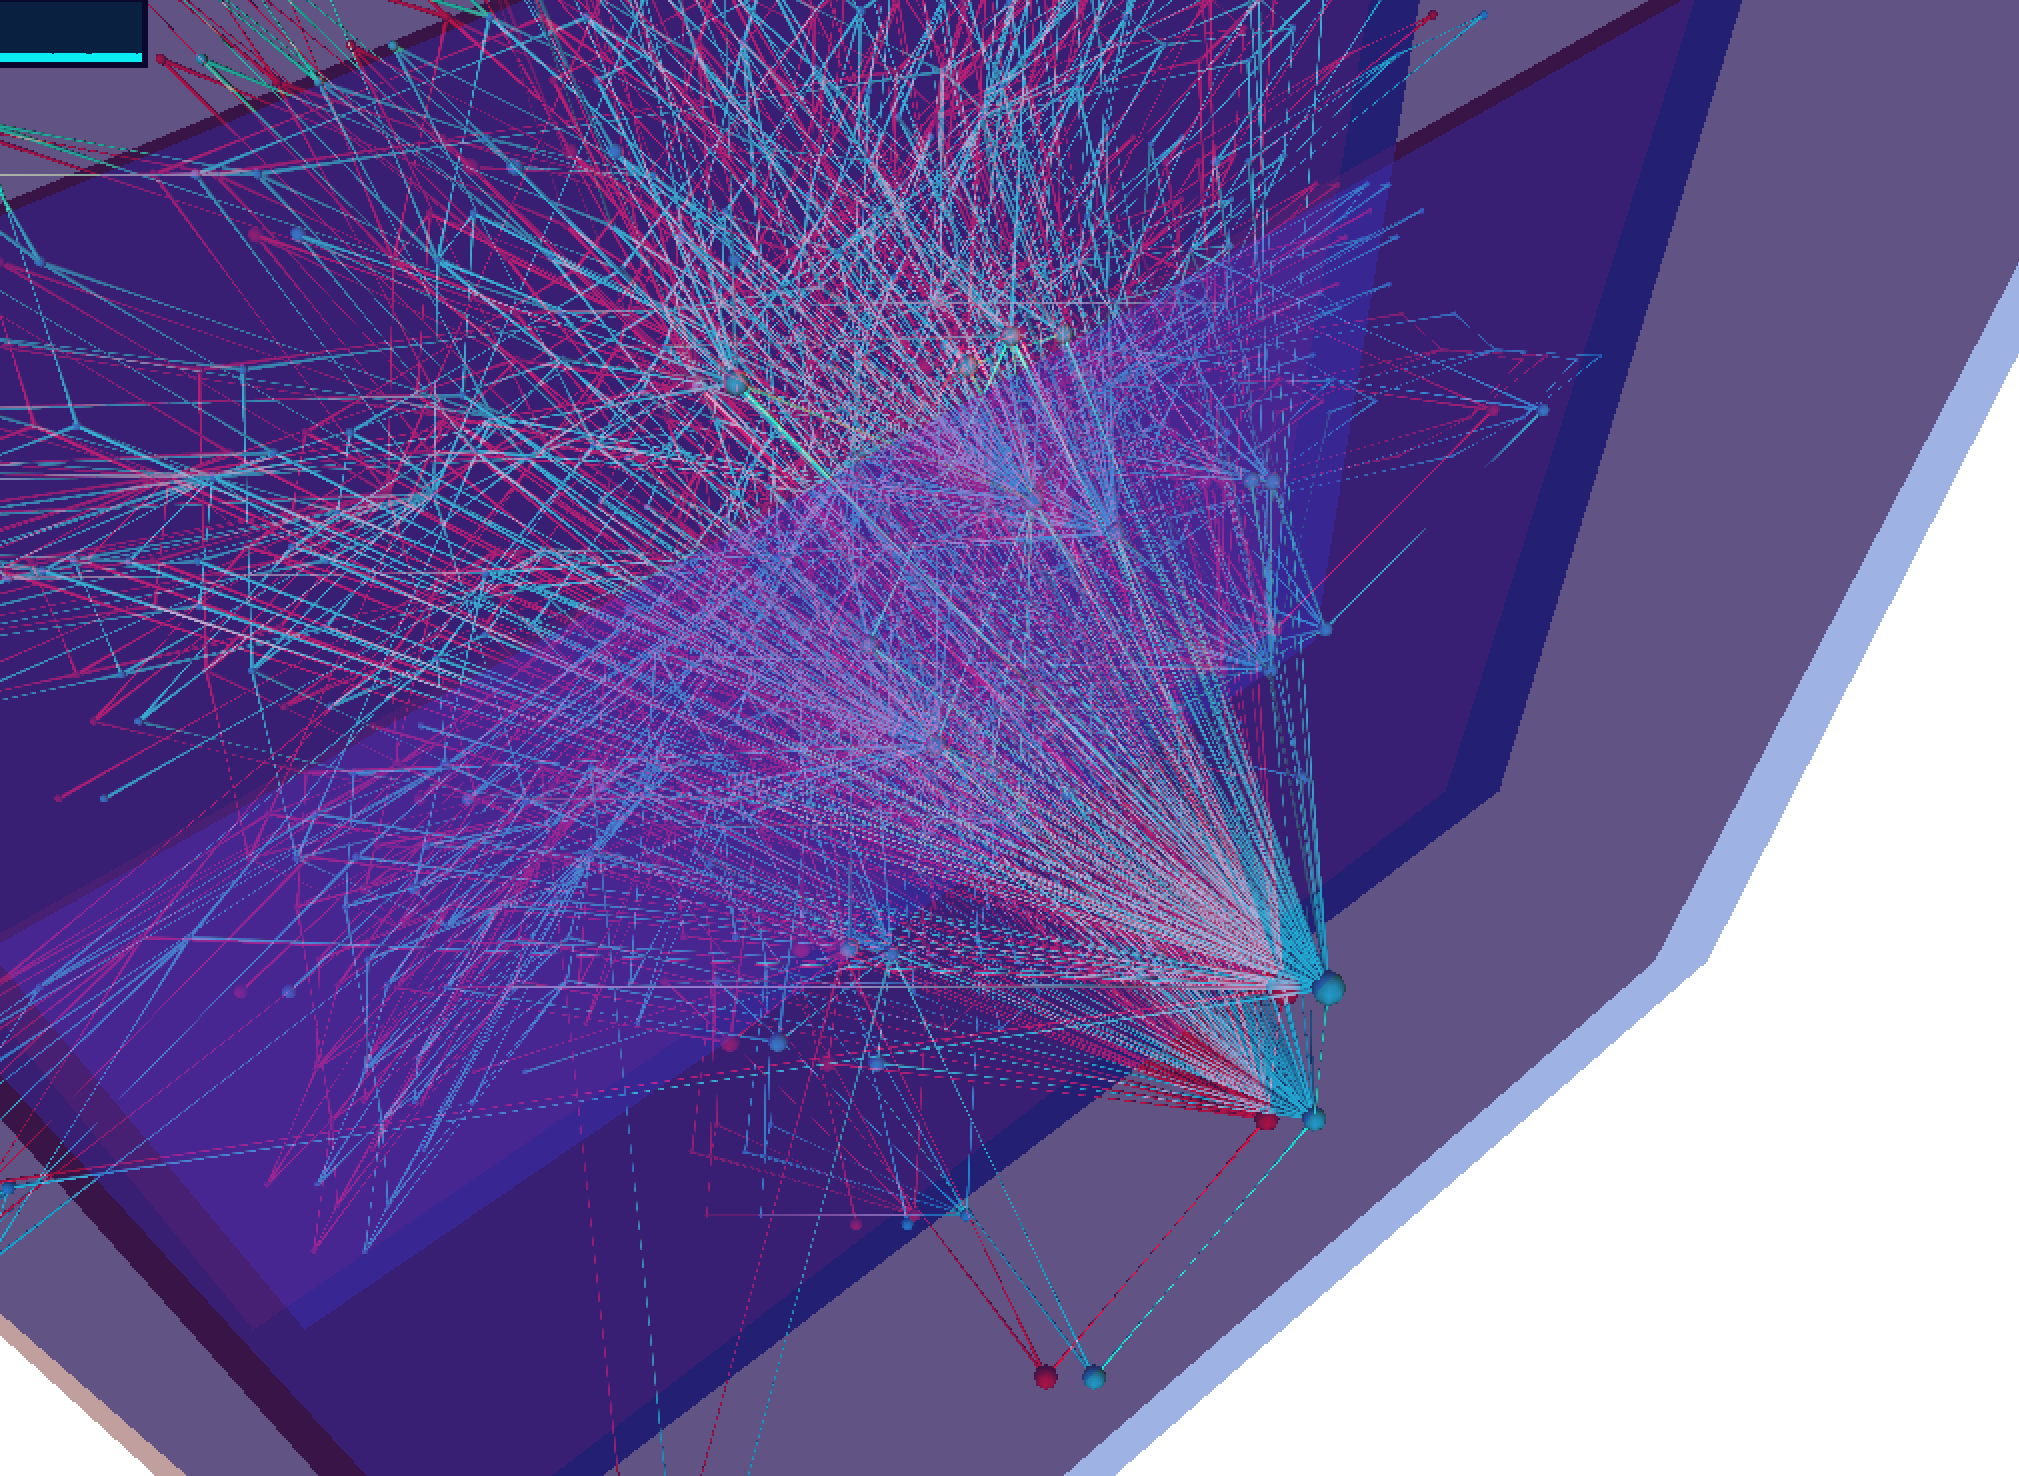
\includegraphics[width=.6\textwidth]{figures_c1/layout/3D.png}
        \caption{\textbf{A 3D representation of a graph to hilight certain features.} The first, second and third generation species of isoprene shown as an interactive 3D anaglyph. }
      \label{fig:3D}
\end{figure}




\section{A Chemistry Case Study}\label{sec:chemcase}
To conclude we apply many of the tools described above to a simple case study. We select a MCM subset containing methane as the only primary emitted species, and run it throught the Dynamically simple model of atmospheric chemical complexity (DSMACC) [ref] using the initial conditions of XYZ. We run this forwards to steady state and extract the flux between species on noon. The edge weight is the net flux (product of the species concentration * the rate of reaction for all reactions), normalised to a value between 1 and zero. 

This allows a simplified view of the different properties which affect the visualisation of the graph produced. 

\subsection{Syntatic Representation} 
Since we shall be using simulation data, we require a layout which deals with both direction and edge weights. In the spirit of zero and Protagoras\footnote{Famous for the phrase `man is the measure of all things' suggesting that we are constrained by our experiences}, we opt of the spring-like description presented by the Force Atlas 2 algorithm. This feature hi-lights fast reactions by bringing nodes together. Such a property has been observed to help users select the shortest path within a network \citep{eyetrack}. Here users picked the shortest path an average of 68\% for force directed graphs, compared to 40\% for hierarchical and 2\% for orthogonal layouts. Such properties can help us locate any trends in fast reactions which may control the chemistry within a system. 


\subsection{Semantic Representation}
Since the graph presented contains only a handful of species, our screen real-estate allows the listing of names for each node. Node sizes are scaled to represent the concentration of each species at that time point, and edges are coloured to represent the strength of each relationship between them. 


\begin{figure}[H]
     \centering
    \begin{subfigure}[b]{.4\textwidth}
         \centering
     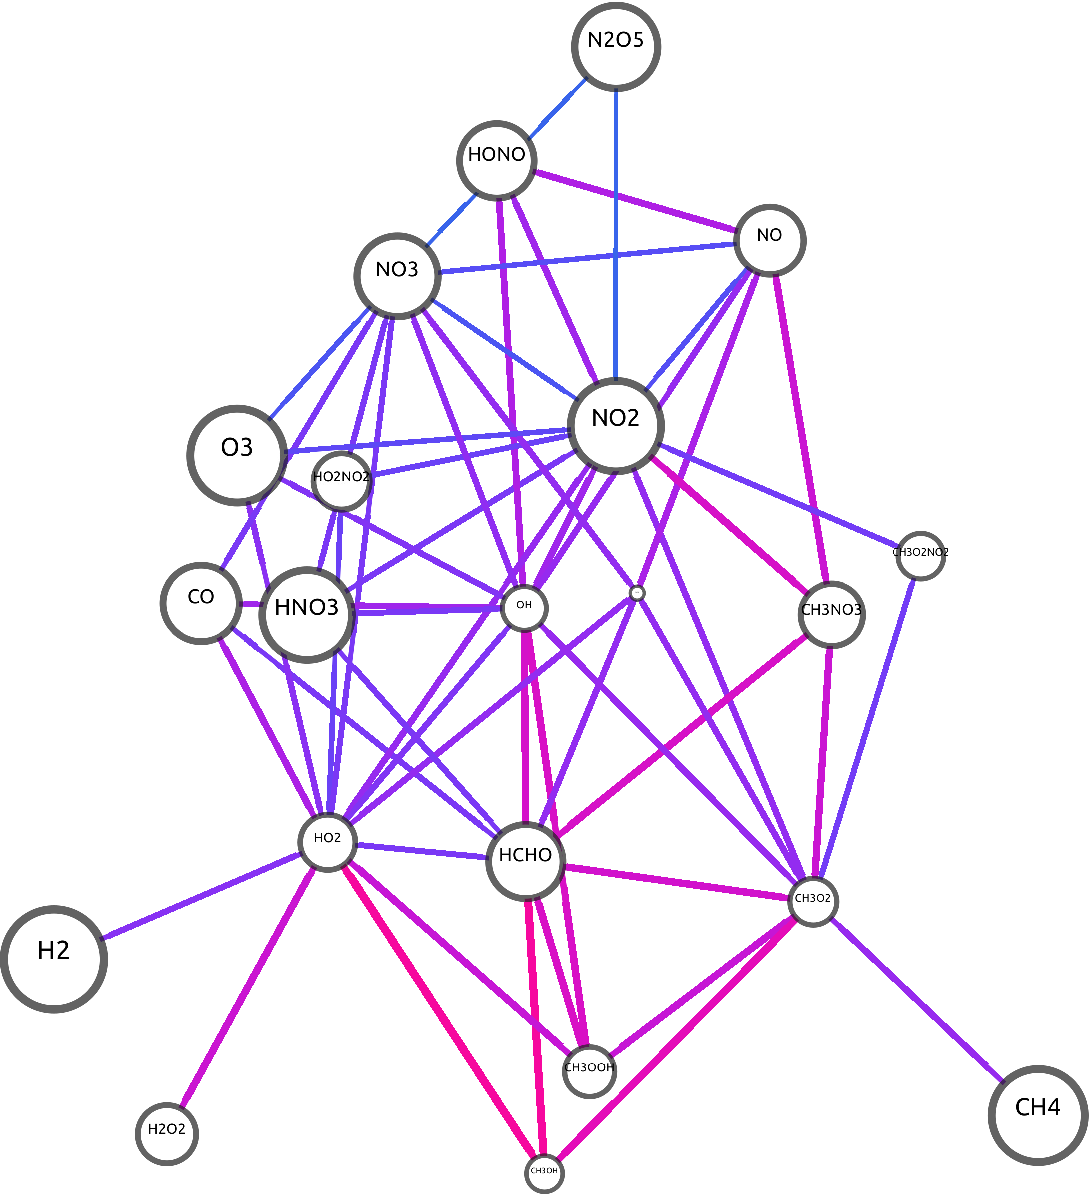
\includegraphics[width=\textwidth]{figures_c1/tap3/ch4_stretcheddefault-eps-converted-to.pdf}
     \caption{Connected unweighted}
     \end{subfigure}
     \begin{subfigure}[b]{.4\textwidth}
         \centering
     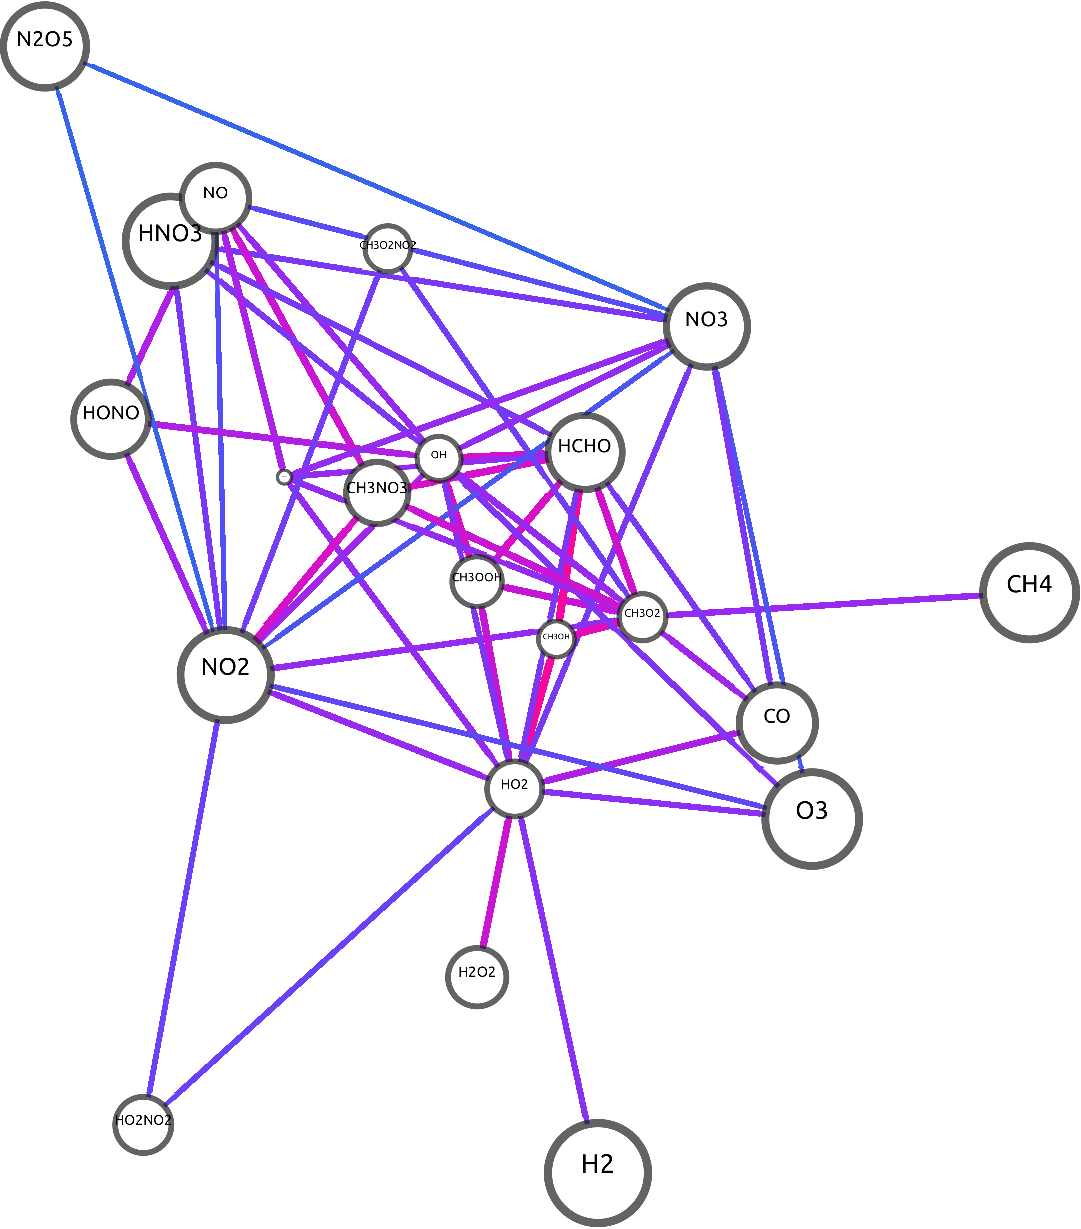
\includegraphics[width=\textwidth]{figures_c1/tap3/ch4_weighted_s1-eps-converted-to.pdf}
     \caption{Connected $\hat{\Gamma} = flux$}
     \end{subfigure}
        \caption{Basic steps within in the the graph production process}
      \label{fig:resmeth}
\end{figure}
% 
% \subsection{Local Vs Global Minimum }
% Since computers are deterministic, so are the calculations they perform\footnote{Within an absolute precision...}. In starting nodes from the same physical location and exerting the same force upon them, a force directed simulation will result in the nodes settling in the same locations. Since we use this `final' resting as the basis of our visual analysis, it is essential to find out if it represents the global minimum of the graph, or is merely a combination of the layout parameters and random seed. 
% 
% To do this we take a selection of 360 randomly initiated simulations, applying a monte carlo approach to simulation parameters and initial node placement. The force directed algorithm is then allowed to run with progressively decreasing energy until it reaches a stable equilibrium. Once this has been done we 
% 
% To ensure a global minimum has been met, a monte carlo approach with initial conditions is employed. Since a graph may hold both symmetrical and rotational symmetry, it is necessary to constrain the number of degrees of freedom it contains. The simplest way to do this would be to fix several nodes, and allow the force graph to evolve around this. Here we select the NO$_x$ species,$\{NO, NO_2,NO_3\}$, since their links form a triangle, and in doing so we can eliminate the rotational component of the algorithm. 
% 
% From here we allow the force directed algorithm to run until the nodes have settled, and record their positions. Once this has been done, all non-fixed nodes are given a random position and this whole process is repeated. 
% 
% 
% \subsubsection{Approximation Of Degrees Of Freedom} 
% Nodes with no connections can exist anywhere. Nodes which only have one connection, can only exist within a circle from the node they are bound to. If a node is connected  to two other nodes, it must therefore exist somewhere between them. This means that in general the more links a node has (its degree), the more constrained its location within the graph layout. 
% 
% 
% \begin{figure}[H]
%     \centering
%     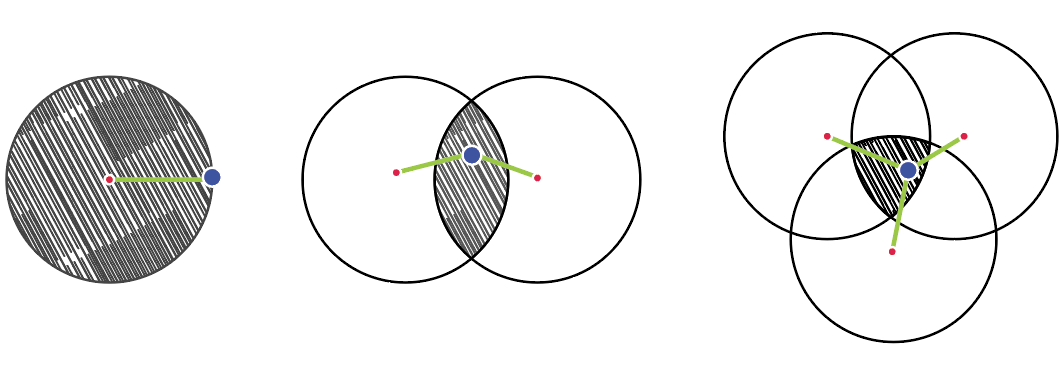
\includegraphics[width=.8\textwidth]{figures_c1/circles.png}
%     \caption{A demonstration on how the area / degrees of freedom (grey hashed area) of a node (blue) are limited by the number of neighbouring nodes it is anchored to (red) }
%     \label{fig:circle}
% \end{figure}
% 
% To test this we compare node degree with the dispersion between nodes in the above setup of the methane model. However since graphs are muli-link systems, the number of local minima for a specific node is not limited to direct links to its neighbours, their neighbours and so forth. To take this into account we device an \textit{approximate} metric - outlined below. 
% 
% \paragraph*{ A metric of establishing how mobile a node is within the force graph layout}
% As with all mathematical approximations we begin using a set of axioms. For this example we assume that: 
% \begin{itemize}
%     \item[1.] We have a set of fixed species, which we use to constrain the rotational symmetry of the graph with. In this case they are the NO$_x$ species.
%     \item[2.] A nodes `freedom' is mostly determined through the shortest path to all fixed species. 
%     \item[3.] We calculate the freedom by propagating the fraction of this constraint based on the number of links for each node, and propagating this forwards through the system
%     \item[4.] This metric is used as an effective indicator and not a complete calculation (where all possible paths should be used)
% \end{itemize}
% 
% \paragraph*{A worked example}
% To demonstrate this example we take an example shortest path (A-B-C-D) where A is fixed. Here B has 2 links, C has 3 and D has 4. The calculation of the freedom of D therefore equates to:
% \begin{center}
% \begin{multline} \\
%     A_{dof}  = 1\ (A\  fixed\  node)\\
%     B_{dof}  = A_{dof} /  2 = 1/2\\
%     C_{dof}  = B_{dof} /  3 = 1/6\\
%     D_{dof}  = C_{dof} /  4 = 1/24\\
% \end{multline}
% \end{center}
%  Finally inverse the values ($1-D_{dof}$) - such that the greater the output, the more freedom a node has in its final destination. 
% 
%  \paragraph*{Plotting correlation}
%  Using a setup of the $NO_{1-3}$ species (the red nodes: \autoref{fig:frmd_setup}) constrained in a triangle we run 1200 randomly initiated force directed graphs for the methane network and map the local minima obtained by each node at the end of each one.
% 
%   We then use this to calculate the deviation between each of these resting positions, their degree of freedom metric output and the node degree for each one. In looking only at the nodes connected to at-least one of the three fixed species, \autoref{fig:frmd_nox}, we see a pattern similar to that of \autoref{fig:circle}. Here the species \ce{CO,CH3O2NO2,HO2NO2} and \ce{CH3O2} all have a single link to a fixed species, and can disperse themselves evenly around these. Species with links to two fixed species, \ce{N2O5,HONO,O3,CH30} and \ce{CH3NO3}, are bulled between the two $NO_x$ species that they react with. Finally we have the hydroxide radical which reacts with all of the fixed species and is located at the centre of the triangle\footnote{As a note to clarify: although \ce{CH3O2} reacts with all three fixed groups, the construction methodology for this specific graph only take reactant-product pairs into account. As all of these are reactant-reactant reactions, they are not included within the graph.}.
% 
% 
% \begin{figure}[H]
%      \centering
%       \begin{subfigure}[b]{.38\textwidth}
%          \centering
%      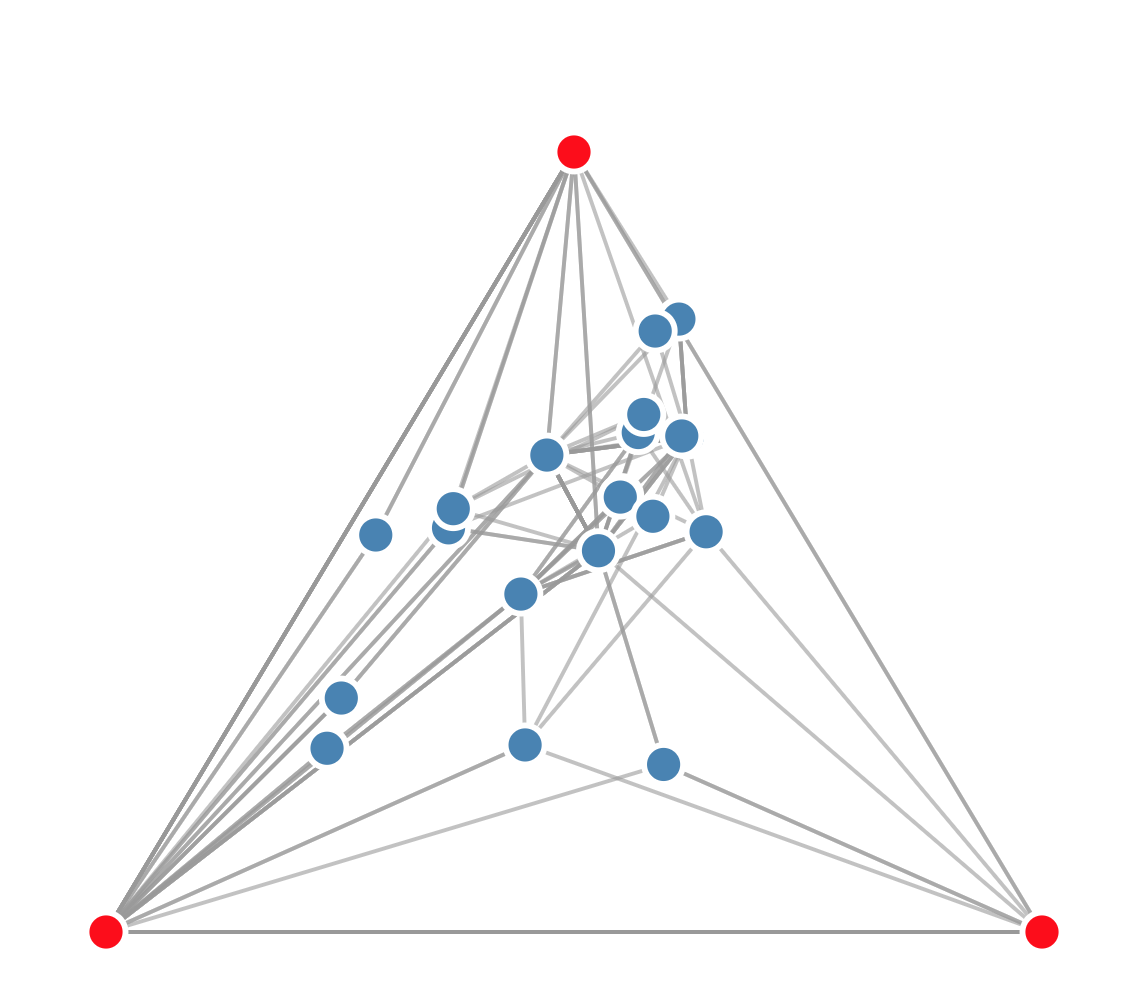
\includegraphics[width=\textwidth]{figures_c1/frmd.png}\vspace*{+8mm} 
%      \caption{The complete graph}
%      \label{fig:frmd_setup}
%      \end{subfigure}
%     \begin{subfigure}[b]{.45\textwidth}
%          \centering
%      \includegraphics[width=\textwidth]{figures_c1/frmd2.png}
%      \caption{Fixed node adjacent}
%      \label{fig:frmd_nox}
%      \end{subfigure}
%     %  \begin{subfigure}[b]{.32\textwidth}
%     %      \centering
%     %  \includegraphics[width=\textwidth]{figures_c1/frmd3.png}
%     %  \caption{Fixed node independant}
%     %  \label{fig:frmd_nonox}
%     %  \end{subfigure}
%         \caption{Showing the experimental force graph setup, with NO \ce{NO2} and \ce{NO3}  (red) fixed in position (\ref{fig:frmd_setup}). This     }
%       \label{fig:frmdstart}
% \end{figure}
% 
% 
%  To plot the correlation we use a Force Directed Representation of Multivariate Data (FRMD), written to show relationships between variables for data \citep{frmd}. This takes multivariate data and plots it in a inverse, fully connected graph\footnote{This is similar to the t-SNE dimensionality reduction technique [REF SECT]}. \autoref{fig:frmd_full} shows the a three dimensional comparison between a species deviation in resting position, degree and metric value.  Here nodes are connected to each category with a series of fixed `rods` or links. The length of each rod is adjusted such that it reflects the normalised value of its influence due to its origin category. This works by effectively `pushing` the node towards its category name. This allows us to partition the data into groups with similar properties, or extremes - for example \ce{CH3O2,HO2} and OH all have high degree values (>10 links) and low deviation in their local minimia locations. \ce{H2, CH3OH, CH3OOH} on the other hand have a wide range of possible local minima (deviation), which may be attributed to their low degree values. Formaldehyde on the other hand has both a great location deviation, as well as degree in general. These results suggest that for the higher metric values (small node size and near the bottom due to the 1-metric data set) the results are split between highly constrained species (due to a large number of links and a small deviation) and those which have many local minimia, and few links. 
% 
% 
% 
%  \begin{figure}[H]
%      \centering
%      \includegraphics[width=.8\textwidth]{figures_c1/fullold.png}\vspace*{+0mm} 
%      \caption{A plot showing the relationships between all three categories, and the links between them. Here we may identify groups of similar relationships, with the nodes close to a title having a high value in that feature, and ones near the middle containing a high value for all variables. \textbf{Values for the metric are 1-metric for this example.} }
%      \label{fig:frmd_full}
%      \end{figure}
% 
%      We can also reduce the number of dimensions of the FRMD visualisation from 3 to two. In taking only two features and encoding the third through either size or colour we can sometimes present a more unambiguous correlation between items. Within these visualisations we have imbalanced nodes on the horizontal, with higher values pushing the node towards its respective label. In cases where the relationship is approximately equal with both features the nodes exist on the vertical plane between each feature. Here low ranked equality lies close to the center line. Higher correlated matches are result in rods longer than the horizontal distance between both features. This causes a vertical displacement separating the nodes from the horizontal. 
% 
%      \autoref{fig:frmd_devdeg} shows the relationship between the location deviation and a nodes degree. Here, as with the 3 dimensional plot, we have a group of species which have a low degree coupled with a large location deviation, and a set of highly constrained species with >10 links. Similarly \ce{HCHO}, having a high number in both, is pushed away from the horizontal. As the metric value is encoded in the colour, we see that this has a stronger correlation with degree than deviation, which is expected since this plays a central role in the calculation of the freedom metric. 
% 
%     \begin{figure}[H]
%          \centering
%      \includegraphics[width=\textwidth]{figures_c1/devdeg.png}
%      \caption{Comparing deviations in node location with the number of links that species has within the reaction graph (degree) using a 2D version of the FRMD software. A node's importance with respect to the metric is embedded within the nodes colour and size.}
%      \label{fig:frmd_devdeg}
%      \end{figure}
% 
% 
% 
% Having shown how node degree fares against the actual deviation of each node, it is time to compare this against our metric. In \autoref{fig:frmd_devmet} we see a much narrower band of nodes along the horizontal. This suggests a better correlation between the two values - the ranking within each category are of a similar magnitude. 
% 
% 
%      \begin{figure}[H]
%          \centering
%      \includegraphics[width=\textwidth]{figures_c1/frmd_devmet.png}
%      \caption{Exploring how node deviation varies with the freedom metric above. Node colour and size represent the degree of each node, and are represented using the FRMD model. }
%      \label{fig:frmd_devmet}
%      \end{figure}
% 
% 
% 
% 
% 
%  \newpage
% 
% %trim={<left> <lower> <right> <upper>}


\section{A Model Of Beijing}
Using a spun up model initiated from the campaign results XX Beijing (Where did I get these?) we compare the distribution of links within a model. In f[FIG XX] we see the graph shape change due to the presence of photons. 


To perform a sensitivity study on the initial positions of nodes within the force atlas algorithm, a graph consisting of links and weightings is constructed using a box model simulation of the Beijing summer environment at mid-day and feed it the gephi software \citep{gephi} - an open source software designed for the exploration of networks. We then scrip the java code to perform the functions in \autoref{fig:flowrepeat}. As part of this, nodes are initiated with a random position, the force atlas 2 layout is then run and then the graph is rotated and translated such that it is centred around carbon monoxide and has a 45 degree angle between this and formaldehyde. This step constrains the general orientation of the graph, allowing us to analyse the generated graphs for global and local minima. The final step is to save a copy of the generated graph layout and repeat to generate a data set, a subset of which is shown in  \autoref{fig:all}

    \begin{figure}[H]
         \centering
     \includegraphics[width=\textwidth]{figures_c1/flowrepeat.png}
     \caption{ A flow chart of the process performed by the custom gephi script used to generate the data set}
     \label{fig:flowrepeat}
     \end{figure}
 
    \begin{figure}[H]
         \centering
     \includegraphics[width=\textwidth]{figures_c1/beijingtest/10_900.png}
     \caption{A sample of the 900 graphs generated using the force atlas 2 algorithm for the simulation output representative of the summer beijing chemistry at noon.  }
     \label{fig:all}
     \end{figure}
 

\subsubsection{Trends In The Chemistry}
Due to the construction protocols of the master chemical mechanism, \autoref{fig:protocol}, primary emitted compounds are oxidised to produce a cascade of species, ultimately ending at carbon dioxide\footnote{The MCM conserves the number of carbons, allowing \ce{CO2} to be introduced.} and water. As this process is central to the construction of the mechanism, it follows that they may be used to explain any features uncovered using the network layout. 

\paragraph{Network shape}\label{sec:netshape}
Using \autoref{fig:all} the pattern recognition capabilities of the human mind identify a certain shape associated with many of the networks. Upon closer inspection it may be hypothesized that the chemistry is split into three main branches. \autoref{fig:colour} categorises all the primary emitted species, and then uses voronoi tessellation\footnote{see chapter xxx for an example of this} to colour neighbouring nodes and their links by the classification of the closest primary emitted species. Using this it is possible to separate the MCM network into an aromatic branch, a terpene branch, an alkane and straight chain alkene branches. Such branches not only help us identify changes of chemistry due to biogenic or anthropogenic sources, but also emphasise the path taken to carbon dioxide and water. Since the MCM does not contain \ce{CO2} we see all the different groups converge on Carbon Monoxide (white, centre). Using this format, we may now compare the orientation of the many automatically generated layouts.  
 
    \begin{figure}[H]
         \centering
    %  \includegraphics[width=\textwidth,trim={0 4cm 0 4cm}]{figures_c1/beijingtest/graphgroups.pdf}
    \includegraphics[width=\textwidth,trim={0 4cm 0 4cm},angle=-90]{figures_c1/beijingtest/graphgroups.pdf}
     \caption{Hi-lighting the groups of species, and their products within the MCM network graph. These are {\color{DarkGoldenrod} Aromatics (gold)} , {\color{DarkTurquoise} terpenes (turquoise) } and {\color{OrangeRed} Alkane}/{\color{RoyalBlue} Alkene  } carbon chains (red/blue)}
     \label{fig:colour}
     \end{figure}

\paragraph{Pattern Matching using t-SNE}
t-Distributed Stochastic Neighbor Embedding (t-SNE) is a dimensionality reduction technique used in automatic categorisation of images or photographs \citep{truthandbeauty,sketchy}. This is the same process as referenced in EARLIERREF and described in detail within Chapter... 

To compare the generated networks, we flatten the pixel matrix for each centered image in the dataset, and assign the output list to each filename. The resultant dataframe is then fed into the t-SNE algorithm in the Scikit Learn package \citep{scikit-learn}. This reduces the logical list of pixels for each image into a two dimensional representation of their similarity. We plot each file, for its $(x,y)$ coordinate, and isolate clusters of similarity using density contours in 

    \begin{figure}[H]
         \centering
    \includegraphics[width=.6\textwidth]{figures_c1/beijingtest/density.png}
     \caption{\textbf{A normalised scatter plot of 2D space produced by the t-SNE algorithm.} Each triangle represents a different file, and the colours/density contours show the regions in which we find similar images/graphs. }
     \label{fig:densty}
     \end{figure}

Using interactivity and/or vector cluster detection techniques it is possible examine which files contribute to an area of high density. \autoref{fig:densitypic} shows a sample of four graphs from each corresponding cluster. Although individual node locations may vary, patterns on the macro scale start to emerge, with similar groups exhibiting symmetrical symmetry, e.g. groups 1/2 and 3/4. This suggests a constraint in the overall degree of freedom can be attributed solely to the network structure, and consequently the chemistry which forms this. The non-random nature of the produced graph layouts mean that it would be possible to juxtapose a variety or mechanisms using the force atlas 2 layout.

\begin{figure}[H]
     \centering
     \begin{subfigure}[b]{.2\textwidth}
         \centering
     \includegraphics[width=\textwidth]{figures_c1/beijingtest/1.png}
     \caption{Group 1}
     \end{subfigure}
     \begin{subfigure}[b]{.2\textwidth}
         \centering
     \includegraphics[width=\textwidth]{figures_c1/beijingtest/2.png}
     \caption{Group 2}
     \end{subfigure}
     \begin{subfigure}[b]{.2\textwidth}
         \centering
     \includegraphics[width=\textwidth]{figures_c1/beijingtest/3.png}
     \caption{Group 3}
     \end{subfigure}
     \begin{subfigure}[b]{.2\textwidth}
         \centering
     \includegraphics[width=\textwidth]{figures_c1/beijingtest/4.png}
     \caption{Group 4}
     \end{subfigure}
        \caption{\textbf{A selection of graphs corresponding to the labeled clusters in \autoref{fig:densty}}. These reveal that symmetric similarity between like-positioned points within the t-SNE output.  }
      \label{fig:densitypic}
\end{figure}

% \subsubsection{Location Analysis And Lifetime}
% In the previous subsection it was shown that the force atlas algorithm can be used to hi-light trends within the chemistry of a mechanism. Since the concentration change of a species depends on a range of factors which change throughout the length of a simulation, it follows that the force-directed graph generated for different timesteps may vary. Using the same setup as above we compare the network at noon (REF) and midnight (ref). 
% 
% \paragraph*{Diurnal Changes}\label{sec:diurnal}
% 
% 
% 
% 
% \paragraph*{Species Lifetime}
% 



\section{Summary}
Representing data in a visual format can be used to (utilise) the pattern recognition side of the human brain and alleviate the cognitive strain produced by numerical data. This is a technique used by the Samaritans (YEAR) with the use of cuneiform, and proved useful throughout. 

In designing a visualisation it is important to use storytelling and select metaphors familiar to the reader. This should be paired with the correct encoding, as to reduce the time spent trying to comprehend a figure, and increase the knowledge transfer. [ref chapter 1]

When considering relationships, one such analogy lies in the ball and stick analogy. Much like holding hands, this symbolises a similarity between connected items and is the basis of a mathematical graph, or network. Such representations can be applied to the chemical complexity shown in species within the atmosphere. 

In representing the chemistry within a mechanism as a graph we may visualise it with the use of a force-directed layout. These are in essence a simple physical simulation, whereupon each graph node is repelled (like-charge), and connected nodes joined by a spring-like attractive force. It is found that the force atlas 2 algorithm not only produces the best visual aesthetic, but also conceptual understanding. Using this it is possible to see patterns such as the the partitioning of each network into aromatic, terpene and straight chain chemistry. 

Although graph layouts have a range of local minima, the overall network structure of the MCM is constrained by its construction protocol (due to the allowed chemical reactions), and thus can be used to produce comparable graphs. This method of visualisation, in combination with interactive querying techniques, can aid in the comparison and understanding of large/complex chemistry simulations. This can be particularly useful in the explanation of specific interactions within a mechanism, or the exploration of temporal changes within a simulation. 

In the next chapter, I shall extend the graph metaphor for atmospheric chemistry systems beyond that of just visualisation. 
